\documentclass[11pt,a4paper,dvipsnames]{article}
\usepackage[margin=2.5cm]{geometry}
\usepackage{iohk}
\usepackage{microtype}
\usepackage{mathpazo} % nice fonts
\usepackage{amsmath}
\usepackage{amssymb}
\usepackage{amsthm}
\usepackage{latexsym}
\usepackage{mathtools}
\usepackage{stmaryrd}
\usepackage{extarrows}
\usepackage{slashed}
\usepackage[colon]{natbib}
\usepackage[unicode=true,pdftex,pdfa,colorlinks=true]{hyperref}
\usepackage{xcolor}
\usepackage[capitalise,noabbrev,nameinlink]{cleveref}
\usepackage{float}
\floatstyle{boxed}
\restylefloat{figure}
\usepackage{tikz}
\usepackage{booktabs}
\usepackage{enumerate}


%%
%% Package `semantic` can be used for writing inference rules.
%%
\usepackage{semantic}
%% Setup for the semantic package
\setpremisesspace{20pt}

%%
%% Types
%%
\newcommand{\Nothing}{\ensuremath{\Diamond}}
\newcommand{\N}{\ensuremath{\mathbb{N}}}
\newcommand{\Bool}{\type{Bool}}
\newcommand{\Npos}{\ensuremath{\mathbb{N}^{+}}}
\newcommand{\Z}{\ensuremath{\mathbb{Z}}}
\newcommand{\R}{\ensuremath{\mathbb{R}}}
\newcommand{\Rnn}{\ensuremath{\mathbb{R}^{\geq 0}}}
\newcommand{\Tx}{\type{Tx}}
\newcommand{\TxBody}{\type{TxBody}}
\newcommand{\TxWitness}{\type{TxWitness}}
\newcommand{\Ix}{\type{Ix}}
\newcommand{\TxId}{\type{TxId}}
\newcommand{\Addr}{\type{Addr}}
\newcommand{\UTxO}{\type{UTxO}}
\newcommand{\Wdrl}{\type{Wdrl}}
\newcommand{\Coin}{\type{Coin}}
\newcommand{\PParams}{\type{PParams}}
\newcommand{\Slot}{\type{Slot}}
\newcommand{\SlotsPrior}{\ensuremath{\mathsf{SlotsPrior}}}
\newcommand{\SlotsPerEpoch}{\mathsf{SlotsPerEpoch}}
\newcommand{\SlotsPerKESPeriod}{\mathsf{SlotsPerKESPeriod}}
\newcommand{\Duration}{\type{Duration}}
\newcommand{\StakePools}{\type{StakePools}}
\newcommand{\StakeKeys}{\type{StakeKeys}}
\newcommand{\Seed}{\type{Seed}}
\newcommand{\seedOp}{\star}
\newcommand{\Ppm}{\type{Ppm}}
\newcommand{\Value}{\type{Value}}
\newcommand{\ProtVer}{\ensuremath{\type{ProtVer}}}
\newcommand{\ApName}{\ensuremath{\type{ApName}}}
\newcommand{\ApVer}{\ensuremath{\type{ApVer}}}
\newcommand{\SystemTag}{\ensuremath{\type{SystemTag}}}
\newcommand{\UpdateData}{\ensuremath{\type{UpdateData}}}
\newcommand{\Metadata}{\ensuremath{\type{Mdt}}}
\newcommand{\PPUpdate}{\type{PPUpdate}}
\newcommand{\Applications}{\type{Applications}}
\newcommand{\AVUpdate}{\type{AVUpdate}}
\newcommand{\Update}{\type{Update}}

\newcommand{\DCert}{\type{DCert}}
\newcommand{\DCertRegKey}{\type{DCert_{regkey}}}
\newcommand{\DCertDeRegKey}{\type{DCert_{deregkey}}}
\newcommand{\DCertDeleg}{\type{DCert_{delegate}}}
\newcommand{\DCertRegPool}{\type{DCert_{regpool}}}
\newcommand{\DCertRetirePool}{\type{DCert_{retirepool}}}
\newcommand{\DCertGen}{\type{DCert_{genesis}}}
\newcommand{\PoolParam}{\type{PoolParam}}
\newcommand{\UTxOState}{\ensuremath{\type{UTxOState}}}
\newcommand{\ledgerState}{\ensuremath{\type{ledgerState}}}

\newcommand{\AddrRWD}{\type{Addr_{rwd}}}
\newcommand{\AddrB}{\type{Addr_{base}}}
\newcommand{\AddrP}{\type{Addr_{ptr}}}
\newcommand{\AddrE}{\type{Addr_{enterprise}}}
\newcommand{\AddrBS}{\type{Addr_{bootstrap}}}
\newcommand{\Ptr}{\type{Ptr}}
\newcommand{\DState}{\type{DState}}
\newcommand{\DWEnv}{\type{DWEnv}}
\newcommand{\DPSEnv}{\type{DPSEnv}}
\newcommand{\DPEnv}{\type{DPEnv}}
\newcommand{\DEnv}{\type{DEnv}}
\newcommand{\PEnv}{\type{PEnv}}
\newcommand{\DPState}{\type{DPState}}
\newcommand{\PState}{\type{PState}}
\newcommand{\DCertBody}{\type{DCertBody}}
\newcommand{\TData}{\type{TData}}
\newcommand{\DPoolReap}{\ensuremath{\type{poolreap}}}
\newcommand{\UPIState}{\type{UPIState}}
\newcommand{\UpdatePayload}{\type{UpdatePayload}}

% multi-signature
\newcommand{\StakeCredential}{\type{StakeCredential}}
\newcommand{\StakeDelegs}{\type{StakeDelegs}}

\newcommand{\AddrVKey}{\type{Addr^{vkey}}}
\newcommand{\AddrRWDVKey}{\type{Addr_{rwd}^{vkey}}}
\newcommand{\AddrRWDScr}{\type{Addr_{rwd}^{script}}}
\newcommand{\AddrVKeyB}{\type{Addr^{vkey}_{base}}}
\newcommand{\AddrVKeyP}{\type{Addr^{vkey}_{ptr}}}
\newcommand{\AddrVKeyE}{\type{Addr^{vkey}_{enterprise}}}
\newcommand{\AddrVKeyBS}{\type{Addr^{vkey}_{bootstrap}}}
\newcommand{\AddrScr}{\type{Addr^{script}}}
\newcommand{\AddrScrBase}{\type{Addr_{base}^{script}}}
\newcommand{\AddrScrEnterprise}{\type{Addr_{enterprise}^{script}}}
\newcommand{\AddrScrPtr}{\type{Addr_{ptr}^{script}}}
\newcommand{\HashScr}{\type{ScriptHash}}
\newcommand{\Script}{\type{Script}}
\newcommand{\Credential}{\type{Credential}}

%% Adding witnesses
\newcommand{\TxIn}{\type{TxIn}}
\newcommand{\TxOut}{\type{TxOut}}
\newcommand{\VKey}{\type{VKey}}
\newcommand{\VKeyEv}{\type{VKey_{ev}}}
\newcommand{\VKeyGen}{\type{VKey_G}}
\newcommand{\SKey}{\type{SKey}}
\newcommand{\SKeyEv}{\type{SKey_{ev}}}
\newcommand{\KeyHash}{\type{KeyHash}}
\newcommand{\KeyHashGen}{\type{KeyHash_G}}
\newcommand{\KeyPair}{\type{KeyPair}}
\newcommand{\KeyPairEv}{\type{KeyPair_{ev}}}
\newcommand{\Sig}{\type{Sig}}
\newcommand{\Data}{\type{Data}}
%% Adding delegation
\newcommand{\Epoch}{\type{Epoch}}
\newcommand{\KESPeriod}{\type{KESPeriod}}
%% Blockchain
\newcommand{\Gkeys}{\var{G_{keys}}}
\newcommand{\Block}{\type{Block}}
\newcommand{\SlotId}{\type{SlotId}}
\newcommand{\PPUpdateEnv}{\type{PPUpdateEnv}}
\newcommand{\AVUpdateEnv}{\type{AVUpdateEnv}}
\newcommand{\AVUpdateState}{\type{AVUpdateState}}
\newcommand{\UpdateEnv}{\type{UpdateEnv}}
\newcommand{\UpdateState}{\type{UpdateState}}
\newcommand{\UTxOEnv}{\type{UTxOEnv}}
\newcommand{\CEEnv}{\type{CEEnv}}
\newcommand{\CEState}{\type{CEState}}
\newcommand{\BDEnv}{\type{BDEnv}}
\newcommand{\BDState}{\type{BDState}}
\newcommand{\LEnv}{\type{LEnv}}
\newcommand{\LState}{\type{LState}}

%%
%% Functions
%%
\newcommand{\txins}[1]{\fun{txins}~ \var{#1}}
\newcommand{\txouts}[1]{\fun{txouts}~ \var{#1}}
\newcommand{\txcerts}[1]{\fun{txcerts}~ \var{#1}}
\newcommand{\txid}[1]{\fun{txid}~ \var{#1}}
\newcommand{\outs}[1]{\fun{outs}~ \var{#1}}
\newcommand{\values}[1]{\fun{values}~ #1}
\newcommand{\ubalance}[1]{\fun{ubalance}~ \var{#1}}
\newcommand{\txttl}[1]{\fun{txttl}~ \var{#1}}
\newcommand{\firstSlot}[1]{\fun{firstSlot}~ \var{#1}}
\newcommand{\deposits}[2]{\fun{deposits}~ \var{#1} ~ \var{#2}}
\newcommand{\decayedKey}[4]{\fun{decayedKey}~ \var{#1}~ \var{#2}~ \var{#3}~ \var{#4}}
\newcommand{\decayedTx}[3]{\fun{decayedTx}~ \var{#1}~ \var{#2}~ \var{#3}}
\newcommand{\keyRefund}[6]{\fun{keyRefund}~ {#1}~{#2}~{#3}~\var{#4}~\var{#5}~\var{#6}}
\newcommand{\refund}[4]{\fun{refund}~ \var{#1}~ \var{#2}~ {#3}~ {#4}}
\newcommand{\keyRefunds}[3]{\fun{keyRefunds}~ \var{#1}~ \var{#2}~ \var{#3}}
\newcommand{\consumed}[4]{\fun{consumed}~ \var{#1}~ \var{#2}~ \var{#3}~ \var{#4}}
\newcommand{\produced}[2]{\fun{produced}~ \var{#1}~ \var{#2}}
\newcommand{\applyFun}[2]{\fun{#1}~\var{#2}}

\newcommand{\RegKey}[1]{\textsc{RegKey}(#1)}
\newcommand{\DeregKey}[1]{\textsc{DeregKey}(#1)}
\newcommand{\Delegate}[1]{\textsc{Delegate}(#1)}
\newcommand{\RegPool}[1]{\textsc{RegPool}(#1)}
\newcommand{\RetirePool}[1]{\textsc{RetirePool}(#1)}
\newcommand{\cwitness}[1]{\fun{cwitness}~ \var{#1}}
\newcommand{\dpool}[1]{\fun{dpool}~ \var{#1}}
\newcommand{\poolParam}[1]{\fun{poolParam}~ \var{#1}}
\newcommand{\retire}[1]{\fun{retire}~ \var{#1}}
\newcommand{\addrRw}[1]{\fun{addr_{rwd}}~ \var{#1}}
\newcommand{\epoch}[1]{\fun{epoch}~\var{#1}}
\newcommand{\kesPeriod}[1]{\fun{kesPeriod}~\var{#1}}
\newcommand{\pps}[1]{\fun{pps}~ \var{#1}}

%% UTxO witnesses
\newcommand{\inputs}[1]{\fun{inputs}~ \var{#1}}
\newcommand{\txwits}[1]{\fun{txwits}~ \var{#1}}
\newcommand{\verify}[3]{\fun{verify} ~ #1 ~ #2 ~ #3}
\newcommand{\sign}[2]{\fun{sign} ~ #1 ~ #2}
\newcommand{\verifyEv}[4]{\fun{verify_{ev}} ~ #1 ~ #2 ~ #3 ~ #4}
\newcommand{\signEv}[3]{\fun{sign_{ev}} ~ #1 ~ #2 ~ #3}
\newcommand{\serialised}[1]{\llbracket \var{#1} \rrbracket}
\newcommand{\hashKey}[1]{\fun{hashKey}~ \var{#1}}
\newcommand{\txbody}[1]{\fun{txbody}~ \var{#1}}
\newcommand{\txfee}[1]{\fun{txfee}~ \var{#1}}
\newcommand{\txwdrls}[1]{\fun{txwdrls}~ \var{#1}}
\newcommand{\minfee}[2]{\fun{minfee}~ \var{#1}~ \var{#2}}
\newcommand{\slotminus}[2]{\var{#1}~-_{s}~\var{#2}}
\DeclarePairedDelimiter\floor{\lfloor}{\rfloor}
% wildcard parameter
\newcommand{\wcard}[0]{\underline{\phantom{a}}}
%% Adding ledgers...
\newcommand{\utxo}[1]{\fun{utxo}~ #1}
%% Delegation
\newcommand{\delegatesName}{\fun{delegates}}
\newcommand{\delegates}[3]{\delegatesName~#1~#2~#3}
\newcommand{\dwho}[1]{\fun{dwho}~\var{#1}}
\newcommand{\depoch}[1]{\fun{depoch}~\var{#1}}
\newcommand{\dval}{\ensuremath{d_{\mathsf{val}}}}
%% Delegation witnesses
\newcommand{\dbody}[1]{\fun{dbody}~\var{#1}}
\newcommand{\dwit}[1]{\fun{dwit}~\var{#1}}
%% Blockchain
\newcommand{\bwit}[1]{\fun{bwit}~\var{#1}}
\newcommand{\bslot}[1]{\fun{bslot}~\var{#1}}
\newcommand{\bbody}[1]{\fun{bbody}~\var{#1}}
\newcommand{\bhbody}[1]{\fun{bhbody}~\var{#1}}
\newcommand{\bdlgs}[1]{\fun{bdlgs}~\var{#1}}
%% ledgerstate constants
\newcommand{\genesisId}{\ensuremath{Genesis_{Id}}}
\newcommand{\genesisTxOut}{\ensuremath{Genesis_{Out}}}
\newcommand{\genesisUTxO}{\ensuremath{Genesis_{UTxO}}}
\newcommand{\emax}{\ensuremath{\mathsf{E_{max}}}}

\newcommand{\unitInterval}{\ensuremath{[0,~1]}}
\newcommand{\unitIntervalNonNull}{\ensuremath{(0,~1]}}
\newcommand{\nonnegReals}{\ensuremath{[0,~\infty)}}
\newcommand{\posReals}{\ensuremath{(0,~\infty)}}

\theoremstyle{definition}
\newtheorem{definition}{Definition}[section]
\newtheorem{property}{Property}[section]

\newcommand{\leteq}{\ensuremath{\mathrel{\mathop:}=}}

\begin{document}

\hypersetup{
  pdftitle={A Formal Specification of the Cardano Ledger},
  breaklinks=true,
  bookmarks=true,
  colorlinks=false,
  linkcolor={blue},
  citecolor={blue},
  urlcolor={blue},
  linkbordercolor={white},
  citebordercolor={white},
  urlbordercolor={white}
}

\title{A Formal Specification of the Cardano Ledger}

\author{Jared Corduan  \\ {\small \texttt{jared.corduan@iohk.io}} \\
   \and Polina Vinogradova \\ {\small \texttt{polina.vinogradova@iohk.io}} \\
   \and Matthias G\"udemann  \\ {\small \texttt{matthias.gudemann@iohk.io}}}

%\date{}

\maketitle

\begin{abstract}
This documents defines the rules for extending a ledger with transactions.
The transactions will affect both UTxO and stake delegation.
It is intended to serve as the specification for random generators of transactions
which adhere to the rules presented here.
\end{abstract}

\section*{List of Contributors}
\label{acknowledgements}

Nicol\'as Arqueros,
Nicholas Clarke,
Duncan Coutts,
Ruslan Dudin,
Sebastien Guillemot,
Vincent Hanquez,
Ru Horlick,
Michael Hueschen,
Philipp Kant,
Jean-Christophe Mincke,
Damian Nadales,
Nicolas Di Prima.


\tableofcontents
\listoffigures

This document is a formal specification of the functionality of the ledger
on the blockchain. The blockchain layer of the
protocol and the interaction between the ledger and the blockchain
layer is presented in a separate document, see~\cite{shelley_consensus}. The details of the
background and the larger context
for the design decisions formalized in this document are presented
in~\cite{delegation_design}

In this work,
we present important properties any implementation of the ledger must have.
Specifically, we model the following aspects
of the functionality of the ledger on the blockchain:

\begin{description}
\item[Preservation of value] relationship between the total value of input and
  outputs in a new transaction, and the unspent outputs.
\item[Witnesses] authentication of parts of the transaction data by means of
  cryptographic entities (such as signatures and private keys) contained in
  these transactions.
\item[Delegation] validity of delegation certificates, which delegate
  block-signing rights.
\item[Stake] staking rights associated to an address.
\end{description}

While the blockchain protocol is a reactive system driven by the arrival
of blocks causing updates to the ledger, the formal description is a collection
of rules which is a
static description of what a \textit{valid ledger} is. The specifics of the
semantics we use to define and apply
the rules we present in this document are explained in detail in
\cite{small_step_semantics}. A valid ledger state can only
reached by applying a sequence of inference rules, and any valid ledger state
is reachable by applying some sequence of these rules.

The structure of the rules we give here is such that their application is
deterministic. That is, given a specific initial state and relevant environmental
constants, there is no ambiguity
about which rule should be applied at any given time (i.e. which state
transition is allowed take place). This is an important property which reflects
the reality of the implementation - the blockchain evolves in a particular way
given some user activity and the passage of time, and its behaviour is
never unexpected.

\section{Notation}
\label{sec:notation-shelley}

The transition system is explained in \cite{small_step_semantics}.

\begin{description}
  \item[Powerset] Given a set $\type{X}$, $\powerset{\type{X}}$ is the set of all
    the subsets of $X$.
  \item[Sequences] Given a set $\type{X}$, $\seqof{\type{X}}$ is the set of
    sequences having elements taken from $\type{X}$. The empty sequence is
    denoted by $\epsilon$, and given a sequence $\Lambda$, $\Lambda; \type{x}$ is
    the sequence that results from appending $\type{x} \in \type{X}$ to
    $\Lambda$.
  \item[Functions] $A \to B$ denotes a \textbf{total function} from $A$ to $B$.
    Given a function $f$ we write $f~a$ for the application of $f$ to argument
    $a$.
  \item[Inverse Image] Given a function $f: A \to B$ and $b\in B$, we write
    $f^{-1}~b$ for the \textbf{inverse image} of $f$ at $b$, which is defined by
    $\{a \mid\ f a =  b\}$.
  \item[Maps and partial functions] $A \mapsto B$ denotes a \textbf{partial
    function} from $A$ to $B$, which can be seen as a map (dictionary) with
    keys in $A$ and values in $B$. Given a map $m \in A \mapsto B$, notation
    $a \mapsto b \in m$ is equivalent to $m~ a = b$.
  \item[Map Operations] Figure~\ref{fig:notation:nonstandard}
    describes some non-standard map operations.
  \item[Relations] A relation on $A\times B$ is a subset of $A\times B$.
    Both maps and functions can be thought of as relations.
    A function $f:A\to B$ is a relation consisting of pairs $(a, f(a))$ such that $a\in A$.
    A map $m: A\mapsto B$ is a relation consisting of pairs $(a, b)$ such that
    $a\mapsto b \in m$.
    Given a relation $R$ on $A\times B$, we define the inverse relation $R^{-1}$ to be
    all pairs $(b, a)$ such that $(a, b)\in R$. Similarly, given a function $f:A\to B$ we
    define inverse relation $f^{-1}$ to consist of all pairs $(f(a), a)$.
    Finally, given two relations $R\subseteq A\times B$ and $S\subseteq B\times C$,
    we define the compostion $R\circ S$ to be all pairs $(a, c)$ such that
    $(a, b)\in R$ and $(b, c)\in S$ for some $b\in B$.

\end{description}

In Figure~\ref{fig:notation:nonstandard}, we specify the notation we use in
the rest of the document.

\begin{figure}[htb]
  \begin{align*}
    \var{set} \restrictdom \var{map}
    & = \{ k \mapsto v \mid k \mapsto v \in \var{map}, ~ k \in \var{set} \}
    & \text{domain restriction}
    \\
    \var{set} \subtractdom \var{map}
    & = \{ k \mapsto v \mid k \mapsto v \in \var{map}, ~ k \notin \var{set} \}
    & \text{domain exclusion}
    \\
    \var{map} \restrictrange \var{set}
    & = \{ k \mapsto v \mid k \mapsto v \in \var{map}, ~ v \in \var{set} \}
    & \text{range restriction}
    \\
    \var{map} \subtractrange \var{set}
    & = \{ k \mapsto v \mid k \mapsto v \in \var{map}, ~ v \notin \var{set} \}
    & \text{range exclusion}
    \\
    A \triangle B
    & = (A \setminus B) \cup (B \setminus A)
    & \text{symmetric difference}
    \\
    M \unionoverrideRight N
    & = (\dom N \subtractdom M)\cup N
    & \text{union override right}
    \\
    M \unionoverrideLeft N
    & = M \cup (\dom M \subtractdom N)
    & \text{union override left}
    \\
    M \unionoverridePlus N
    & = (M \triangle N)
    \cup \{k\mapsto v_1+v_2\mid {k\mapsto v_1}\in M \land {k\mapsto v_2}\in N \}
    & \text{union override plus} \\
    & & \text{(for monoidal values)}\\
  \end{align*}
  \caption{Non-standard map operators}
  \label{fig:notation:nonstandard}
\end{figure}

\clearpage

\section{Cryptographic primitives}
\label{sec:crypto-primitives-shelley}

Figure~\ref{fig:crypto-defs-shelley} introduces the cryptographic abstractions used in
this document. We begin by listing the abstract types, which are meant to
represent the corresponding concepts in cryptography.
Their exact
implementation remains open to interpretation and we do not rely on
any additional properties of public key cryptography that are not explicitly stated
in this document. The types and rules we give here are needed in
order to guarantee certain security properties of the delegation process, which
we discuss later.

The cryptographic concepts required for the formal definition of witnessing
include public-private key pairs, one-way functions, signatures and
multi-signature scripts. The constraint we introduce states that a signature of
some data signed with a (private) key is only correct whenever we can verify it
using the corresponding public key.

Abstract data types in this paper are essentially placeholders with names
indicating the data types they are meant to represent in an implementation.
Derived types are made up of data structures (i.e.~products, lists, finite
maps, etc.) built from abstract types. The underlying structure of a data type
is implementation-dependent and furthermore, the way the data is stored on
physical storage can vary as well.

Serialization is a physical manifestation of data on a given storage device.
In this document, the properties and rules we state involving serialization are
assumed to hold true independently of the storage medium and style of data
organization chosen for an implementation.

\begin{figure}[htb]
  \emph{Abstract types}
  %
  \begin{equation*}
    \begin{array}{r@{~\in~}lr}
      \var{sk} & \SKey & \text{private signing key}\\
      \var{vk} & \VKey & \text{public verifying key}\\
      \var{hk} & \KeyHash & \text{hash of a key}\\
      \sigma & \Sig  & \text{signature}\\
      \var{d} & \Data  & \text{data}\\
      \var{script} & \Script & \text{multi-signature script} \\
      \var{hs} & \HashScr & \text{hash of a script}
    \end{array}
  \end{equation*}
  \emph{Derived types}
  \begin{equation*}
    \begin{array}{r@{~\in~}lr}
      (sk, vk) & \KeyPair & \text{signing-verifying key pairs}
    \end{array}
  \end{equation*}
  \emph{Abstract functions}
  %
  \begin{equation*}
    \begin{array}{r@{~\in~}lr}
      \hashKey{} & \VKey \to \KeyHash
                 & \text{hash a verification key} \\
                 %
      \fun{verify} & \powerset{\left(\VKey \times \Data \times \Sig\right)}
                   & \text{verification relation}\\
                   %
      \fun{sign} & \SKey \to \Data \to \Sig
                 & \text{signing function}\\
      \fun{hashScript} & \Script \to \HashScr & \text{hash a serialized script}
    \end{array}
  \end{equation*}
  \emph{Constraints}
  \begin{align*}
    & \forall (sk, vk) \in \KeyPair,~ d \in \Data,~ \sigma \in \Sig \cdot
    \sign{sk}{d} = \sigma \implies (vk, d, \sigma) \in \fun{verify}
  \end{align*}
  \emph{Notation for serialized and verified data}
  \begin{align*}
    & \serialised{x} & \text{serialised representation of } x\\
    & \mathcal{V}_{\var{vk}}{\serialised{d}}_{\sigma} = \verify{vk}{d}{\sigma}
    & \text{shorthand notation for } \fun{verify}
  \end{align*}
  \caption{Cryptographic definitions}
  \label{fig:crypto-defs-shelley}
\end{figure}

When we get to the blockchain layer validation, we will use
key evolving signatures (KES) according to the MMM scheme \cite{cryptoeprint:2001:034}.
This is another asymmetric key cryptographic scheme, also relying on
the use of public and private key pairs.
These signature schemes provide forward cryptographic security, meaning that a
compromised key does not make it easier for an adversary to forge a signature that
allegedly had been signed in the past.
Figure~\ref{fig:kes-defs-shelley} introduces the additional cryptographic abstractions
needed for KES.

In KES, the public verification key stays constant, but the
corresponding private key evolves incrementally. For this reason, KES
verification keys are indexed by integers representing the step in the key's
evolution. This evolution step parameter is also an additional parameter needed
for the signing (denoted by $\fun{sign_{ev}}$) and verification
(denoted by $\fun{verify_{ev}}$) functions.

Since the private key evolves incrementally in a KES scheme, the ledger rules
require the pool operators to evolve their keys every time a certain number of
slots have passed, as determined by the global constant $\SlotsPerKESPeriod$.

\begin{figure}[htb]
  \emph{Abstract types}
  %
  \begin{equation*}
    \begin{array}{r@{~\in~}lr}
      \var{sk} & \N \to \SKeyEv & \text{private signing keys}\\
      \var{vk} & \VKeyEv & \text{public verifying key}\\
    \end{array}
  \end{equation*}
  \emph{Notation for evolved signing key}
  \begin{align*}
    & \var{sk_n} = \var{sk}~n & n\text{-th evolution of }sk
  \end{align*}
  \emph{Derived types}
  \begin{equation*}
    \begin{array}{r@{~\in~}lr}
      (sk_n, vk) & \KeyPairEv & \text{signing-verifying key pairs}
    \end{array}
  \end{equation*}
  \emph{Abstract functions}
  %
  \begin{equation*}
    \begin{array}{r@{~\in~}lr}
      \fun{verify_{ev}} & \powerset{\left(\VKey \times \N \times \Data \times \Sig\right)}
                        & \text{verification relation}\\
                        %
      \fun{sign_{ev}} & \SKey \to \N \to \Data \to \Sig
                      & \text{signing function}\\
    \end{array}
  \end{equation*}
  \emph{Constraints}
  \begin{align*}
    & \forall n\in\N, (sk_n, vk) \in \KeyPairEv, ~ d \in \Data,~ \sigma \in \Sig \cdot \\
    & ~~~~~~~~\signEv{sk}_{n}{d} = \sigma \implies \verifyEv{vk}{n}{d}{\sigma}
  \end{align*}
  \emph{Notation for verified KES data}
  \begin{align*}
    & \mathcal{V}^{\mathsf{KES}}_{\var{vk}}{\serialised{d}}_{\sigma}^n
        = \verifyEv{vk}{n}{d}{\sigma}
    & \text{shorthand notation for } \fun{verify_{ev}}
  \end{align*}
  \caption{KES Cryptographic definitions}
  \label{fig:kes-defs-shelley}
\end{figure}

Figure~\ref{fig:types-msig} shows the types for multi-signature
schemes. Multi-signatures effectively specify one or more combinations of
cryptographic signatures which are considered valid. This is realized in a
native way via a script-like DSL which allows for defining terms that can be
evaluated. Multi-signature scripts is the only type of script (for any
purpose, including output-locking) that exist in Shelley.

The terms form a tree like structure and are evaluated via the
\fun{evalMultiSigScript} function. The parameters are a script and a set of key
hashes. The function returns $\mathsf{True}$ when the supplied key hashes are
a valid combination for the script, otherwise it returns $\mathsf{False}$.
The following are the four constructors that make up the multisignature script
scheme:

\begin{itemize}
\item[$\type{RequireSig}$] ~:~ the signature of a key with a specific
hash is required;
\item[$\type{RequireAllOf}$] ~:~signatures of all of the keys that hash to the
values specified in the given list are required;
\item[$\type{RequireAnyOf}$] ~:~a single signature is required, by a key hashing
to one of the given values in the list;
\item[$\type{RequireMOf}$]~:~ $m$ of the keys with the hashes specified in the list
are required to sign
\end{itemize}

\begin{figure*}[hbt]
  \emph{MultiSig Type}

  \begin{equation*}
    \begin{array}{rll}
      \MSig & \subseteq & \Script \\
      \\~\\
      \var{msig}\in\MSig & = & \type{RequireSig}~\KeyHash\\
      & \uniondistinct &
         \type{RequireAllOf}~[\Script] \\
      & \uniondistinct&
         \type{RequireAnyOf}~[\Script] \\
      & \uniondistinct&
        \type{RequireMOf}~\N~[\Script]
    \end{array}
  \end{equation*}

  \emph{Functions}

  \begin{align*}
    \fun{evalMultiSigScript} & \in\MSig\to\powerset\KeyHash\to\Bool & \\
    \fun{evalMultiSigScript} & ~(\type{RequireSig}~hk)~\var{vhks} =  hk \in vhks \\
    \fun{evalMultiSigScript} & ~(\type{RequireAllOf}~ts)~\var{vhks} =
                              \forall t \in ts: \fun{evalMultiSigScript}~t~vhks\\
    \fun{evalMultiSigScript} & ~(\type{RequireAnyOf}~ts)~\var{vhks} =
                              \exists t \in ts: \fun{evalMultiSigScript}~t~vhks\\
    \fun{evalMultiSigScript} & ~(\type{RequireMOf}~m~ts)~\var{vhks} = \\
                             & m \leq \Sigma
                               \left(
                               [\textrm{if}~(\fun{evalMultiSigScript}~\var{t}~\var{vhks})~
                               \textrm{then}~1~\textrm{else}~0\vert t \leftarrow ts]
                               \right)
  \end{align*}

  \caption{Multi-signature via Native Scripts}
  \label{fig:types-msig}
\end{figure*}

\clearpage

\section{Addresses}
\label{sec:addresses}

Addresses are described in section 4.2 of the delegation design document \cite{delegation_design}.
The types needed for the addresses are defined in Figure~\ref{fig:defs:addresses}.
They all involve a credential, which is either a key or a multi-signature script.
There are four types of UTxO addresses:
\begin{itemize}
\item Base addresses, $\AddrB$, containing the hash of a payment credential and
  the hash of a staking credential,
\item Pointer addresses, $\AddrP$, containing the hash of a payment credential
  and a pointer to a stake credential registration certificate,
\item Enterprise addresses, $\AddrE$,
  containing only the hash of a payment credential (and which have no staking rights).
\item Bootstrap addresses, $\AddrBS$, corresponding to the addresses in
  Byron, behaving exactly like enterprise addresses with a key hash
  payment credential.
\end{itemize}

\noindent Together, these address types make up the $\Addr$ type, which will be
used in transaction outputs in Section~\ref{sec:utxo}.

For an explanation of why enterprise addresses do not have staking rights,
and how they can delegate to a stake pool, see \ref{sec:delegation-shelley}.
The bootstrap addresses are needed for the Byron-Shelley transition in order to
accommodate having UTxO entries from the Byron era during the Shelley era.

There are also subtypes of the address types which correspond to the credential
being either a key hash (the $vkey$ subtype) or a script hash (the $script$
subtype). So for example $\Addr_{base}^{script}$ is the type of base addresses
which have a script hash as pay credential. This approach is used to facilitate
expressing the restriction of the domain of certain functions to a specific
credential type.

Note that for security, privacy and usability reasons, the staking (delegating)
credential associated with an address should be different from its payment
credential.  Before the stake credential is registered and delegated to an
existing stake pool, the payment credential can be used for transactions, though
it will not receive rewards from staking.  Once a stake credential is
registered, the shorter pointer addresses can be generated.

Finally, there is an account style address $\AddrRWD$ which contains the hash of
a staking credential. These account addresses will only be used for receiving
rewards from the proof of stake leader election. Appendix A
of~\cite{delegation_design} explains this design choice.  The mechanism for
transferring rewards from these accounts will be explained in
Section~\ref{sec:utxo} and follows~\cite{chimeric}.

Base, pointer and enterprise addresses contain a payment credential which is
either a key hash or a script hash. Base addresses contain a staking credential
which is also either a key hash or a script hash.

\begin{figure*}[hbt]
  \emph{Abstract types}
  %
  \begin{equation*}
    \begin{array}{r@{~\in~}lr}
      slot & \Slot & \text{absolute slot}\\
      ix & \Ix & \text{index}\\
    \end{array}
  \end{equation*}
  %
  \emph{Derived types}
  %
  \begin{equation*}
    \begin{array}{r@{~\in~}l@{\qquad=\qquad}lr}
      \var{cred} & \Credential & \KeyHash\uniondistinct\HashScr \\
      \var{(s,t,c)}
      & \Ptr
      & \Slot\times\Ix\times\Ix
      & \text{certificate pointer}
      \\
      \var{addr}
      & \AddrB
      & \Credential_{pay}\times\Credential_{stake}
      & \text{base address}
      \\
      \var{addr}
      & \AddrP
      & \Credential_{pay}\times\Ptr
      & \text{pointer address}
      \\
      \var{addr}
      & \AddrE
      & \Credential_{pay}
      & \text{enterprise address}
      \\
      \var{addr}
      & \AddrBS
      & \KeyHash_{pay}
      & \text{bootstrap address}
      \\
      \var{addr}
      & \Addr
      & \begin{array}{l@{~\uniondistinct}l}
          \AddrB & \AddrP \uniondistinct \AddrE
          \\
                 & \AddrBS
        \end{array}
      & \text{output address}
      \\
      \var{acct}
      & \AddrRWD
      & \Credential_{stake}
      & \text{reward account}
      \\
    \end{array}
  \end{equation*}
  %
  \emph{Address subtypes}
  %
  \begin{equation*}
    \begin{array}{r@{~\in~}l@{\qquad=\qquad}lr}
      \var{addr^{vkey}_{base}}
                 & \Addr^{vkey}_{base}
                               & \KeyHash\restrictdom\Addr_{base}
      \\
      \var{addr^{script}_{base}}
                 & \Addr^{vkey}_{base}
                               & \HashScr\restrictdom\Addr_{base}
      \\
      \var{addr^{vkey}_{ptr}}
                 & \Addr^{vkey}_{ptr}
                               & \KeyHash\restrictdom\Addr_{ptr}
      \\
      \var{addr^{script}_{ptr}}
                 & \Addr^{vkey}_{ptr}
                               & \HashScr\restrictdom\Addr_{ptr}
      \\
      \var{addr^{vkey}_{enterprise}}
                 & \Addr^{vkey}_{enterprise}
                               & \KeyHash\cap\Addr_{enterprise}
      \\
      \var{addr^{script}_{enterprise}}
                 & \Addr^{vkey}_{enterprise}
                               & \HashScr\cap\Addr_{enterprise}
      \\[0.5cm]
      \var{addr^{vkey}} &
             \Addr^{vkey} &
                            \Addr^{vkey}_{base} \uniondistinct \Addr^{vkey}_{ptr} \uniondistinct \Addr^{vkey}_{enterprise} \uniondistinct \Addr^{vkey}_{bootstrap}\\[0.3cm]
      \var{addr^{script}} &
                            \Addr^{script} &
                                             \Addr^{script}_{base}
                                             \uniondistinct \Addr^{script}_{ptr}
                                             \uniondistinct
                                             \Addr^{script}_{enterprise}
      \\[0.5cm]
      \var{addr_{rwd}^{vkey}} & \Addr_{rwd}^{vkey} & \Addr_{rwd}\cap\KeyHash \\
      \var{addr_{rwd}^{script}} & \Addr_{rwd}^{script} & \Addr_{rwd}\cap\HashScr \\
    \end{array}
  \end{equation*}
  %
  \emph{Accessor Functions}
  %
  \begin{equation*}
    \begin{array}{r@{~\in~}lr}
      \fun{paymentHK} & \AddrVKey \to \KeyHash_{pay}
      & \text{hash of payment key from addr}\\
      \fun{validatorHash} & \AddrScr \to \HashScr & \text{hash of validator
                                                    script} \\
            \fun{stakeCred_{b}} & \AddrB \to
                          \StakeCredential & \text{stake credential from base
                                      addr}\\
      \fun{stakeCred_{r}} & \AddrRWD \to \StakeCredential & \text{stake credential
                                                   from reward addr}\\
      \fun{addrPtr} & \AddrP \to \Ptr
                    & \text{pointer from pointer addr}\\
    \end{array}
  \end{equation*}
  %
  \emph{Constructor Functions}
  %
  \begin{equation*}
    \begin{array}{r@{~\in~}lr}
      \fun{addr_{rwd}}
        & \Credential_{stake} \to \AddrRWD
        & \text{construct a reward account}
    \end{array}
  \end{equation*}
  %
  \emph{Constraints}
  %
  \begin{equation*}
    \var{hk_1} = \var{hk_2} \iff \fun{addr_{rwd}}~\var{hk_2} = \fun{addr_{rwd}}~\var{hk_2}
    ~~~ \left( \fun{addr_{rwd}} \text{ is injective} \right)
  \end{equation*}
  \caption{Definitions used in Addresses}
  \label{fig:defs:addresses}
\end{figure*}

\clearpage

\section{Protocol Parameters}
\label{sec:protocol-parameters}

We require the following types (see Figure~\ref{fig:defs:protocol-parameters})
in addition to those that are already defined in the Shelley specification.

\vspace{12pt}
\begin{tabular}{lp{5in}}
  $\Language$ &
  This represents the language name/tag (including the Plutus
  version number).
  \\
  $\ExUnits$ &
  A term of this type has two integer values,
  $(mem, steps)$.
  These represent abstract notions of the relative memory usage and script execution steps,
  respectively (a ``unit model'').
  \\
  $\CostMod$ &
  A term of this type represents the vector of coefficients that are used to generate
  a term of type $\ExUnits$ given a vector of some resource primitives.  The mapping is defined
  concretely by the specific version of the Plutus interpreter that is associated with $\Language$.
%  We keep this type as
%   abstract in the specification - it is defined concretely in the Plutus interpreter.
%  The
%  conversion to $\ExUnits$ is also done by the interpreter (thus, is opaque to the ledger rules).
  \\
  $\Prices$ &
  A term of this type comprises three integer values,
  $\var{(pr_{init}, pr_{mem}, pr_{steps})}$: $pr_{init}$ represents the initial
  cost of running a script; $pr_{mem}$ is the price (in Ada) per unit of memory, and $pr_{steps}$ is the price (in Ada) per
  reduction step. This is used to calculate the Ada cost for a specific script execution.
\end{tabular}
\vspace{12pt}


\todo[inline]{Confirm - does it make sense to compare/add etc ExUnits, rather than treating them as semantic values.}

We have also need a number of additional protocol parameters and accessor functions: ...\todo{List these.}

\subsection{Plutus Versions and Backwards Compatibility Requirements}
\label{sec:versions}

Each version of Plutus (as identified by a $\Language$ value) is considered to be a different
\emph{language}.  Each such language needs to be interpreted by a language-specific interpreter, called from the ledger implementation,
and provided with the arguments that it requires (which may be version-specific).
The $\Language$ type initially contains the value $\Plutus$\todo{decide on the precise naem of the tag}.
It is necessary for the ledger to be cabable of executing scripts for all current language and previous languages.
This implies that it is necessary to maintain all ledger
data that is needed by any past or current Plutus version. Introducing a new Plutus version will also
involve a hard fork, since the ledger rules must be updated to use the new interpreter.

\subsection{Determinism of Plutus Script Evaluation}
\label{sec:determinism}

The data that is passed to the interpreter
includes the validator\todo{explain}, redeemer\todo{explain}, information about the transaction carrying
the script, and some ledger data or protocol parameters.
It is necessary to maintain a predictable (deterministic) validation outcome over the period between transaction
submission and script processing.
%
In order to achieve this,
any data that is passed to the interpreter must be
identical to the data that was provided when the transaction that carries the script was
constructed.
Because of this requirement, the carrying transation thus includes a hash of any such data.
When the transaction is processed, as part of the UTXOW rule, this hash is compared with a hash of the equivalent data. Thus, scripts are only executed if they will be executed with the correct data.

The $\fun{hashLanguagePP}$ function (Figure~\ref{fig:defs:protocol-parameters}) selects the protocol parameters that are relevant to
a given set of languages and computes their hash.
%
At this time, the only parameter that is passed to the interpreter is the cost model.

\subsection{Plutus Script Evaluation Cost Model and Prices}
\label{sec:cost-mod}

A cost model is used to convert resource
primitives into the
more abstract $\ExUnits$. This conversion is done by the Plutus interpreter,
which means we can keep the cost model abstract in this specification.
The actual cost models are recorded in the protocol
parameter $\var{costmdls}$.
%
By having distinct cost models for each version and changing the conversion coefficients, we can discourage users from
paying into scripts that have been made using old versions of Plutus, by making these more expensive to execute.
\begin{note}
  This seems like a bad idea. What if funds are locked by a script that forces every output of a transaction to be locked by the same script?
\end{note}
%
The calculation of the actual cost, in Ada, of running
a script that takes $\var{exunits} \in \ExUnits$ resources to run,
is done by a formula specified in the ledger rules, which uses the
$\var{prices}$ parameter. This is a parameter that applies to all
scripts and cannot be varied for individual languages. This parameter
reflects the real-world costs of electicity, hardware etc.

\textbf{Limiting Script Execution Costs.}
The $\var{maxTxExUnits}$ and $\var{maxBlockExUnits}$  protocol parameters are
used to limit the total per-transaction and per-script resource use for every
type of scripts. These will only have non-trivial values for
(non-native) Plutus scripts.

\begin{figure*}[htb]
  \emph{Abstract types}
  %
  \begin{equation*}
    \begin{array}{r@{~\in~}l@{\qquad\qquad\qquad\qquad\qquad\qquad\qquad\qquad\qquad}r}
      \var{costm} & \CostMod & \text{Coefficients for the cost model} \\
    \end{array}
  \end{equation*}
  %
  \emph{Derived types}
  \begin{equation*}
    \begin{array}{r@{~\in~}l@{\quad=\quad}l@{\qquad}r}
      \var{plv}
      & \Language
      & \{\Plutus, \dotsb\}
      & \text{Script Language}
      \\
      \var{(pr_{init}, pr_{mem}, pr_{steps})}
      & \Prices
      & \Coin \times \Coin \times \Coin
      & \text {Coefficients for $\ExUnits$ prices}
      \\
      \var{(mem, steps)}
      & \ExUnits
      & \N \times \N
      & \text{Abstract execution units} \\
    \end{array}
  \end{equation*}
  %
  \emph{Protocol Parameters}
  %
  \begin{equation*}
      \begin{array}{r@{~\in~}l@{\qquad}r}
        \var{costmdls} \mapsto (\Language \mapsto \CostMod) & \PParams & \text{Script exec. cost model}\\
        \var{prices} \mapsto \Prices & \PParams & \text{Coefficients for $\ExUnits$ prices} \\
        \var{maxTxExUnits} \mapsto \ExUnits & \PParams & \text{Max. total tx script exec. resources}\\
        \var{maxBlockExUnits} \mapsto \ExUnits & \PParams & \text{Max. total block script exec. resources}\\
      \end{array}
  \end{equation*}
  %
  \emph{Accessor Functions}
  %
  \begin{center}
  \fun{costmdls},~\fun{maxTxExUnits},~\fun{maxBlockExUnits},~\fun{prices}
  \end{center}
  %
  \emph{Helper Functions}
  %
  \begin{align*}
    & \fun{hashLanguagePP} \in \PParams \to \powerset{(\Language)} \to \PPHash^?   \\
    & \fun{hashLanguagePP}~\var{pp}~\var{lgs} = \begin{cases}
         \fun{hash}~(\var{lgs} \restrictdom \fun{costmdls}~{pp})
                           & \text{if~} (\var{lgs} \restrictdom \fun{costmdls}~{pp}) \neq \{\} \\
              \Nothing & \text{otherwise} \\
      \end{cases} \\[3ex]
    & \text{The $\fun{hashLanguagePP}$ calculation creates a hash for the protocol parameters} \\ & \text{that are relevant to
    a given set of versions.}
  \end{align*}
  %
  \caption{Definitions Used in Protocol Parameters}
  \label{fig:defs:protocol-parameters}
\end{figure*}

\subsubsection{Protocol Parameter Hash Comparison Considerations}

Not all protocol parameters are relevant to all Plutus languages.
We have defined two helper functions that can be used to select the protocol parameters that need to be hashed for a specific script
(see Figure \ref{fig:defs:functions-chain-helper}). The first, $\fun{language}$, is an accessor function that returns the language tag for a given script, of type
$\Script$ (defined in Section~\ref{sec:transactions}).
The second, $\fun{cmlangs}$, returns the \emph{set} of language tags for the given set of scripts whose languages have a corresponding cost model.

\begin{figure*}[htb]
  \emph{Helper Functions}
  %
  \begin{align*}
    \fun{language} ~\in~& \Script \to \Language \\
    &\text{Returns the language tag ($\Plutus$ for the first version of Plutus)}
    \nextdef
    \fun{cmlangs} ~\in~& \powerset{\Script} \to \powerset{(\Language)} \\
    \fun{cmlangs}~ \var{scrts} ~=~ & \{ \fun{language}~\var{scr} ~\vert~
      \var{scr}~\in~ \var{scrts}, \fun{language}~\var{scr} \in \{\Plutus\}  \}\\
    &\text{Returns all languages that have cost models.}
  \end{align*}
  \caption{Helper functions for Languages and Cost Model}
  \label{fig:defs:functions-chain-helper}
\end{figure*}

\section{Transaction}
\label{sec:transactions}

This section outlines the changes that are needed to the transaction
structure to enable non-native scripts to validate
forging tokens, spending outputs, verifying certificates, and
verifying withdrawals.
%
Figure \ref{fig:defs:utxo-shelley-1} gives the modified transaction types.
We make the following changes and additions over the corresponding types in the
Shelley specification~\cite{XX}:

\begin{itemize}
  \item $\Value$ represents the type of multi-asset tokens. For details,
  see the multi-asset formal specification~\cite{XX}.

  \item $\RdmrsHash$ is the type of a hash of the indexed redeemer structure,
  included within a transaction (this structure is described in detail below).

  \item $\ScriptMSig$ is the type of the existing native multi-signature scripts.

  \item $\ScriptPlutus$ is the type of scripts of the initial version of Plutus.

  \item $\Data$ is the same type as in the Plutus libraries (see the note on ``Data Representation'' below).
    \begin{note}
      It may or may not be, but we don't particularly care. We just use this to pass data to plutus.
    \end{note}

  \item $\Script$ is a sum type that includes all possible scripts, both native and non-native.

  \item $\IsValidating$ is a tag that indicates that a transaction
  expects that all its non-native scripts validate.
  This tag is added by the block creator when
  constructing a block, and its correctness is verified as part of the script execution.

  \item $\IsFee$ is a tag that indicates when an input has been marked
    to be used for paying transaction fees.
    This provides a way to prevent
  the entire value of a transaction's UTxO entries being used as fees if a script fails to validate.

  \item $\TxIn$ is a transaction input. It includes a reference to the UTxO entry that it is spending
  and an $\IsFee$ tag.

  \item $\TxOutND$ is a transaction output with no datum hash
  (this type is for VKey and multi-signature script outputs).

  \item $\TxOutP$ is the type of a transaction output that is locked by
  a non-native script, which thus needs to include a datum hash.

  \item $\HasDV$
  is a tag that is attached to a transaction output if it is \emph{locked} by a Plutus
  script. This tag indicates whether the transaction carrying the output
  contains, in its set of datum objects, the full datum that corresponds
  to the datum hash.

  Note that it is up to the user to decide whether the transaction should have the full datum. The purpose of
  including it is just so that it can be communicated to the user who will be spending
  the output in the future, and who will require the full datum in order to validate
  the Plutus script that is locking the output. However, this tag must be applied
  correctly, otherwise the transaction will not validate.
  \begin{note}
    The purpose of this tag is to ensure that it is evident if such a
    datum has been removed. We may do something else and remove this tag.
  \end{note}

  \item $\TxOut$ is the type of transaction outputs, either
  $\TxOutND$ or a pair of $\TxOutP$ and $\HasDV$.

  \item $\Tag$ lets us differentiate what a script
  can validate, i.e. \\

  \begin{tabular}{l@{~to validate~}l}
  $\mathsf{inputTag}$ & spending a script UTxO entry, \\
  $\mathsf{forgeTag}$ & forging tokens, \\
  $\mathsf{certTag}$  & certificates with script credentials, and  \\
  $\mathsf{wdrlTag}$ & reward withdrawals from script addresses.
  \end{tabular}

  \item $\RdmrPtr$ is a pair of a tag and an index. This type is
  used to index the Plutus redeemers that are included in a transaction. See
  below.

\end{itemize}


\begin{figure*}[htb]
  \emph{Abstract types}
  %
  \begin{equation*}
    \begin{array}{r@{~\in~}l@{\quad\quad\quad\quad}r}
      \var{v} &\Value & \text{Multi-asset value}\\
      \var{hdv} &\RdmrsHash & \text{Indexed redeemer hash}\\
      \var{msig} & \ScriptMSig & \text{Multi-signature scripts} \\
      \var{plc} & \ScriptPlutus & \text{Plutus scripts from the initial Plutus version} \\
      \var{dat} & \Data & \text{The Plutus $\Data$ type} \\
    \end{array}
  \end{equation*}
  %
  \emph{Script types}
  %
  \begin{equation*}
    \begin{array}{r@{~\in~}l@{\qquad=\qquad}lr}
      \var{scr} & \Script & \ScriptPlutus \uniondistinct \ScriptMSig \\
      \var{isv} & \IsValidating & \Bool \\
    \end{array}
  \end{equation*}
%
  \emph{Derived types}
  %
  \begin{equation*}
    \begin{array}{r@{~\in~}l@{\qquad=\qquad}lr}
      \var{isf}
      & \IsFee
      & \Bool
%      & \text {tag for inputs used to pay script fees}
      \\
      \var{txin}
      & \TxIn
      & \TxId \times \Ix \times \IsFee
%      & \text{transaction input}
      \\
      (\var{addr}, v)
      & \type{TxOutND}
      & \Addr \times \Value
%      & \text{vk address output}
      \\
      (\var{addr}, v, \var{hashscr_d})
      & \type{TxOutP}
      & \type{TxOutND} \times \DataHash
%      & \text{script address output}
      \\
      \var{hdv}
      & \HasDV
      & \Bool
      %      & \text {tag for outputs that come with datums}
      \\
      \var{txotx}
      & \TxOut
      & \TxOutND \uniondistinct (\TxOutP \times \HasDV)
%      & \text{transaction outputs in a transaction}
      \\
      \var{tag}
      & \Tag
      & \{\mathsf{inputTag},~\mathsf{forgeTag},~\mathsf{certTag},~\mathsf{wdrlTag}\}
      \\
      \var{dvin}
      & \RdmrPtr
      & \Tag \times \Ix
%      & \text{reverse pointer to thing dv is for}
    \end{array}
  \end{equation*}
  \caption{Definitions for Transactions}
  \label{fig:defs:utxo-shelley-1}
\end{figure*}


\begin{figure*}[htb]
  \emph{Transaction Types}
  %
  \begin{equation*}
    \begin{array}{r@{~~}l@{~~}l@{\qquad}l}
      \var{wits} ~\in~ \TxWitness ~=~
       & (\VKey \mapsto \Sig) & \fun{txwitsVKey} & \text{VKey signatures}\\
       & \times ~\powerset{\Script}  & \fun{txscripts} & \text{All scripts}\\
       & \times~ \powerset{\Data} & \fun{txdats} & \text{All datum objects}\\
       & \times ~(\RdmrPtr \mapsto \Data)& \fun{txrdmrs}& \text{Indexed redeemers}\\
    \end{array}
  \end{equation*}
  %
  \begin{equation*}
    \begin{array}{r@{~~}l@{~~}l@{\qquad}l}
      \var{txbody} ~\in~ \TxBody ~=~
      & \powerset{\TxIn} & \fun{txinputs}& \text{Inputs}\\
      &\times ~(\Ix \mapsto \TxOut) & \fun{txouts}& \text{Outputs}\\
      & \times~ \seqof{\DCert} & \fun{txcerts}& \text{Certificates}\\
       & \times ~\Value  & \fun{forge} &\text{A forged value}\\
       & \times ~\ExUnits  & \fun{txexunits}& \text{Script exec. budget}\\
       & \times ~\Coin & \fun{txfee} &\text{Non-script fee}\\
       & \times ~(\Slot\times\Slot) & \fun{txfst},~\fun{txttl} & \text{Validity interval}\\
       & \times~ \Wdrl  & \fun{txwdrls} &\text{Reward withdrawals}\\
       & \times ~\Update  & \fun{txUpdates} & \text{Update proposals}\\
       & \times ~\PPHash^?  & \fun{ppHash} & \text{Hash of PPs}\\
       & \times ~\RdmrsHash^? & \fun{rdmrsHash} & \text{Hash of indexed redeemers}\\
       & \times ~\MetaDataHash^? & \fun{txMDhash} & \text{Metadata hash}\\
    \end{array}
  \end{equation*}
  %
  \begin{equation*}
    \begin{array}{r@{~~}l@{~~}l@{\qquad}l}
      \var{txg} ~\in~ \GoguenTx ~=~
      & \TxBody & \fun{txbody} & \text{Body}\\
      & \times ~\TxWitness & \fun{txwits} & \text{Witnesses}\\
      & \times ~\IsValidating & \fun{txvaltag}&\text{Validation tag}\\
      & \times ~\MetaData^? & \fun{txMD}&\text{Metadata}\\
    \end{array}
  \end{equation*}
  %
  \begin{equation*}
    \begin{array}{r@{~\in~}l@{\qquad=\qquad}l@{\qquad\qquad}l}
\qquad\qquad      \var{tx} & \Tx & \ShelleyTx \uniondistinct \GoguenTx &
      \text{All valid transactions}\\
    \end{array}
  \end{equation*}
  %
  \emph{Accessor Functions}
  \begin{equation*}
    \begin{array}{r@{~\in~}l@{\qquad}l}
      \fun{getValue} & \TxOut \uniondistinct \UTxOOut \to \Value & \text{Output value} \\
      \fun{getAddr} & \TxOut \uniondistinct \UTxOOut \to \Addr & \text{Output address} \\
      \fun{getDataHash} & \TxOut \uniondistinct \UTxOOut \to \DataHash & \text{Data hash}
    \end{array}
  \end{equation*}
  \caption{Definitions for transactions, cont.}
  \label{fig:defs:utxo-shelley-2}
\end{figure*}


\textbf{Data Representation.}
The type $\Data$ is a Plutus type that represents all valid ground types in Plutus.
\begin{note}
  No, this needs to be fixed later on.
There is a similar type in the
ledger. We do not assume these are the same $\Data$, but we do assume there
is structural equality between them. TODO: {Fix this.  Is one a subset of the other?  Are they actually related in any way; if so, how?}
  Is this supposed to be this similar type? From what I've seen, those
  two types are not actually equal, so this needs an update.
\end{note}

\subsection{Witnessing}
Figure \ref{fig:defs:utxo-shelley-2} defines the witness type, $\TxWitness$.  This contains everything
in a transaction that is needed for witnessing, namely:

\begin{itemize}
  \item VKey signatures;
  \item a set of scripts, containing all the scripts (for any purpose) that are needed to \emph{validate} the transaction,
  \item a set of terms of type $\Data$, which contains all required datum objects; and
  \item a map of $\Data$ values indexed by $\RdmrPtr$, which includes all the
  required redeemers.
\end{itemize}

Note that there is a difference between the way scripts and datum objects are included in
a transaction (as a set) versus how redeemers are included
(as an indexed structure). % This is driven by their different relationships to the item:

\begin{description}
\item
  [Hash reference (script/datum object):]
  Scripts and datum objects are referred to explicitly via their hashes,
  which are included in the $\UTxO$ or the transaction. Thus, they can be
  looked up in the tranasaction without any key in the data structure.

  \item[No hash reference (redeemers):] In the case of redeemers,
  we use a reverse pointer approach and
  index the redeemer by a pointer to the item for which it will be used.
  For details on how a script finds its redeemer, see Section~\ref{sec:scripts-inputs}.
\end{description}

\subsection{Goguen transactions}
We have also made the following changes to
the body of the transaction:

\begin{itemize}
  \item We include a term of type $\ExUnits$. This is a budget of execution units
  that may be used by all non-native scripts in the transaction.
  The budget is intended to be computed by executing the scripts off-chain prior to transaction submission.
  \item We include a hash of the the indexed redeemer structure
    with accessor $\fun{rdmrsHash}$. The reason for including this hash is explained below.
  \item We include a hash of the subset of current protocol parameters that is relevant for script execution.
\end{itemize}

A complete Goguen transaction comprises:

\begin{enumerate}
  \item the transaction body,
  \item all the information that is needed to witness transactions,
  \item the $\IsValidating$ tag, which indicates whether all scripts with all inputs
  that are executed during the script execution phase validate.
  The correctness of the tag is verified as part of the ledger rules, and the block is
  deemed to be invalid if it is applied incorrectly.
  If it is set to \emph{false}, then the block can be re-applied without script re-validation.
  This tag cannot be signed, since it is applied by the block producer.
  \item any transaction metadata.
\end{enumerate}


\subsection{Processing Shelley Transactions in the Goguen Era}

To simplify the transition from the Shelley to the Goguen era, the
ledger rules support both Shelley and Goguen transaction formats
simultaneously: $\Tx ~~=~~ \ShelleyTx \uniondistinct \GoguenTx$, where
Shelley transactions have the type $\ShelleyTx$, and Goguen
transactions have type $\GoguenTx$.

Shelley transactions contain fewer data items than Goguen transactions, so we can interpret
a Shelley transaction as a Goguen one with some missing fields, and process it using the normal Goguen ledger
rules.  Shelley witnesses cannot, however, be transformed into Goguen witnesses.
Section~\ref{XX} specifies how to verify signatures before a
Shelley transaction is transformed to a Goguen one.

\subsection{Additional Role of Signatures on TxBody}
The transaction body must contain all data
(or at least a hash of the data) that can influence
on-chain transfer of value
(see Figure \ref{fig:defs:utxo-shelley-2}).
This means that, for example,
every input that is spent and every output that is created are present in the body of the transaction.
Since a valid transaction can now be ``fully validated'' or ``only paying
fees'' (explained in detail in Section~\ref{sec:utxo}), anything that
can influence these outcomes must also be included in the body.

There is no need to ever sign anything that is related to validator scripts or datum objects,
since a hash of every validator script that is needed
is included in the body of the transaction, and the hash of every datum that is needed
is recorded in the UTxO.
%
The body of the transaction, however, is signed by every key
whose outputs are being spent.
This provides
protection against tampering with Plutus interpreter arguments, which may cause
script validation failure (so placing the transaction in the category of ``only paying fees'').
For this reason, the hash of the indexed redeemer structure and the protocol parameters that are used by
script interpreters are included in the body of the transaction. In the future, other parts of the ledger
state may also need to be included in this hash, if they are passed as
arguments to new script interpreter. Note also that data from the UTxO
is passed to the interpreter, but does not require this type of hash comparison.
This is because, if the entries
have already been spent, the phase 1 validation check will fail.

The owner of any tokens that are spent as part of a given transaction
must sign the transaction body. The body also includes the for-fee tags that are attached to inputs so,
the owners of tokens that are spent by the transaction have
signed their selection of inputs that will be put in the fee pot in case of script validation failure.
As before, a change in the body of the transaction
will make the transaction completely invalid, rather than cause the fee-paying script validation
failure or change the amount of fees it pays.

\subsection{Partially processing transactions}

Note that in Goguen, it is possible for a transaction
to either be fully processed in full, or else, in case of script validation failure,
to do nothing apart from paying fees (see Section~\ref{sec:utxo} for details).
We have considered two ways to prevent all the Ada in the transaction outputs from going into
the fee pot if script validation fails:
%
\begin{enumerate}
  \item programmatically select the inputs which will be used to pay fees;
  \item allow the user to decide which inputs will be used to pay fees.
\end{enumerate}
%
To maximise flexibility, we have chosen to use the second option.
This also allows users to write their own programmatic solutions to choosing for-fees inputs.

Only inputs that are locked by VKeys or native scripts can
be used to pay fees. In Shelley, spending VKey or script outputs is
validated as part of a single rule application, so either all
the required signatures will be valid, or a transaction is completely
invalid. We have retained this model, but have chosen a different approach to
charging users for running Plutus scripts, see
Section~\ref{sec:two-phase}.

\section{Updates}
\label{sec:update}


The $\mathsf{UPDATE}$ transition is responsible for the federated governance model in Shelley.
This includes the ability to change the protocol parameters and also handles software
updates.

The application versions behave much like a protocol parameter, but because adoption
for them must occur as soon as consensus is met
\footnote{as opposed to waiting until the end of an epoch},
they are handled separately.
The adoption of new application versions is what triggers software updates.
Therefore $\mathsf{UPDATE}$ is the combination of the
$\mathsf{PPUP}$ transition for the protocol parameters and the
the $\mathsf{AVUP}$ transition for the application versions.
Note that $\PPUpdate$, $\AVUpdate$, and $\Update$ were defined in
Figure~\ref{fig:defs:utxo-shelley}, and that $\fun{pvCanFollow}$
was defined in \cite{byron_ledger_spec}.


The signature for the keys in the proposal will be checked in the
$\mathsf{UTXOW}$ transition.


\begin{figure}[htb]
  \emph{Protocol Parameter Update environment}
  \begin{equation*}
    \PPUpdateEnv =
    \left(
      \begin{array}{r@{~\in~}lr}
        \var{slot} & \Slot & \text{current slot}\\
        \var{pp} & \PParams & \text{protocol parameters}\\
        \var{dms} & \VKeyGen\mapsto\VKey & \text{genesis key delegations} \\
      \end{array}
    \right)
  \end{equation*}
  %
  \emph{Protocol Parameter Update transitions}
  \begin{equation*}
    \_ \vdash
    \var{\_} \trans{ppup}{\_} \var{\_}
    \subseteq \powerset (\PPUpdateEnv \times \PPUpdate \times \PPUpdate \times \PPUpdate)
  \end{equation*}
  %
  \caption{Protocol Parameter Update transition-system types}
  \label{fig:ts-types:pp-update}
\end{figure}

\begin{figure}[htb]
  \begin{equation}\label{eq:pp-update-Empty}
    \inference[PP-Update-Empty]
    {
      \var{pup} = \emptyset
    }
    {
      \begin{array}{l}
        \var{slot}\\
        \var{pp}\\
        \var{dms}\\
      \end{array}
      \vdash \var{pup_s}\trans{ppup}{pup}\var{pup_s}
    }
  \end{equation}

  \nextdef

  \begin{equation}\label{eq:update-nonempty}
    \inference[PP-Update-Nonempty]
    {
      \var{pup}\neq\emptyset
      &
      \dom{pup}\subseteq\dom{dms}
      \\
      \forall\var{ps}\in\range{pup},~
        \var{pv}\mapsto\var{v}\in\var{ps}\implies\fun{pvCanFollow}~(\fun{pv}~\var{pp})~\var{v}
      \\
      \var{slot} < \firstSlot{((\epoch{slot}) + 1) - \SlotsPrior}
    }
    {
      \begin{array}{l}
        \var{slot}\\
        \var{pp}\\
        \var{dms}\\
      \end{array}
      \vdash
      \var{pup_s}
      \trans{ppup}{pup}
      \varUpdate{pup_s\unionoverrideRight pup}
    }
  \end{equation}

  \caption{Protocol Parameter Update inference rules}
  \label{fig:rules:pp-update}
\end{figure}

The PPUP rule has three predicate failures:
\begin{itemize}
\item In the case of \var{slot} being smaller than
  $\fun{firstSlot}~((\fun{epoch}~\var{slot}) + 1) - \fun{SlotsPrior}$, there is
  a \em{PPUpdateTooEarly} failure.
\item In the case of \var{pup} being non-empty, if the check $\dom pup \subseteq
  \dom dms$ fails, there is a \em{NonGenesisUpdate} failure as only genesis keys
  can be used in the protocol parameter update.
\item If a protocol parameter update in \var{pup} cannot follow the current
  protocol paramter, there is a \em{PVCannotFollow} failure.
\end{itemize}

\clearpage

Figure~\ref{fig:funcs:helper-updates} gives some helper functions for the
application version update transition.
The function $\fun{votedValue_T}$ returns
the consensus value of update proposals in the event that at least five
genesis keys agree.
This function will also be used for the protocol parameters later in Section~\ref{sec:epoch}.
Note that $\type{T}$ is an arbitrary type.
The function $\fun{validAV}$ uses three functions from \cite{byron_ledger_spec}, namely
$\fun{apNameValid}$, $\fun{svCanFollow}$, and $\fun{sTagValid}$.

%%
%% Figure - Helper Function for Consensus of Update Proposals
%%
\begin{figure}[htb]
  \begin{align*}
      & \fun{votedValue_T} \in (\VKeyGen\mapsto\type{T}) \to \type{T}^?\\
      & \fun{votedValue_T}~\var{vs} =
        \begin{cases}
          t & \exists t\in\range{vs}~(|vs\restrictrange t|\geq 5) \\
          \Nothing & \text{otherwise} \\
        \end{cases}
  \end{align*}

  \begin{align*}
      & \fun{validAV} \in \ApName \to \ApVer \to \Metadata \to \Applications \to \Bool\\
      & \fun{validAV}~\var{an}~\var{av}~\var{md}~\var{avs} = \\
      & ~~~~\fun{apNameValid}~\var{an}
        ~\land~\fun{svCanFollow}~\var{avs}~(\var{an},~\var{av})
        ~\land~\forall\var{st}\in\dom{md},~\fun{sTagValid}~\var{st}
  \end{align*}

  \begin{align*}
      & \fun{newAVs} \in \Applications \to (\Slot\mapsto\Applications) \to \Applications \\
      & \fun{newAVs}~\var{avs}~\var{favs} =
        \begin{cases}
          \var{avs}\unionoverrideRight\var{avs}'
                     & \var{favs}\neq\emptyset \\
                     & ~\land~s_m\mapsto\var{avs'}\in\var{favs} \\
                     & ~\land~s_m=\max(\dom{\var{favs}}) \\
                     & ~\land~\forall(an\mapsto(av, mdt)\in\var{avs}'),
                         ~\fun{validAV}~\var{an}~\var{av}~\var{md}~\var{avs}
          \\
          \var{avs} & \text{otherwise}
        \end{cases}
  \end{align*}

  \caption{Epoch Helper Functions}
  \label{fig:funcs:helper-updates}
\end{figure}



\begin{figure}[htb]
  \emph{Application Version Update environment}
  \begin{equation*}
    \AVUpdateEnv =
    \left(
      \begin{array}{r@{~\in~}lr}
        \var{slot} & \Slot & \text{current slot}\\
        \var{dms} & \VKeyGen\mapsto\VKey & \text{genesis key delegations} \\
      \end{array}
    \right)
  \end{equation*}
  %
  \emph{Application Version Update states}
  \begin{equation*}
    \AVUpdateState =
    \left(
      \begin{array}{r@{~\in~}lr}
        \var{aup} & \AVUpdate & \text{application versions proposals} \\
        \var{favs} & \Slot\mapsto\Applications & \text{future application versions} \\
        \var{avs} & \Applications & \text{current application versions} \\
      \end{array}
    \right)
  \end{equation*}
  %
  \emph{Application Version Update transitions}
  \begin{equation*}
    \_ \vdash
    \var{\_} \trans{avup}{\_} \var{\_}
    \subseteq \powerset (\AVUpdateEnv \times \AVUpdateState \times \AVUpdate \times \AVUpdateState)
  \end{equation*}
  %
  \caption{Application Version Update transition-system types}
  \label{fig:ts-types:av-update}
\end{figure}

\begin{figure}[htb]
  \begin{equation}\label{eq:av-update-Empty}
    \inference[AV-Update-Empty]
    {
      \var{aup} = \emptyset
    }
    {
      \begin{array}{l}
        \var{slot}\\
        \var{dms}\\
      \end{array}
      \vdash
      \left(
      \begin{array}{l}
        \var{aup_s}\\
        \var{favs}\\
        \var{avs}\\
      \end{array}
      \right)
      \trans{avup}{aup}
      \left(
      \begin{array}{l}
        \var{aup_s}\\
        \var{favs}\\
        \var{avs}\\
      \end{array}
      \right)
    }
  \end{equation}

  \nextdef

  \begin{equation}\label{eq:update-no-consensus}
    \inference[AV-Update-No-Consensus]
    {
      \var{aup}\neq\emptyset
      &
      \dom{\var{aup}}\subseteq\dom{\var{dms}}
      \\
      \var{aup'}\leteq\var{aup_s}\unionoverrideRight\var{aup}
      &
      \var{fav}\leteq\fun{votedValue_{Applications}}~\var{aup'}
      \\
      \var{fav}=\Nothing
    }
    {
      \begin{array}{l}
        \var{slot}\\
        \var{dms}\\
      \end{array}
      \vdash
      \left(
      \begin{array}{l}
        \var{aup_s}\\
        \var{favs}\\
        \var{avs}\\
      \end{array}
      \right)
      \trans{avup}{aup}
      \left(
      \begin{array}{l}
        \varUpdate{\var{aup'}}\\
        \var{favs}\\
        \var{avs}\\
      \end{array}
      \right)
    }
  \end{equation}

  \nextdef

  \begin{equation}\label{eq:update-consensus}
    \inference[AV-Update-Consensus]
    {
      \var{aup}\neq\emptyset
      &
      \dom{\var{aup}}\subseteq\dom{\var{dms}}
      \\
      \var{aup'}\leteq\var{aup_s}\unionoverrideRight\var{aup}
      &
      \var{fav}\leteq\fun{votedValue_{Applications}}~\var{aup'}
      \\
      \var{fav}\neq\Nothing
      &
      s\leteq\var{slot}+\SlotsPrior
    }
    {
      \begin{array}{l}
        \var{slot}\\
        \var{dms}\\
      \end{array}
      \vdash
      \left(
      \begin{array}{l}
        \var{aup_s}\\
        \var{favs}\\
        \var{avs}\\
      \end{array}
      \right)
      \trans{avup}{aup}
      \left(
      \begin{array}{l}
        \varUpdate{\emptyset}\\
        \varUpdate{\var{fav}\unionoverrideRight\{\var{s}\mapsto\var{fav}\}}\\
        \var{avs}\\
      \end{array}
      \right)
    }
  \end{equation}

  \caption{Application Version Update inference rules}
  \label{fig:rules:av-update}
\end{figure}

The AVUP rule has one predicate failure:
\begin{itemize}
\item In the case of \var{aup} being non-empty, if the check $\dom aup \subseteq
  \dom dms$ fails, there is a \em{NonGenesisUpdate} failure as only genesis keys
  can be used in the application version update.
\end{itemize}

\clearpage

\begin{figure}[htb]
  \emph{Update environment}
  \begin{equation*}
    \UpdateEnv =
    \left(
      \begin{array}{r@{~\in~}lr}
        \var{slot} & \Slot & \text{current slot}\\
        \var{pp} & \PParams & \text{protocol parameters}\\
        \var{dms} & \VKeyGen\mapsto\VKey & \text{genesis key delegations} \\
      \end{array}
    \right)
  \end{equation*}
  %
  \emph{Update states}
  \begin{equation*}
    \UpdateState =
    \left(
      \begin{array}{r@{~\in~}lr}
        \var{pup} & \PPUpdate & \text{protocol parameter proposals} \\
        \var{aup} & \AVUpdate & \text{application versions proposals} \\
        \var{favs} & \Slot\mapsto\Applications & \text{future application versions} \\
        \var{avs} & \Applications & \text{current application versions} \\
      \end{array}
    \right)
  \end{equation*}
  %
  \emph{Update transitions}
  \begin{equation*}
    \_ \vdash
    \var{\_} \trans{up}{\_} \var{\_}
    \subseteq \powerset (\UpdateEnv \times \UpdateState \times \Update \times \UpdateState)
  \end{equation*}
  %
  \caption{Application Version Update transition-system types}
  \label{fig:ts-types:update}
\end{figure}

\begin{figure}[htb]
  \begin{equation}\label{eq:update}
    \inference[Update]
    {
      (\var{pup_{u}},~\var{aup_{u}})\leteq\var{up}
      \\~\\
      {
        \left(
          \begin{array}{r}
            \var{slot} \\
            \var{pp} \\
            \var{dms} \\
          \end{array}
        \right)
      }
      \vdash
      \left(\var{pup}\right)
      \trans{\hyperref[fig:rules:pp-update]{ppup}}{\var{pup_{u}}}
      \left(\var{pup'}\right)
      &
      {
        \left(
          \begin{array}{r}
            \var{slot} \\
            \var{dms} \\
          \end{array}
        \right)
      }
      \vdash
      {
        \left(
          \begin{array}{r}
            \var{aup}\\
            \var{favs}\\
            \var{avs}\\
          \end{array}
        \right)
      }
      \trans{\hyperref[fig:rules:av-update]{avup}}{\var{aup_{u}}}
      {
        \left(
          \begin{array}{r}
            \var{aup'}\\
            \var{favs'}\\
            \var{avs'}\\
          \end{array}
        \right)
      }
    }
    {
      \begin{array}{l}
        \var{slot}\\
        \var{pp} \\
        \var{dms}\\
      \end{array}
      \vdash
      \left(
      \begin{array}{l}
        \var{pup}\\
        \var{aup}\\
        \var{favs}\\
        \var{avs}\\
      \end{array}
      \right)
      \trans{up}{up}
      \left(
      \begin{array}{l}
        \varUpdate{\var{pup}'} \\
        \varUpdate{\var{aup}'} \\
        \varUpdate{\var{favs}'} \\
        \varUpdate{\var{avs}'} \\
      \end{array}
      \right)
    }
  \end{equation}

  \caption{Update inference rules}
  \label{fig:rules:update}
\end{figure}

%%% Local Variables:
%%% mode: latex
%%% TeX-master: t
%%% End:

\newcommand{\PPMMap}{\ensuremath{\type{PParams}}}
\newcommand{\Lmax}{\ensuremath{\mathbb{L}_{\var{max}}}}
\section{UTxO}
\label{sec:state-trans-utxo-1}

The transition rules for unspent transaction outputs are presented in
Figure~\ref{fig:rules:utxo}. The states of the UTxO transition system, along
with their types are defined in Figure~\ref{fig:defs:utxo}:
\begin{itemize}
\item we define the protocol parameters as an abstract type, this type is made
  concrete in Section~\ref{sec:update}, where the update mechanism is
  discussed.
\item The lovelace supply cap ($\fun{lovelaceCap}$) is treated as an abstract
  function in this specification. In the actual system this value equals
  $$
  45 \times 10^{15}
  $$
\end{itemize}


Functions on the types introduced in \cref{fig:rules:utxo} are defined in
\cref{fig:derived-defs:utxo}. In particular, note that in function
$\fun{minfee}$ we make use of the fact that the $\Lovelace$ type is an alias
for the set of the integers numbers ($\mathbb{Z}$).

Rule~\ref{eq:utxo-bootstrap}, models the fact that the \textbf{reserves} of
the system are set to:
$$ \fun{lovelaceCap} - \balance{utxo_0} $$
The Lovelace amount $45 \times 10^{15}$ is the initial money supply in the
system.

\begin{figure*}[htb]
  \emph{Abstract types}
  %
  \begin{equation*}
    \begin{array}{r@{~\in~}lr}
      \var{tx} & \Tx & \text{transaction}\\
      %
      \var{txid} & \TxId & \text{transaction id}\\
      %
      ix & \Ix & \text{transaction index}\\
      %
      \var{addr} & \Addr & \text{address}\\
      %
      \var{pps} & \PPMMap & \text{protocol parameters}
    \end{array}
  \end{equation*}
  %
  \emph{Derived types}
  %
  \begin{equation*}
    \begin{array}{r@{~\in~}l@{\qquad=\qquad}r@{~\in~}lr}
      \ell & \Lovelace
      & n  & \mathbb{Z}
      & \text{currency value}
      \\
      \var{txin}
      & \TxIn
      & (\var{txid}, \var{ix})
      & \TxId \times \Ix
      & \text{transaction input}
      \\
      \var{txout}
      & \type{TxOut}
      & (\var{addr}, c)
      & \Addr \times \Lovelace
      & \text{transaction output}
      \\
      \var{utxo}
      & \UTxO
      & m
      & \TxIn \mapsto \TxOut
      & \text{unspent tx outputs}
    \end{array}
  \end{equation*}
  %
  \emph{Abstract Functions}
  \begin{equation*}
    \begin{array}{r@{~\in~}lr}
      \txid{} & \Tx \to \TxId & \text{compute transaction id}\\
      %
      \fun{txbody} & \Tx \to \powerset{\TxIn} \times (\Ix \mapsto \TxOut)
                                  & \text{transaction body}\\
      %
      \fun{a} & \PPMMap \to \mathbb{Z} & \text{minumum fee factor}\\
      %
      \fun{b} & \PPMMap \to \mathbb{Z} & \text{minumum fee constant}\\
      %
      \fun{txSize} & \Tx \to \mathbb{Z} & \text{abstract size of a transaction}\\
      %
      \fun{lovelaceCap} & \Lovelace & \text{lovelace supply cap}
    \end{array}
  \end{equation*}
  %
  \emph{Constraints}
  \begin{equation}
    \label{eq:txid-injective}
    \forall \var{tx_i}, \var{tx_j} \cdot
    \txid{\var{tx_i}} = \txid{\var{tx_j}} \Rightarrow \var{tx_i} = \var{tx_j}
  \end{equation}
  \caption{Definitions used in the UTxO transition system}
  \label{fig:defs:utxo}
\end{figure*}

\begin{figure}
  \begin{align*}
    & \fun{txins} \in \Tx \to \powerset{\TxIn}
    & \text{transaction inputs} \\
    & \txins{tx} = \var{inputs} \where \txbody{tx} = (\var{inputs}, ~\wcard)
    \nextdef
    & \fun{txouts} \in \Tx \to \UTxO
    & \text{transaction outputs as UTxO} \\
    & \fun{txouts} ~ \var{tx} =
      \left\{ (\fun{txid} ~ \var{tx}, \var{ix}) \mapsto \var{txout} ~
      \middle| \begin{array}{l@{~}c@{~}l}
                 (\_, \var{outputs}) & = & \txbody{tx} \\
                 \var{ix} \mapsto \var{txout} & \in & \var{outputs}
               \end{array}
      \right\}
    \nextdef
    & \fun{balance} \in \UTxO \to \mathbb{Z}
    & \text{UTxO balance} \\
    & \fun{balance} ~ utxo = \sum_{(~\wcard ~ \mapsto (\wcard, ~c)) \in \var{utxo}} c\\
   \nextdef
   %
    & \fun{minfee} \in \PPMMap \to \Tx \to \mathbb{Z} & \text{minimum fee}\\
    & \fun{minfee}~\var{pps}~\var{tx} =
      \fun{a}~\var{pps} * \fun{txSize}~\var{tx} + \fun{b}~\var{pps}
  \end{align*}
  \caption{Functions used in UTxO rules}
  \label{fig:derived-defs:utxo}
\end{figure}

\begin{figure}
  \emph{UTxO environments}
  \begin{equation*}
    \UTxOEnv =
    \left(
      \begin{array}{r@{~\in~}lr}
        \var{utxo_0} & \UTxO & \text{genesis UTxO}\\
        \var{pps} & \PPMMap & \text{protocol parameters map}
      \end{array}
    \right)
  \end{equation*}

  \emph{UTxO states}
  \begin{equation*}
    \UTxOState =
    \left(
      \begin{array}{r@{~\in~}lr}
        \var{utxo} & \UTxO & \text{unspent transaction outputs}\\
        \var{reserves} & \Lovelace & \text{system's reserves}
      \end{array}
    \right)
  \end{equation*}

  \emph{UTxO transitions}
  \begin{equation*}
    \_ \vdash
    \var{\_} \trans{utxo}{\_} \var{\_}
    \subseteq \powerset (\UTxOEnv \times \UTxOState \times \Tx \times \UTxOState)
  \end{equation*}
  \caption{UTxO transition-system types}
  \label{fig:ts-types:utxo}
\end{figure}

\begin{figure}
  \begin{equation}\label{eq:utxo-bootstrap}
    \inference
    {
    }
    {
      {\left(\begin{array}{l}
        utxo_0\\
        pps
      \end{array}\right)}
      \vdash
      \trans{utxo}{}
      \left(
        \begin{array}{l}
          \var{utxo_0}\\
          \fun{lovelaceCap} - \balance{utxo_0}
        \end{array}
      \right)
    }
  \end{equation}
  \nextdef
  \begin{equation}\label{eq:utxo-inductive}
    \inference
    { \txins{tx} \subseteq \dom \var{utxo}\\
      \var{fee} \leteq \balance{(\txins{tx} \restrictdom \var{utxo})} - \balance{(\txouts{tx})}
      & \minfee{pps}{tx} \leq \var{fee}\\
      \txins{tx} \neq \emptyset & \forall \wcard \mapsto (\wcard, c) \in \txouts{tx} \cdot 0 < c
    }
    {
      {\left(\begin{array}{l}
        utxo_0\\
        pps
       \end{array}\right)}
      \vdash
      \left(
          \begin{array}{l}
            \var{utxo}\\
            \var{reserves}
          \end{array}
      \right)
      \trans{utxo}{tx}
      \left(
        \begin{array}{l}
          (\txins{tx} \subtractdom \var{utxo}) \cup \txouts{tx}\\
          \var{reserves + \var{fee}}
        \end{array}
      \right)
    }
  \end{equation}
  \caption{UTxO inference rules}
  \label{fig:rules:utxo}
\end{figure}

Rule~\ref{eq:utxo-inductive} specifies under which conditions a transaction can
be applied to a set of unspent outputs, and how the set of unspent output
changes with a transaction:
\begin{itemize}
\item Each input spent in the transaction must be in the set of unspent
  outputs.
\item The minimum fee, which depends on the transaction and the protocol
  parameters, must be less or equal than the difference between the balance of
  the unspent outputs in a transaction (i.e. the total amount paid in a
  transaction) and the amount of spent inputs.
\item The set of inputs must not be empty.
\item All the transaction outputs must be positive. We do not allow $0$ value
  outputs to be consistent with the current implementation.
\item If the above conditions hold, then the new state will not have the inputs
  spent in transaction $\var{tx}$ and it will have the new outputs in
  $\var{tx}$.
\end{itemize}

\clearpage

\subsection{Witnesses}
\label{sec:witnesses}

The rules for witnesses are presented in Figure~\ref{fig:rules:utxow}. In the
initial rules note that $\var{utxoEnv}$ and $\var{utxoSt}$ are tuples, where
$\var{utxoEnv} \in \UTxOEnv$ and $\var{utxoSt} \in \UTxOState$. The definitions
used in Rule~\ref{eq:utxo-witness-inductive} are given in
Figure~\ref{fig:defs:utxow}. Note that Rule~\ref{eq:utxo-witness-inductive}
uses the transition relation defined in Figure~\ref{fig:rules:utxo}. The main
reason for doing this is to define the rules incrementally, modeling different
aspects in isolation to keep the rules as simple as possible. Also note that
the $\trans{utxo}{}$ relation could have been defined in terms of
$\trans{utxow}{}$ (thus composing the rules in a different order). The choice
here is arbitrary.

\begin{figure}[htb]
  \emph{Abstract functions}
  %
  \begin{equation*}
    \begin{array}{r@{~\in~}lr}
      \fun{wits} & \Tx \to \powerset{(\VKey \times \Sig)}
      & \text{witnesses of a transaction}\\
      \fun{hash_{vkey}} & \Addr \mapsto \HashKey
      & \text{hash of a verifying key in an address}\\
    \end{array}
  \end{equation*}
  \caption{Definitions used in the UTxO transition system with witnesses}
  \label{fig:defs:utxow}
\end{figure}
\begin{figure}[htb]
  \begin{align*}
    & \addr{}{} \in \UTxO \to \TxIn \mapsto \Addr & \text{addresses of inputs}\\
    & \addr{utxo} = \{ i \mapsto a \mid i \mapsto (a, \wcard) \in \var{utxo} \} \\
    \nextdef
    & \fun{addr_h} \in \UTxO \to \TxIn \mapsto \HashKey & \text{verifying key hashes}\\
    & \fun{addr_h}~utxo = \{ i \mapsto h \mid i \mapsto (a, \wcard) \in \var{utxo}
      \wedge a \mapsto h \in \fun{hash_{vkey}} \}
  \end{align*}
  \caption{Functions used in rules witnesses}
  \label{fig:derived-defs:utxow}
\end{figure}

\begin{figure}
  \emph{UTxO with witness transitions}
  \begin{equation*}
    \var{\_} \vdash
    \var{\_} \trans{utxow}{\_} \var{\_}
    \subseteq \powerset
    (\UTxOEnv \times \UTxOState \times (\Tx \times \powerset{(\VKey \times \Sig)}) \times \UTxOState)
  \end{equation*}
  \caption{UTxO with witness transition-system types}
  \label{fig:ts-types:utxow}
\end{figure}

\begin{figure}
  \begin{equation}\label{eq:utxow-bootstrap}
    \inference
    {
      {\begin{array}{l}
         utxoEnv
      \end{array}}
      \vdash
      \trans{\hyperref[fig:rules:utxo]{utxo}}{}
      \left(
        \var{utxoSt}
      \right)
    }
    {
      {\begin{array}{l}
         utxoEnv
      \end{array}}
      \vdash
      \trans{utxow}{}
      \left(
        \var{utxoSt}
      \right)
    }
  \end{equation}
  \nextdef
  \begin{equation}
    \label{eq:utxo-witness-inductive}
    \inference
    { \var{utxoEnv}
      \vdash
      {\left(
        \begin{array}{l}
          \var{utxo}\\
          \var{reserves}
        \end{array}
      \right)}
      \trans{\hyperref[fig:rules:utxo]{utxo}}{tx}
      {\left(
        \begin{array}{l}
          \var{utxo'}\\
          \var{reserves'}
        \end{array}
      \right)}
      & \var{maxTxSize} \mapsto \var{t} \in \var{pps} & \fun{txSize}~\var{tx} \leq t \\ ~ \\
      & \forall i \in \txins{tx} \cdot \exists (\var{vk}, \sigma) \in \wits{\var{tx}}
      \cdot
      \mathcal{V}^\sigma_{\var{vk}}~{\serialised{\txbody{tx}}}
      \wedge  \fun{addr_h}~{utxo}~i = \hash{vk}\\
    }
    {\var{utxoEnv} \vdash
      \left(
        \begin{array}{l}
          \var{utxo}\\
          \var{reserves}
        \end{array}
      \right)
      \trans{utxow}{tx}
      \left(
        \begin{array}{l}
          \var{utxo'}\\
          \var{reserves'}
        \end{array}
      \right)
    }
  \end{equation}
  \caption{UTxO with witnesses inference rules}
  \label{fig:rules:utxow}
\end{figure}

\clearpage

\subsection{Transaction sequences}
\label{sec:transaction-seqs}

\cref{fig:rules:utxow-seq} models the application of a sequence of
transactions. For the sake of concision we omit the types of this transition
system, since they are the same as the ones of $\trans{utxow}{}$.

\begin{figure}[htb]
  \begin{equation}\label{eq:utxows-bootstrap}
    \inference
    {
      {\begin{array}{l}
         utxoEnv
      \end{array}}
      \vdash
      \trans{\hyperref[fig:rules:utxo]{utxow}}{}
      \left(
        \var{utxoSt}
      \right)
    }
    {
      {\begin{array}{l}
         utxoEnv
      \end{array}}
      \vdash
      \trans{utxows}{}
      \left(
        \var{utxoSt}
      \right)
    }
  \end{equation}
  \nextdef
  \begin{equation}
    \label{eq:rule:utxow-seq-base}
    \inference
    {}
    {\var{utxoEnv} \vdash \var{utxoSt} \trans{utxows}{\epsilon} \var{utxoSt}}
  \end{equation}
  %
  \nextdef
  %
  \begin{equation}
    \label{eq:rule:utxow-seq-ind}
    \inference
    {
      \var{utxoEnv} \vdash \var{utxoSt} \trans{utxows}{\Gamma} \var{utxoSt'}
      &
      \var{utxoEnv} \vdash \var{utxoSt'} \trans{\hyperref[fig:rules:utxow]{utxow}}{\var{tx}} \var{utxoSt''}
    }
    {\var{utxoEnv} \vdash \var{utxoSt} \trans{utxows}{\Gamma;\var{tx}} \var{utxoSt''}}
  \end{equation}
  \caption{UTxO sequence rules}
  \label{fig:rules:utxow-seq}
\end{figure}

%%
%% Types
%%
\newcommand{\AddrRWD}{\type{Addr_{rwd}}}
\newcommand{\DState}{\type{DState}}
\newcommand{\DWState}{\type{DWState}}
\newcommand{\DWEnv}{\type{DWEnv}}
\newcommand{\PState}{\type{PState}}
\newcommand{\DCertBody}{\type{DCertBody}}

%%
%% Functions
%%
\newcommand{\RegKey}[1]{\textsc{RegKey}(#1)}
\newcommand{\DeregKey}[1]{\textsc{DeregKey}(#1)}
\newcommand{\Delegate}[1]{\textsc{Delegate}(#1)}
\newcommand{\RegPool}[1]{\textsc{RegPool}(#1)}
\newcommand{\RetirePool}[1]{\textsc{RetirePool}(#1)}
\newcommand{\cauthor}[1]{\fun{author}~ \var{#1}}
\newcommand{\pool}[1]{\fun{pool}~ \var{#1}}
\newcommand{\retire}[1]{\fun{retire}~ \var{#1}}
\newcommand{\addrRw}[1]{\fun{addr_{rwd}}~ \var{#1}}

%%
%% Constants
%%
\newcommand{\emax}{\mathsf{E_{max}}}

We briefly describe the motivation and context for delegation.
The full context is contained in \cite{delegation_design}.

For stake to be active in the blockchain protocol,
(i.e. eligible for participation in the leader election)
the associated verification stake key must be registered
and its staking rights must be delegated to an active stake pool.
\footnote{Individuals who wish to participate in the protocol can
register themselves as a stake pool.}

Stake keys are registered (deregistered) through the use of
registration (deregistration) certificates.
Registered stake keys are delegated through the use of delegation certificates.
Finally, stake pools are registered (retired) through the use of
registration (retirement) certificates.

Stake pool retirement is handled a bit differently than stake key deregistration.
Stake keys are considered inactive as soon as a deregistration certificate
is applied to the ledger state.
Stake pool retirement certificates, however, specify the epoch in
which it will retire.

Delegation requires the following to be tracked by the ledger state:
the registered stake keys, the delegation map from registered stake keys to stake
pools, the registered stake pools, and upcoming stake pool retirements.
Additionally, the blockchain protocol rewards eligible stake, and so we must
also include a mapping from active stake keys to rewards.

In \cref{fig:delegation-definitons} we give the delegation primitives,
and in \cref{fig:delegation-transitions} we give the delegation transition rule.

The rules for registering and delegating stake keys are given in \cref{fig:delegation-rules}.
The rules for registering stake pools are given in \cref{fig:pool-rules}.

\begin{note}
  The current rules allow for delegation to a non-existent pool.
  Such stake is not eligible for leader election.
  This allows for a clean separation between the rules in
  \cref{fig:delegation-rules} and \cref{fig:pool-rules}.
  We may, however, later choose to enforce that delegation certificates
  target a registered pool. It would then make sense to remove
  mappings in $\var{delegations}$ when stake pools retire.
\end{note}

%%
%% Figure - Delegation Definitions
%%
\begin{figure}
  \emph{Abstract types}
  %
  \begin{equation*}
    \begin{array}{r@{~\in~}lr}
      a & \AddrRWD & \text{reward address} \\
      epoch & \Epoch & \text{epoch}
    \end{array}
  \end{equation*}
  %
  \emph{Constants}
  \begin{equation*}
    \begin{array}{r@{~\in~}lr}
      \emax & \Epoch & \text{epoch bound on pool retirement}
    \end{array}
  \end{equation*}
  %
  \emph{Delegation Certificate types}
  %
  \begin{equation*}
  \begin{array}{r@{}c@{}l}
    \DCert &=& \DCertRegKey \uniondistinct \DCertDeRegKey \uniondistinct \DCertDeleg \\
                &\hfill\uniondistinct\;& \DCertRegPool \uniondistinct \DCertRetirePool \\
    \RegKey{c} \in \DCert &\iff& c \in \DCertRegKey \\
    \DeregKey{c} \in \DCert &\iff& c \in \DCertDeRegKey \\
    \Delegate{c} \in \DCert &\iff& c \in \DCertDeleg \\
    \RegPool{c} \in \DCert &\iff& c \in \DCertRegPool\\
    \RetirePool{c} \in \DCert &\iff& c \in \DCertRetirePool \\
  \end{array}
  \end{equation*}
  %
  \emph{Abstract functions}
  %
  \begin{equation*}
  \begin{array}{r@{~\in~}lr}
  \fun{hash} & \VKey \to \Hash
  & \text{hashing a key}
  \\
  \fun{addr_{rwd}} & \Hash \to \AddrRWD
  & \text{address of a hashkey}
  \\
  \fun{author} & \DCert \to \Hash
  & \text{certificate author}
  \\
  \fun{pool} & \DCertDeleg \to \Hash
  & \text{pool being delegated to}
  \\
  \fun{retire} & \DCertRetirePool \to \Epoch
  & \text{epoch of pool retirement}
  \end{array}
  \end{equation*}
  %

  \caption{Delegation Definitions}
  \label{fig:delegation-definitons}
\end{figure}

%%
%% Figure - Delegation Transitions
%%
\begin{figure}
  \emph{Delegation States}
  %
  \begin{equation*}
    \begin{array}{l}
    \DState =
    \left(\begin{array}{r@{~\in~}lr}
      \var{stkeys} & \powerset (\Hash) & \text{registered stake keys}\\
      \var{rewards} & \AddrRWD \mapsto \Coin & \text{rewards}\\
      \var{delegations} & \Hash \mapsto \Hash & \text{delegations}\\
    \end{array}\right)
    \\
    \\
    \PState =
    \left(\begin{array}{r@{~\in~}lr}
      \var{stpools} & \Hash \mapsto \DCertRegPool & \text{registered stake pools}\\
      \var{retiring} & \Hash \mapsto \Epoch & \text{retiring stake pools}\\
    \end{array}\right)
    \end{array}
  \end{equation*}
  %
  \emph{Delegation Transitions}
  \begin{equation*}
    \_ \trans{deleg}{\_} \_ \in
      \powerset (\DState \times \DCert \times \DState)
  \end{equation*}
  %
  \begin{equation*}
    \_ \vdash \_ \trans{pool}{\_} \_ \in
      \powerset (\Epoch \times \DState \times \DCert \times \DState)
  \end{equation*}
  %
  \caption{Delegation Transitions}
  \label{fig:delegation-transitions}
\end{figure}

%%
%% Figure - Delegation Rules
%%
\begin{figure}
  \centering
  \begin{equation}\label{eq:deleg-reg}
    \inference[Deleg-Reg]
    {
      \RegKey{c} & \cauthor{c} = hk & hk \notin \var{stkeys}
    }
    {
      \left(
      \begin{array}{r}
        \var{stkeys} \\
        \var{rewards} \\
        \var{delegations}
      \end{array}
      \right)
      \trans{deleg}{\var{c}}
      \left(
      \begin{array}{rcl}
        \var{stkeys} & \union & \{\var{hk}\}\\
        \var{rewards} & \unionoverride & \{\addrRw \var{hk} \mapsto 0\}\\
        \var{delegations}
      \end{array}
      \right)
    }
  \end{equation}

  \begin{equation}\label{eq:deleg-dereg}
    \inference[Deleg-Dereg]
    {
      \DeregKey{c} & \cauthor{c} = hk & hk \in \var{stkeys}
    }
    {
      \left(
      \begin{array}{r}
        \var{stkeys} \\
        \var{rewards} \\
        \var{delegations}
      \end{array}
      \right)
      \trans{deleg}{\var{c}}
      \left(
      \begin{array}{rcl}
        \var{stkeys} & \setminus & \{\var{hk}\}\\
        \{\addrRw \var{hk}\} & \subtractdom & \var{rewards} \\
        \{\var{hk}\} & \subtractdom & \var{delegations}
      \end{array}
      \right)
    }
  \end{equation}

  \begin{equation}\label{eq:deleg-deleg}
    \inference[Deleg-Deleg]
    {
      \Delegate{c} & \cauthor{c} = hk & hk \in \var{stkeys}
    }
    {
      \left(
      \begin{array}{r}
        \var{stkeys} \\
        \var{rewards} \\
        \var{delegations}
      \end{array}
      \right)
      \trans{deleg}{c}
      \left(
      \begin{array}{rcl}
        \var{stkeys} \\
        \var{rewards} \\
        \var{delegations} & \unionoverride & \{\var{hk} \mapsto \pool c\}
      \end{array}
      \right)
    }
  \end{equation}
  \caption{Delegation Inference Rules}
  \label{fig:delegation-rules}
\end{figure}

%%
%% Figure - Pool Rules
%%
\begin{figure}
  \begin{equation}\label{eq:pool-reg}
    \inference[Pool-Reg]
    {
      \RegPool{c} & \cauthor{c} = hk
    }
    {
      \var{cepoch} \vdash
      \left(
      \begin{array}{r}
        \var{stpools} \\
        \var{retiring}
      \end{array}
      \right)
      \trans{pool}{c}
      \left(
      \begin{array}{rcl}
        \var{stpools} & \unionoverride & \{\var{hk} \mapsto c\} \\
        \{\var{hk}\} & \subtractdom & \var{retiring} \\
      \end{array}
      \right)
    }
  \end{equation}


  \begin{equation}\label{eq:pool-ret}
    \inference[Pool-Retire]
    {
    \RetirePool{c} & \cauthor{c} = hk & \var{hk} \in \dom \var{stpools} \\
    \var{e} = \retire{c} & \var{cepoch} < \var{e} < \var{cepoch} + \emax
  }
  {
    \var{cepoch} \vdash
    \left(
      \begin{array}{r}
        \var{stpools} \\
        \var{retiring}
      \end{array}
    \right)
    \trans{pool}{c}
    \left(
      \begin{array}{rcl}
        \var{stpools} \\
        \var{retiring} & \unionoverride & \{\var{hk} \mapsto \var{e}\} \\
      \end{array}
    \right)
  }
  \end{equation}

  \begin{equation}\label{eq:pool-reap}
    \inference[Pool-Reap]
    {
      \var{retired} = \var{retiring}^{-1}~\var{cepoch}
      & \var{retired} \neq \emptyset
    }
    {
      \var{cepoch} \vdash
      \left(
      \begin{array}{r}
        \var{stpools} \\
        \var{retiring}
      \end{array}
      \right)
      \trans{pool}{c}
      \left(
      \begin{array}{rcl}
        \var{retired} & \subtractdom & \var{stpools} \\
        \var{retired} & \subtractdom & \var{retiring} \\
      \end{array}
      \right)
    }
  \end{equation}
  \caption{Pool Inference Rule}
  \label{fig:pool-rules}

\end{figure}

\subsection{Witnesses}
\label{sec:delegation-witnesses}

The rule for certificate witnesses is given in
Figure~\ref{fig:rules:delegationw}. The new definitions introduced in this rule
are given in Figure~\ref{fig:defs:delegationw}.

\begin{figure}
  \emph{Abstract types}
  \begin{equation*}
    \begin{array}{r@{~\in~}lr}
      tx & \Tx & \text{transaction}\\
      cb & \DCertBody & \text{certificate body}\\
    \end{array}
  \end{equation*}
  %
  \emph{Abstract functions}
  \begin{equation*}
    \begin{array}{r@{~\in~}lr}
      \fun{dbody} & \DCert \mapsto \DCertBody
      & \text{body of the delegation certificate}\\
      \fun{dwit} & \DCert \mapsto (\VKey \times \Sig)
      & \text{witness for the delegation certificate}
    \end{array}
  \end{equation*}
  %
  \emph{Delegation Witnesses environment}
  \begin{equation*}
    \DWEnv =
    \left(
      \begin{array}{r@{~\in~}lr}
        \var{tx} & \Tx & \text{transaction}\\
        \var{epoch} & \Epoch & \text{epoch}\\
      \end{array}
    \right)
  \end{equation*}
  %
  \emph{Delegation Witnesses state}
  \begin{equation*}
    \DWState =
    \left(
      \begin{array}{r@{~\in~}lr}
        \var{dstate} & \DState & \text{delegation state}\\
        \var{pstate} & \PState & \text{pool state}\\
      \end{array}
    \right)
  \end{equation*}
  %
  \emph{Delegation Witnesses Transition}
  \begin{equation*}
    \_ \vdash \_ \trans{delegw}{\_} \_ \in
      \powerset (
        \DWEnv \times \DWState \times \DCert \times \DWState)
  \end{equation*}
  \caption{Delegation witnesses definitions}
  \label{fig:defs:delegationw}
\end{figure}

\begin{figure}
  \emph{Delegation with witness rule}
  \begin{equation}
    \label{eq:deleg-witnesses}
    \inference[Deleg-wit]
    { \dwit{c} = (\var{vk_s}, \sigma)
      & \var{dstate} \trans{deleg}{c} \var{dstate'}
      & \var{cepoch} \vdash \var{pstate}
      \trans{pool}{c} \var{pstate'}
      \\ ~ \\
      \verify{vk_s}{\serialised{(\dbody{c},~\txbody \var{tx})}}{\sigma}
    }
    { \left(
      \begin{array}{r}
        \var{tx} \\
        \var{cepoch}
      \end{array}
      \right)
      \vdash
      \left(
      \begin{array}{r}
        \var{dstate} \\
        \var{pstate}
      \end{array}
      \right)
      \trans{delegw}{c}
      \left(
      \begin{array}{rcl}
        \var{dstate'} \\
        \var{pstate'}
      \end{array}
      \right)
    }
  \end{equation}
  \caption{Delegation witnesses inference rules}
  \label{fig:rules:delegationw}
\end{figure}


\section{Ledger State Transition}
\label{sec:ledger-trans}

The entire state transformation of the ledger state caused by a valid transaction
can now be given as the combination of the UTxO transition and the delegation transitions.

Figure~\ref{fig:ts-types:ledger} defines the types for this transition.
The environment for this rule consists of:
\begin{itemize}
  \item The current slot.
  \item The transaction index within the current block.
  \item The protocol parameters.
\end{itemize}
The ledger state consists of:
\begin{itemize}
  \item The UTxO state.
  \item The delegation and pool states.
\end{itemize}

\begin{figure}[htb]
  \emph{Ledger environment}
  \begin{equation*}
    \LEnv =
    \left(
      \begin{array}{r@{~\in~}lr}
        \var{slot} & \Slot & \text{current slot}\\
        \var{txIx} & \Ix & \text{transaction index}\\
        \var{pp} & \PParams & \text{protocol parameters}\\
      \end{array}
    \right)
  \end{equation*}
  %
  \emph{Ledger state}
  \begin{equation*}
    \LState =
    \left(
      \begin{array}{r@{~\in~}lr}
        \var{utxoSt} & \UTxOState & \text{UTxO state}\\
        \var{dpstate} & \DPState & \text{delegation and pool state}\\
      \end{array}
    \right)
  \end{equation*}
  %
  \emph{Ledger transitions}
  \begin{equation*}
    \_ \vdash
    \var{\_} \trans{ledger}{\_} \var{\_}
    \subseteq \powerset (\LEnv \times \LState \times \Tx \times \LState)
  \end{equation*}
  \caption{Ledger transition-system types}
  \label{fig:ts-types:ledger}
\end{figure}

Figure~\ref{fig:ts-types:ledger} defines the ledger state transition.
It has a single rule, which first calls the $\mathsf{UTXOW}$ transition,
then calls the $\mathsf{DELEGS}$ transition.

\begin{figure}
  \begin{equation}
    \label{eq:ledger}
    \inference[ledger]
    {
      {
        \left(
        \begin{array}{l}
          \var{slot} \\
          \var{txIx} \\
          \var{pp} \\
        \end{array}
      \right)
      }
      \vdash
      dpstate \trans{\hyperref[fig:rules:delegation-sequence]{delegs}}{\var{tx}} dpstate'
      \\~\\
      (\var{dstate}, \var{pstate}) \leteq \var{dpstate'} \\
      (\var{stkeys}, \_, \_, \_, \_, \var{dms}) \leteq \var{dstate} \\
      (\var{stpools}, \_, \_, \_) \leteq \var{pstate} \\
      \\~\\
      \left({
        \begin{array}{r}
        \var{slot} \\
        \var{pp} \\
        \var{stkeys} \\
        \var{stpools} \\
        \var{dms} \\
        \end{array}
      }\right)
      \vdash \var{utxoSt} \trans{\hyperref[fig:rules:utxow-shelley]{utxow}}{tx} \var{utxoSt'}
    }
    {
      \left(
        \begin{array}{l}
          \var{slot} \\
          \var{txIx} \\
          \var{pp} \\
        \end{array}
      \right)
      \vdash
      \left(
        \begin{array}{ll}
          \var{utxoSt} \\
          \var{dpstate} \\
        \end{array}
      \right)
      \trans{ledger}{tx}
      \left(
        \begin{array}{ll}
          \varUpdate{utxoSt'} \\
          \varUpdate{dpstate'} \\
        \end{array}
      \right)
    }
  \end{equation}
  \caption{Ledger inference rule}
  \label{fig:rules:ledger}
\end{figure}

\clearpage

The transition system $\mathsf{LEDGER}$ in Figure~\ref{fig:rules:ledger} is iterated
in $\mathsf{LEDGERS}$ in order to process a list of transitions.

\begin{figure}[htb]
  \emph{Ledger Sequence transitions}
  \begin{equation*}
    \_ \vdash
    \var{\_} \trans{ledgers}{\_} \var{\_}
    \subseteq \powerset ((\Slot\times\PParams) \times \LState \times \seqof{\Tx} \times \LState)
  \end{equation*}
  \caption{Ledger transition-system types}
  \label{fig:ts-types:ledgers}
\end{figure}

\begin{figure}[hbt]
  \begin{equation}
    \label{eq:ledgers-base}
    \inference[Seq-ledger-base]
    {}
    {
      \left(
        \begin{array}{r}
          \var{slot}\\
          \var{pp}\\
        \end{array}
      \right)
      \vdash \var{ls} \trans{ledgers}{\epsilon} \var{ls}
    }
  \end{equation}

  \nextdef

  \begin{equation}
    \label{eq:ledgers-induct}
    \inference[Seq-ledger-ind]
    {
      {
        \left(
          \begin{array}{r}
            \var{slot}\\
            \var{pp}\\
          \end{array}
        \right)
      }
      \vdash
      \var{ls}
      \trans{ledgers}{\Gamma}
      \var{ls'}
      &
      {
        \left(
          \begin{array}{r}
            \var{slot}\\
            \mathsf{len}~\Gamma - 1\\
            \var{pp}
          \end{array}
        \right)
      }
      \vdash
        \var{ls'}
        \trans{\hyperref[fig:rules:ledger]{ledger}}{c}
        \var{ls''}
    }
    {
    \left(
      \begin{array}{r}
        \var{slot}\\
        \var{pp}\\
      \end{array}
    \right)
    \vdash
      \var{ls}
      \trans{ledgers}{\Gamma; c}
      \varUpdate{\var{ls''}}
    }
  \end{equation}
  \caption{Ledger sequence rules}
  \label{fig:rules:ledger-sequence}
\end{figure}

\newcommand{\UTxOEpState}{\type{UTxOEpState}}
\newcommand{\Accnt}{\type{Accnt}}
\newcommand{\AccntEnv}{\type{AccntEnv}}
\newcommand{\AccntState}{\type{AccntState}}
\newcommand{\StPlCleanEnv}{\type{StPlCleanEnv}}
\newcommand{\StPlCleanState}{\type{StPlCleanState}}
\newcommand{\NewProtoConstsEnv}{\type{NewProtoConstsEnv}}
\newcommand{\NewProtoConstsState}{\type{NewProtoConstsState}}
\newcommand{\EpochEnv}{\type{EpochEnv}}
\newcommand{\EpochState}{\type{EpochState}}
\newcommand{\Production}{\type{Production}}
\newcommand{\Distr}{\type{Distr}}

\newcommand{\obligation}[4]{\fun{obligation}~ \var{#1}~ \var{#2}~ \var{#3}~ \var{#4}}
\newcommand{\reward}[5]{\fun{reward}~ \var{#1}~ \var{#2}~ \var{#3}~ \var{#4}~ \var{#5}}
\newcommand{\isActive}[4]{\fun{isActive}~ \var{#1}~ \var{#2}~ \var{#3}~ \var{#4}}
\newcommand{\activeStake}[5]{\fun{activeStake}~ \var{#1}~ \var{#2}~ \var{#3}~ \var{#4}~ \var{#5}}
\newcommand{\poolRefunds}[3]{\fun{poolRefunds}~ \var{#1}~ \var{#2}~ \var{#3}}

In this chapter we discuss the ledger state updates that take place at the epoch
boundary. These are necessary updates that are not triggered by a transaction.
It is impractical and unnecessary to perform the calculations and updates we
describe below every slot. The main state updates that take place at the boundary
are of an accounting nature, calculating new values for the various accounts
on the ledger (treasury, reserves, rewards, fees).

However, it is also when
pools scheduled for retirement at this boundary are removed from the ledger.
In addition, if there is an update planned for any of the protocol parameters,
it may only take place at the epoch boundary, and results in a ledger state
update, which we also give the details of in this chapter.
Note that witnessing here is not necessary because there is no data to sign
in the signal.

We introduce a two new derived types in this chapter. $\Production$ (see
Figure~\ref{fig:epoch-defs}), which represents the number of blocks produced by
the blockchain this epoch associated to a particular stake key. The type
$\Distr$ is a finite map that pairs a hash key with a fraction. This fraction
is meant to represent the portion of the total stake corresponding to a key,
thus this type is used to give the stake distribution.

We also introduce two lookup functions. The map $\fun{stakeHK}$ looks up the
hash key at a base address, and the map $\fun{stakePtr}$ looks up the pointer
at a given pointer address.

The next three functions ($\fun{movingAvgWeight}$, $\fun{movingAvgExp}$, and
$\fun{poolConsts}$) in the figure return a specific subset of parameters
in the set of protocol parameters (stake pool-specific parameters, respectively)
needed for performing rewards calculations.

%%
%% Figure - Epoch Abstract Types
%%
\begin{figure}[htb]
  \emph{Derived types}
  %
  \begin{equation*}
    \begin{array}{r@{~\in~}l@{\qquad=\qquad}lr}
      \var{prod}
      & \Production
      & \HashKey \mapsto \mathbb{N}
      & \text{blocks produced in the epoch} \\
      \var{distr}
      & \Distr
      & \HashKey \mapsto [0,1]
      & \text{stake distribution} \\
    \end{array}
  \end{equation*}


  \emph{Abstract functions}
  %
  \begin{equation*}
    \begin{array}{r@{~\in~}lr}
      \fun{stakeHK} & \Addr_{base} \to \HashKey
      & \text{base address hashkey}\\
      \fun{stakePtr} & \Addr_{ptr} \to \Ptr
      & \text{pointer address pointer}\\
      \fun{movingAvgWeight} & \PParams \to [0, 1]
      & \text{moving average weight}\\
      \fun{movingAvgExp} & \PParams \to [0, 1]
      & \text{moving average exponent}\\
      \fun{poolConsts} & \PParams \to \mathbb{R}_{>0}\times\mathbb{N}
      & \text{pool parameters}\\
      \fun{poolSpec} & \StakePool \to \Coin\times [0,1] \times \Coin
      & \text{pool specs}\\
    \end{array}
  \end{equation*}
  \caption{Epoch definitions}
  \label{fig:epoch-defs}
\end{figure}

\subsection{Stake Distribution Calculation}
\label{sec:stake-dist}

One of the main characteristics of a proof-of-stake cryptocurrency is stake
distribution calculation. This calculation is performed at the epoch boundary.
We give the stake distribution calculations and related functions in
Figure~\ref{fig:functions:stake-distribution}.

The $\fun{baseStake}$ generates a finite map that pairs a staking key
associated to a base address with the coin value at that address as recorded
in the UTxO on the ledger. Note that this is a map indexed by any staking keys,
which every base address has (but not all of these are registered and delegating).
After registering a stake key, the base address is added alongside the
coin value associated to it in $outs$ (the outputs record currently in the
ledger UTxO).

The map
$\fun{ptrStake}$ generates a similar finite map for coin values at a given
pointer address in the UTxO outputs set, indexed the stake keys the given
pointer address is associated with.
This is a key and coin value pair finite map for only registered stake keys.

The $\fun{stake}$ map is a union of all the stake (both active and inactive) in
both of these finite
maps, $\fun{baseStake}$ and the $\fun{ptrStake}$.
The next step of calculating stake distribution is to filter the hash keys in
the $\fun{stake}$ finite map.
We want only those (stake) keys for which stake
from the $\fun{baseStake}$ and the $\fun{ptrStake}$ calculations is active, i.e.
for which the $\fun{isActive}$ filter is true.
For a hash key, its stake is active (i.e. $\fun{isActive}$) whenever it is a
registered stake key
and it is delegating to some registered stake pool.

The finite map output of the function $\fun{activeStake}$ gives the subset of
all the \textit{active} stake computed by $\fun{stake}$.
These stake-related calculations are used in the calculation of rewards.

%%
%% Figure - Functions for Stake Distribution
%%
\begin{figure}[htb]
  \begin{align*}
      & \fun{baseStake} \in \powerset{\TxOut} \to \powerset{(\HashKey \times \Coin)}
      & \text{base address stake} \\
      & \fun{baseStake}~{outs} = \\
      & ~~ \{(hk, c) \mid a\in\Addr_{base} \land (a, c) \in outs \land \fun{stakeHK}~a = hk \}
      \nextdef
      & \fun{ptrStake} \in \powerset{\TxOut} \to (\Ptr \mapsto \HashKey)
          \to \powerset{(\HashKey \times \Coin)}
      & \text{pointer address stake} \\
      & \fun{ptrStake}~{outs}~{ptrs} = \\
      & ~~ \{(hk, c) \mid a\in\Addr_{ptr} \land (a, c) \in outs \land (\fun{stakePtr}~a)\mapsto hk \in ptrs \}
      \nextdef
      & \fun{stake} \in \powerset{\TxOut} \to (\Ptr \mapsto \HashKey)
          \to \powerset{(\HashKey \times \Coin)}
      & \text{potential stake} \\
      & \fun{stake}~{outs}~{ptrs} = (\fun{baseStake}~{outs}) \cup (\fun{ptrStake}~{outs}~{ptrs})
      \nextdef
      & \fun{isActive} \in \HashKey \to \Allocs \to (\HashKey \mapsto \HashKey) \to \Allocs \to \mathbb{B}
      & \text{active stake} \\
      & \isActive{v_{sk}}{stkeys}{delegs}{stpools} = \exists \var{v_{p}}\\
      & ~~ \var{v_{sk}} \in \dom stkeys
              \land \var{v_{sk}}\mapsto\var{v_{p}} \in delegs
              \land \var{v_{p}} \in \dom \var{stpools}
      \nextdef
      & \fun{activeStake} \in \powerset{\TxOut} \to (\Ptr \mapsto \HashKey) \to \Allocs\\
      & ~~\to (\HashKey \mapsto \HashKey) \to \Allocs \to (\HashKey \mapsto \Coin)
      & \text{active stake holdings} \\
      & \activeStake{outs}{ptrs}{stkeys}{delegs}{stpools} = \\
      & ~~ \left\{
             hk\mapsto \sum_{hk\mapsto c}c
             ~\Big\vert~
             \begin{array}{r}
             (\isActive{hk}{stkeys}{delegs}{stpools}) \\
             \land (hk, c) \in (\fun{stake}~{outs}~{ptrs})
             \end{array}
           \right\}
  \end{align*}
  \caption{Functions used in Stake Distribution}
  \label{fig:functions:stake-distribution}
\end{figure}

\subsection{Accounting Functions}
\label{sec:acc-fun}

In Figure~\ref{fig:functions:epoch}, we give the functions used in the deposit
calculations at the boundary. Here we introduce the function $\fun{obligation}$
that gives the value of the total possible (decayed) refunds for both individual
and pool deposits in a given slot number.

Next, we give the type of the function used to calculate additional rewards that
will become available to be claimed after the boundary. This function is denoted
$\fun{reward}$, and depends on this epoch's blocks, protocol parameters, the
delegation and pool states, and existing rewards unclaimed in the previous
epoch.  The $\fun{reward}$ function updates the existing records of the
unclaimed coin values by adding newly accumulated rewards in this epoch to the
value in each reward address.

The function $\fun{poolRefunds}$ is used to calculate the total refunds
that must be distributed
for stake pools scheduled to retire at an epoch boundary. Note that this
calculation takes a slot number as a parameter because that is the type of value
needed for the decay calculation, but will only ever be invoked
when the slot number is the last before the boundary.

The map $\fun{poolRefunds}$ uses the pool decay parameters in $\PParams$
to assign a refund to each pool key in the set of pools scheduled for retirement
at the epoch boundary.

%%
%% Figure - Functions for Epoch Rules
%%
\begin{figure}[htb]
  \begin{align*}
      & \fun{obligation} \in \PParams \to \Allocs \to \Allocs \to \Slot \to \Coin
      & \text{total possible refunds} \\
      & \obligation{pc}{stkeys}{stpools}{cslot} =\\
      & \sum\limits_{(\_ \mapsto s) \in \var{stkeys}}
        \refund{d_{\mathsf{val}}}{d_{\min}}{\lambda_d}{(\slotminus{cslot}{s})} \\
      & + \sum\limits_{(\_ \mapsto s) \in \var{stpools}}
        \refund{p_{\mathsf{val}}}{p_{\min}}{\lambda_p}{(\slotminus{cslot}{s})} \\
      &
      \begin{array}{lr@{~=~}l}
        \where
          & (\dval,~d_{\min},~\lambda_d) & \fun{decayKey}~\var{pc}\\
          & (p_{\mathsf{val}},~p_{\min},~\lambda_p) & \fun{decayPool}~\var{pc}\\
      \end{array}\\
      \nextdef
      & \fun{poolRefunds} \in \PParams \to \Allocs \to \Slot \to (\HashKey \mapsto \Coin)
      & \text{pool refunds} \\
      & \poolRefunds{pc}{retiring}{cslot} = \\
      & \bigcup_{\var{hk}\mapsto s\in\var{retiring}}
          \var{hk}\mapsto( \refund{p_{\mathsf{val}}}{p_{\min}}{\lambda}{(\slotminus{cslot}{s})} ) \\
      &
        \where (p_{\mathsf{val}},~p_{\min},~\lambda_p) = \fun{decayPool}~\var{pc}\\
  \end{align*}
  \caption{Functions used in Accounting}
  \label{fig:functions:epoch}
\end{figure}

\subsection{Rewards Distribution}
\label{sec:reward-dist}

We now discuss reward distribution calculation that happens at the epoch boundary.
Functions used in reward calculations are presented in
Figure~\ref{fig:functions:rewards}. The reward calculation below is done as part of the
epoch boundary accounting to update the various accounting fields on the ledger,
see Section~\ref{sec:acc-trans}. In the subsequent calculations, we use the
following variables, sourced as indicated (listed here for reference):

\begin{itemize}
\item[] From the delegation state:
\item $\var{avgs}$ stores the (moving) average for each
stake pool
\item $\var{pparams}$ stores stake pool-specific parameters
\item $\var{delegs}$ stores delegations as stake and pool key pairs \medskip

From the boundary accounting transition context:
\item $\var{prod}$ gives the number of blocks produced by each stake pool
this epoch, with $n$ representing the number of blocks corresponding to the
given pool \medskip

Calculated as part of epoch boundary accounting, see
Section~\ref{sec:acc-trans}:
\item $\var{R} \in \Coin$ is the total available rewards for the epoch (in ADA) \medskip

From protocol (pool-related) constants:
\item $n_{opt} \in \mathbb{N}$ is the optimal number of saturated stake pools (which the system
tends to by protocol design)
\item $\var{a_0} \in [0, \infty)$ is a parameter determining leader-stake
influence on pool rewards
\item $\gamma$ is the moving average exponent constant \medskip

From pool-specific parameters denoted $\var{pool}$, associated to a specific
hash key in $\var{pparams}$:
\item $c \in \Coin$ is the pool costs
\item $m \in [0,1]$ is the stake pool margin
\item $p \in \Coin$ is the pledge a stake key registering a pool defines (via
the registration certificate)\medskip

Calculated by the functions defined in this section using the variables above:
\item $\var{z_0} := 1/n_{opt}$ is the size of a saturated pool
\item $\var{active}$ is the finite map associating a stake key to all the
active stake belonging to it
\item $s \in [0,1]$, or $t$, is the relative stake associated to a specific stake key
(i.e. the value associated to it in $\var{active}$ stake, normalized)
\item $\var{tot} \in \Coin$ is the sum total of all the $\var{active}$ stake
\item $\var{actgr}$ is the subset of the total $\var{active}$ stake
for which its stake key delegates to a given pool
\item $\var{pactive}$ is the finite map of all the subsets of $\var{actgr}$,
each associated to its pool key
\item $\sigma \in [0,1]$ is the total relative stake of a pool (expressed as a fraction of
the total stake, which is a sum of the relative member's stake)
\item $p_r \in [0,1]$ is the relative pledge of a given pool, calculated by normalizing $p$
\item $\overline{N} \in \mathbb{R}$, for a given pool, is the expectated value of the number
of slots that the pool will be elected as leader on average
\item $\var{maxP} \in \Coin$ is the maximum stake that could be received by a particular
pool
\item $\var{\hat{f}}$ is the pool rewards
\item $\var{avg}$ is the relative moving average for a given pool calculated for
the current epoch
\end{itemize}

The function $\fun{maxPool}$ gives the maximum possible amount of rewards a pool
can receive in an epoch. For a given pool, it is a coin value which is some fraction of
the total available rewards. This result depends additionally on the protocol
parameters, the pool's relative stake, and the pool's relative pledge.

The function $\fun{movingAvg}$ calculates the new moving average for a
given stake pool based on protocol parameters, pool's block production, and
the moving average of this pool in the previous epoch.

Next, the function $\fun{poolRew}$ gives the total rewards available to be distributed
to the members of the given pool. This value is based on protocol parameters,
the pool's block production, moving average, election expectation, and the maximum
possible rewards for this pool.

%%
%% Figure - Functions for the Reward Calculation
%%
\begin{figure}[htb]
  \begin{align*}
      & \fun{maxPool} \in \PParams \to \Coin \to [0, 1] \to [0,1] \to \Coin
      & \text{max pool reward} \\
      & \fun{maxPool}~\var{pc}~\var{R}~\sigma~\var{p_r} = \\
      & ~~~\floor*{
           \frac{R}{1 + a_0}
           \cdot
           \left(\sigma' + p'\cdot a_0\cdot\frac{\sigma' - p'\frac{z_0-\sigma'}{z_0}}{z_0}\right)} \\
      & ~~~\where \\
      & ~~~~~~~(a_0, n_{opt}) = \fun{poolConsts}~pc \\
      & ~~~~~~~z_0 = 1/n_{opt} \\
      & ~~~~~~~\sigma'=\min(\sigma,~z_0) \\
      & ~~~~~~~p'=\min(p_r,~z_0) \\
      \nextdef
      & \fun{movingAvg} \in \PParams \to \HashKey \to \mathbb{N} \to \mathbb{R} \\
      & ~~~\to \Distr \to [0, 1]
      & \text{moving average} \\
      & \fun{movingAvg}~\var{pc}~\var{hk}~\var{n}~\var{\overline{N}}~\var{avgs} = \\
      & \begin{cases}
        \frac{n}{\max(\overline{N}, 1)}
        & hk\notin \dom\var{avgs}\\
        \\
          \alpha\cdot\frac{n}{\max(\overline{N}, 1)}+(1-\alpha)\cdot\var{prev}
        & hk\mapsto\var{prev}\in\var{avgs}\\
        \end{cases} \\
      & ~~~\where \\
      & ~~~~~~~\alpha = \fun{movingAvgWeight}~pc \\
      \nextdef
      & \fun{poolRew} \in \PParams \to \HashKey \to \mathbb{N} \to \mathbb{R} \\
      & ~~~\to \Distr \to \Coin \to (\Coin \times [0, 1])
      & \text{pool reward} \\
      & \fun{poolRew}~\var{pc}~\var{hk}~\var{n}~\var{\overline{N}}~\var{avgs}~\var{maxP} =
      (\floor*{avg^\gamma\cdot \var{maxP}},~\var{avg})\\
      & ~~~\where \\
      & ~~~~~~~\gamma = \fun{movingAvgExp}~pc \\
      & ~~~~~~~\var{avg} = \fun{movingAvg}~\var{pc}~\var{hk}~\var{n}~\var{\overline{N}}~\var{avgs} \\
  \end{align*}
  \caption{Functions used in the Reward Calculation}
  \label{fig:functions:rewards}
\end{figure}

In Figure~\ref{fig:functions:reward-splitting}, we give the strategy for the
splitting of the rewards within a given pool. Note that the calculation of
the total value to be split within the pool is presented above, denoted $\fun{poolRew}$.

The portion of rewards allocated to the pool leader and those allocated to
the rest of the pool members is different. This portion is calculated based
on pool-specific parameters stored on the ledger, as well as
the pool's total stake and the individual stake of the key for which the rewards
are being calculated. The calculation for the pool
leader reward amount is given by the $\fun{leaderRew}$ function, and the
calculation for the reward amount for each other member is given by $\fun{memberRew}$.
Finally, $\fun{indivRew}$ puts these two calculations together to give the
reward amount for any pool member, using a boolean $\var{isLeader}$
as an input variable which indicates
whether a given member is the pool leader or not.

Here we also present the $\fun{groupByPool}$ map, which, given the active stake
belonging to each registered stake key,
as well as the current delegations, produces a
finite map indexed by the hash keys of pool leaders. Each $\var{leader}$ key is associated
with a subset of the active stake finite map. This associated subset
contains only the entries where the hash keys delegate to that pool
which the given leader is the leader of.

%%
%% Figure - Functions for the Reward Splitting
%%
\begin{figure}[htb]
  \begin{align*}
      & \fun{leaderRew} \in \Coin \to \StakePool \to [0, 1] \to [0, 1] \to \Coin
      & \text{pool leader reward} \\
      & \fun{leaderRew}~\hat{f}~\var{pool}~\sigma~\var{s} = \\
      & \begin{cases}
          \hat{f} & \hat{f} \leq c\\
          c + (\hat{f} - c)\cdot\left(m + (1-m)\cdot\frac{s}{\sigma}\right) &
          \text{otherwise.}
        \end{cases} \\
      & ~~~\where \\
      & ~~~~~~~(c, m, \_) = \fun{poolSpec}~pool \\
      \nextdef
      & \fun{memberRew} \in \Coin \to \StakePool \to [0, 1] \to [0, 1] \to \Coin
      & \text{pool member reward} \\
      & \fun{memberRew}~\hat{f}~\var{pool}~\sigma~\var{s} = \\
      & \begin{cases}
          0 & \hat{f} \leq c\\
          (\hat{f} - c)\cdot(1-m)\cdot\frac{s}{\sigma} &
          \text{otherwise.}
        \end{cases} \\
      & ~~~\where \\
      & ~~~~~~~(c, m, \_) = \fun{poolSpec}~pool \\
      \nextdef
      & \fun{indivRew} \in \Coin \to \StakePool \to [0, 1] \to [0, 1] \to \mathbb{B} \to \Coin
      & \text{pool individual reward} \\
      & \fun{indivRew}~\hat{f}~\var{pool}~\sigma~\var{s}~\var{isLeader} = \\
      & \begin{cases}
          \fun{leaderRew}~\hat{f}~\var{pool}~\sigma~\var{s} & \var{isLeader} \\
        \fun{memberRew}~\hat{f}~\var{pool}~\sigma~\var{s} & \text{otherwise.}
        \end{cases} \\
      \nextdef
      & \fun{groupByPool} \in (\HashKey \mapsto \Coin) \to (\HashKey \mapsto \HashKey) \\
      & ~~~\to (\HashKey \mapsto \Distr)
      & \text{pool individual reward} \\
      & \fun{groupByPool}~\var{active}~\var{delegs} = \\
      & ~~~\Big\{ leader \mapsto
      \{hk \mapsto c \mid hk \mapsto c \in active\} \\
      & ~~~~~~            \mid hk \mapsto leader\in\var{delegs} \Big\}
  \end{align*}
  \caption{Functions used in the Reward Splitting}
  \label{fig:functions:reward-splitting}
\end{figure}


Finally, the reward calculation is presented in
Figure~\ref{fig:functions:reward-calc}. The calculation is done pool-by-pool.
The map $\fun{rewardOnePool}$ calculates the rewards given out to each member
of a given pool (with leader identified by
the stake key $\var{poolHK}$). The active stake associated to each
pool member is passed to $\fun{rewardOnePool}$
via the $\var{actgr}$ variable, which is a subset of hash keys in this pool
paired with the stake associated with the keys.

This $\fun{rewardOnePool}$ map outputs a finite map and an $\var{avg}$
value. The finite map is indexed
by reward addresses. In particular, the subset of reward addresses corresponding
to registered keys delegating to the pool with leader $\var{poolHK}$.
A reward address of key $hk$ is paired with the individual reward value
produced by the $\fun{indivRew}$ map applied to relevant data passed to
$\fun{rewardOnePool}$ as well as the results of the $\fun{maxPool}$
and $\fun{poolRew}$ calculations. The $\var{avg}$ value for the stake pool
(i.e. the pool's ranking) is also calculated by the $\fun{poolRew}$ function.

The $\fun{reward}$ calculation itself uses the $\fun{rewardOnePool}$ function to
reward each pool's members and calculate the pool's moving averages. In order to
do this, it is given the following parameters:

\begin{itemize}
\item The number of blocks produced by each key this epoch
\item The protocol parameters
\item The total coin value of rewards to be distributed this epoch
\item The full delegation state
\item The set of outputs in the UTxO on the ledger
\end{itemize}

The output of the $\fun{reward}$ calculation is a pair. The first component is
a finite map indicating the new rewards assigned to each reward address.
The second component is the record of every pool's updated moving average.

Within the $\fun{reward}$ calculation, the active stake corresponding to each
(active and delegating to an active pool) stake key, $\var{active}$, is
calculated by adding up the total active stake for that key currently on the
ledger. The entries of this finite map are then grouped into subsets by the pool
each stake key belongs to using the $\fun{groupByPool}$ mapping (to give the
$\var{pactive}$ value).

Next, a dataset of $\var{results}$ is generated by pairing each pool key with
the set of rewards calculated for each of the delegators to the pool with this
key, as well as the moving average for the pool. Both of these are calculated
using the $\fun{rewardOnePool}$ function.  To generate the final output of the
$\fun{reward}$ calculation, we take the union of the all the subsets of the
rewards records of individual keys from the range values of the $\var{results}$
map, and pair it with the union of all the pool keys (the domain of the
$\var{results}$) and the associated moving averages for these (the second
component of the range of the $\var{results}$ finite map).

\begin{note}
In the~\cite{delegation_design} document, Section 6.5.1, the values of individual
relative stake $s$ and pool relative stake $\sigma$ are calculated by
dividing the corresponding total values by total ADA (31, 000, 000, 000). In this
document, we normalize pool and individual stake, i.e. obtain $s$ and $\sigma$
by dividing by the sum total of \textit{all active stake} $tot$. We also calculate
the relative pledge in the same way, $p_r = p \div tot$.
\end{note}

%%
%% Figure - The Reward Calculation
%%
\begin{figure}[htb]
  \begin{align*}
      & \fun{rewardOnePool} \in \PParams \to \Coin \to \mathbb{N} \to \HashKey \to \StakePool\\
      & ~~~\to (\HashKey \mapsto \Coin)\to \Distr \to \Coin \to (\AddrRWD \mapsto \Coin)\times[0, 1]
      & \text{reward one pool} \\
      & \fun{rewardOnePool}~\var{pc}~\var{R}~\var{n}~\var{poolHK}~\var{pool}
        ~\var{actgr}~\var{avgs}~\var{tot} = \\
      & ~~~(\{ (\AddrRWD~hk)\mapsto ( \fun{indivRew}~\var{poolR}~\var{pool}
                                 ~(\sigma\div\var{tot})~(\var{c}\div\var{tot})~(hk ==\var{poolHK})) \\
      & ~~~~~~~\mid hk\mapsto c\in\var{actgr}\},~\var{avg})\\
      & ~~~\where \\
      & ~~~~~~~\var{pstake} = \sum_{\_\mapsto t\in\var{actgr}} t \\
      & ~~~~~~~\sigma = \var{pstake} \div tot \\
      & ~~~~~~~\var{\overline{N}} = \sigma * \slotsPer\\
      & ~~~~~~~(\_, \_, p) = \fun{poolSpec}~pool \\
      & ~~~~~~~p_{r} = p \div tot \\
      & ~~~~~~~maxP =
      \begin{cases}
          \fun{maxPool}~\var{pc}~\var{R}~\sigma~\var{p_r}&
              p \leq \var{pstake}\\
          0 & \text{otherwise.}
        \end{cases} \\
      & ~~~~~~~\var{poolR},~\var{avg} = \fun{poolRew}~\var{pc}~\var{hk}~\var{n}~\var{\overline{N}}~\var{avgs}~\var{maxP} \\
      \nextdef
      & \fun{reward} \in \Production \to \PParams \to \Coin \\
      & ~~ \to \DWState \to \powerset{\TxOut} \to (\AddrRWD \mapsto \Coin)\times\Distr
      & \text{staking rewards} \\
      & \fun{reward}~\var{prod}~\var{pc}~\var{R}~\var{dwstate}~\var{outs} = \\
      & ~~~\left(
           \bigcup_{hk\mapsto(rew,~\_)\in\var{results}} \var{rew},
           ~~\bigcup_{hk\mapsto(\_,~\var{avg})\in\var{results}} hk\mapsto\var{avg}
           \right)\\
      & ~~~\where \\
      & ~~~~~~~\var{dstate},\var{pstate} = \var{dwstate} \\
      & ~~~~~~~\var{stkeys},\_,\var{delegs},\var{ptrs} = \var{dstate} \\
      & ~~~~~~~\var{stpools},\var{pparams},\var{retiring},\var{avgs} = \var{pstate} \\
      & ~~~~~~~active = \activeStake{outs}{ptrs}{stkeys}{delegs}{stpools} \\
      & ~~~~~~~tot = \sum_{\_\mapsto c\in \var{active}}c \\
%      & ~~~~~~~stDistr = \left\{ hk\mapsto c \div tot \mid hk \mapsto c \in \var{active} \right\}\\
      & ~~~~~~~pactive = \fun{groupByPool}~\var{active}~\var{delegs} \\
      & ~~~~~~~pdata = \left\{
                         hk\mapsto (pool, n, actgr)  \mathrel{\Bigg|}
                          \begin{array}{r@{\mapsto}c@{~\in~}l}
                          hk & \var{pool} & \var{pparams} \\
                          hk & \var{n} & \var{prod} \\
                          hk & \var{actgr} & \var{pactive} \\
                          \end{array}
                       \right\} \\
      & ~~~~~~~results = \{hk \mapsto \fun{rewardOnePool}~\var{R}~\var{pc}~\var{n}~\var{hk}
      ~\var{pool}~\var{actgr}~\var{avgs}~\var{tot}
                         \mid \\
      &\qquad \qquad \qquad \qquad hk\mapsto(n, pool, actgr)\in\var{pdata} \}
  \end{align*}
  \caption{The Reward Calculation}
  \label{fig:functions:reward-calc}
\end{figure}

\clearpage

\subsection{UTxO Epoch Transition}
\label{sec:utxo-epoch}

The type of the UTxO state transition at the epoch boundary is given in
Figure~\ref{fig:ts-types:utxoe}. There is no signal for this transition, but rather
it is the result of a change in the environment, i.e. the slot number changing
from the last slot of an epoch to the first slot of the subsequent epoch.

%%
%% Figure - UTxO Epoch Defs
%%
\begin{figure}[htb]
  \emph{UTxOE transitions}
  \begin{equation*}
    \_ \vdash
    \var{\_} \trans{utxoep}{} \var{\_}
    \subseteq \powerset (\UTxOEnv \times \UTxOState \times \UTxOState)
  \end{equation*}
  %
  \caption{UTxO Epoch transition-system types}
  \label{fig:ts-types:utxoe}
\end{figure}


The inference rule describing when the boundary UTxO state transition can take
place is presented in Figure~\ref{fig:rules:utxoep}. As a result of the
application of this rule, the $\var{deposits}$ value is decreased by the amount
of decay of refunds this epoch (calculated by the $\fun{obligation}$ function),
and $\var{fees}$ value on the ledger is set to 0.

%%
%% Figure - UTxO Epoch Rule
%%
\begin{figure}[htb]
  \begin{equation}\label{eq:utxoep}
    \inference[UTxO-epoch]
    {
    }
    {
      \begin{array}{l}
        \var{slot}\\
        \var{pc}\\
        \var{stkeys}\\
        \var{stpools}\\
      \end{array}
      \vdash
      \left(
        \begin{array}{r}
          \var{utxo} \\
          \var{deposits} \\
          \var{fees} \\
        \end{array}
      \right)
      \trans{utxoep}{}
      \left(
        \begin{array}{r}
          \var{utxo} \\
          \varUpdate{\obligation{pc}{stkeys}{stpools}{slot}} \\
          \varUpdate{0} \\
        \end{array}
      \right)
    }
  \end{equation}
  \caption{UTxO Epoch inference rules}
  \label{fig:rules:utxoep}
\end{figure}

\subsection{Accounting Epoch Transition}
\label{sec:acc-trans}

The Figure~\ref{fig:ts-types:accnt} gives the definitions related to epoch
boundary ledger accounting. The figure lists the accounting fields, denoted by
$\Accnt$, which include $\var{treasury}$ (the amount of coin currently in
circulation, but not on the UTxO and not designated for rewards),
$\var{reserves}$ (the amount of coin
not yet in circulation),
and $\var{rewardPool}$ (the total amount available for distribution of rewards).
The figure also gives the set of necessary accounting environment
variables, $\AccntEnv$, and the accounting state, $\AccntState$, which includes
the delegation state and the accounting fields. The accounting state transition
type, as all transition types in this chapter, has no signal.

%%
%% Figure - Accounting Defs
%%
\begin{figure}[htb]
  \emph{Accounting Fields}
  \begin{equation*}
    \Accnt =
    \left(
      \begin{array}{r@{~\in~}ll}
        \var{treasury} & \Coin & \text{treasury pot}\\
        \var{reserves} & \Coin & \text{reserve pot}\\
        \var{rewardPool} & \Coin & \text{reward pot}\\
      \end{array}
    \right)
  \end{equation*}
  %
  \emph{Accounting environment}
  \begin{equation*}
    \AccntEnv =
    \left(
      \begin{array}{r@{~\in~}ll}
        \var{slot} & \Slot & \text{current slot}\\
        \var{pc} & \PParams & \text{protocol parameters}\\
        \var{production} & \Production & \text{blocks produced in the epoch}\\
        \var{utxoSt} & \UTxOState & \text{utxo state}\\
      \end{array}
    \right)
  \end{equation*}
  %
  \emph{Accounting States}
  \begin{equation*}
    \AccntState =
    \left(
      \begin{array}{r@{~\in~}ll}
        \var{accnt} & \Accnt & \text{accounting}\\
        \var{dstate} & \DState & \text{delegation state}\\
        \var{pstate} & \PState & \text{pool state}\\
      \end{array}
    \right)
  \end{equation*}
  %
  \emph{Accounting transitions}
  \begin{equation*}
    \_ \vdash
    \var{\_} \trans{accnt}{} \var{\_}
    \subseteq \powerset (\AccntEnv \times \AccntState \times \AccntState)
  \end{equation*}
  %
  \caption{Accounting transition-system types}
  \label{fig:ts-types:accnt}
\end{figure}


The accounting epoch boundary rule in Figure~\ref{fig:rules:accnt} is the rule
where the most attention to detail is required in order to adhere to the
preservation of value condition. In this rule, the funds in each of the
accounting variables, as well as the individual reward addresses, are adjusted
as follows:

\begin{itemize}
\item To the $\var{treasury}$ we add a fraction $\tau$ of the sum of
the fees accumulated from transactions this epoch, the decay amount
of all current deposits, the total reward pool, and the expansion (how much
coin is added to circulation each epoch)
\item A fraction $\rho$ of the $\var{reserves}$ comes into circulation (i.e.
is removed from $\var{reserves}$)
\item The value added to $\var{treasury}$ is removed from the $\var{rewardPool}$
\item The sum total of rewards accumulated for all addresses this epoch
is removed from the $\var{rewardPool}$
\item The accumulated fees, deposit decay, and circulation expansion is
added to the $\var{rewardPool}$
\item The rewards accumulated this epoch are distributed by
adding the amount computed for each reward address (by the $\fun{reward}$ calculation)
to the value of coin corresponding to that address
\item The $\var{avgs}$ value in the delegation state is re-calculated and
updated by the $\fun{reward}$ map also
\end{itemize}

Note that fees and deposit decay, above, are not explicitly removed from any account:
the fees come from transactions paying them, and are accounted for whenever
transactions are processed, and the deposit decay value comes from returning
smaller refunds for deposits than were paid upon depositing.

Recall also that in Section~\ref{sec:reward-dist}, we used $R$ to represent
the total available rewards. Here, we present the calculation of the value
passed to $\fun{rewards}$ as $R$, denoted $\var{availablePool}$ above.
This value is a fraction $1-\tau$ of the sum of fees collected this epoch, the
deposit decay, leftover rewards from
the previous epoch, and this epoch's circulation expansion. The rest of this
value (i.e. $\tau$) goes into the $\var{treasury}$, as stated above.


%%
%% Figure - Accounting Rules
%%
\begin{figure}[htb]
  \begin{equation}\label{eq:accnt}
    \inference[Accounting]
    {
      {
      \begin{array}{r@{=}l}
        \var{obl} & \obligation{pc}{stkeys}{stpools}{slot} \\
        \var{decayed} & \var{deposits} - \var{obl} \\
        %\rho, \tau \in pc \\
        \var{expansion} & \floor*{\rho \cdot \var{reserves}} \\
        \var{totalPool} & \var{fees} + \var{decayed} + \var{rewardPool} + \var{expansion} \\
        \var{newTreasury} & \floor*{\tau \cdot \var{totalPool}} \\
        \var{availablePool} & \var{totalPool} - \var{newTreasury} \\
        \var{outs} & \{out\mid\_\mapsto\var{out}\in\utxo\} \\
        \var{rewards'},~\var{avgs'} & \reward{production}{pc}{availablePool}{dwstate}{outs}\\
        \var{paidRewards} & \sum\limits_{\_\mapsto c\in\var{rewards'}}c
      \end{array}
      }
    }
    {
      \begin{array}{l}
        \var{production}\\
        \var{slot}\\
        \var{pc}\\
        \var{utxoSt}\\
      \end{array}
      \vdash
      \left(
        \begin{array}{r}
          \var{treasury} \\
          \var{reserves} \\
          \var{rewardPool} \\
          \var{stkeys} \\
          \var{rewards} \\
          \var{delegations} \\
          \var{ptrs} \\
          \var{avgs} \\
        \end{array}
      \right)
      \trans{accnt}{}
      \left(
        \begin{array}{rcl}
          \varUpdate{\var{treasury}} & \varUpdate{+} & \varUpdate{\var{newTreasury}} \\
          \varUpdate{\var{reserves}} & \varUpdate{-} & \varUpdate{\var{expansion}} \\
          \varUpdate{\var{availablePool}} & \varUpdate{-} & \varUpdate{\var{paidRewards}} \\
          \var{stkeys} \\
          \varUpdate{\var{rewards}} & \varUpdate{\unionoverridePlus} & \varUpdate{\var{rewards'}} \\
          \var{delegations} \\
          \var{ptrs} \\
          \varUpdate{\var{avgs'}} \\
        \end{array}
      \right)
    }
  \end{equation}
  \caption{Accounting Epoch inference rules}
  \label{fig:rules:accnt}
\end{figure}

\subsection{Epoch Boundary Pool Cleanup}
\label{sec:pool-clean}

Next, we discuss the epoch boundary pool retirement in
Figure~\ref{fig:ts-types:pool-clean}. The type of this transition is similar
to the other $\PState$ transition type we defined earlier, which is triggered
by a signal certificate,
however, this one has an empty signal (as it happens at the boundary).

%%
%% Figure - Pool Clean Defs
%%
\begin{figure}[htb]
  \begin{equation*}
    \_ \vdash \_ \trans{poolclean}{} \_ \in
    \powerset (\Slot \times \PState \times \PState)
  \end{equation*}
  %
  \caption{Pool Clean Transition}
  \label{fig:ts-types:pool-clean}
\end{figure}


We now present the pool-cleanup transition rule in Figure~\ref{fig:rules:pool-clean}.
This rule will be applied whenever there is one or more stake pools scheduled
to retire this epoch. If so, all of the entries in $\var{stpools}$,
$\var{pparams}$, and $\var{retiring}$ which correspond to any of the hash keys
of the stake pools scheduled to retire this epoch are removed from
these variables.

It is important to note here that we \textit{do not} clean up delegations to
retired stake pools. While we do not allow registration to non-existent
stake pools (because that is a meaningless operation likely to be the result
of an error), delegating to a pool that was once active means that there may
be stake associated with this delegation. While this stake becomes inactive when
the pool is retired, the delegations to that pool must remain on the ledger
for potential future use.

%%
%% Figure - Pool Clean Rule
%%
\begin{figure}[htb]
  \begin{equation}\label{eq:pool-clean}
    \inference[Pool-Clean]
    {
      \var{retired} = \var{retiring}^{-1}~\var{(\epoch{slot})}
      & \var{retired} \neq \emptyset \\
      ~ \\
    }
    {
      \begin{array}{l}
        \var{slot}\\
      \end{array}
      \vdash
      \left(
        \begin{array}{r}
          \var{stpools} \\
          \var{pparams} \\
          \var{retiring}
        \end{array}
      \right)
      \trans{poolclean}{}
      \left(
        \begin{array}{rcl}
          \varUpdate{\var{retired}} & \varUpdate{\subtractdom} & \varUpdate{\var{stpools}} \\
          \varUpdate{\var{retired}} & \varUpdate{\subtractdom} & \varUpdate{\var{pparams}} \\
          \varUpdate{\var{retired}} & \varUpdate{\subtractdom} & \varUpdate{\var{retiring}} \\
          \varUpdate{\var{retired}} & \varUpdate{\subtractdom} & \varUpdate{\var{avgs}} \\
        \end{array}
      \right)
    }
  \end{equation}
  \caption{Pool Clean Inference Rule}
  \label{fig:rules:pool-clean}
\end{figure}

\subsection{Epoch Boundary Protocol Constants Update}
\label{sec:prot-const-epoch}

Finally, reaching the epoch boundary may trigger a change in the protocol
parameters. Besides the current slot number, delegation and pool states, the
protocol constant environment includes the old and new protocol parameters.
The state change is a change of the $\UTxOState$ and the $\Accnt$ states.
The type of this state transition is given in Figure~\ref{fig:ts-types:new-proto-consts}.

%%
%% Figure - New Proto Consts Defs
%%
\begin{figure}[htb]
  \emph{New Proto Consts environment}
  \begin{equation*}
    \NewProtoConstsEnv =
    \left(
      \begin{array}{r@{~\in~}ll}
        \var{slot} & \Slot & \text{current slot}\\
        \var{pcOld} & \PParams & \text{old protocol parameters}\\
        \var{pcNew} & \PParams & \text{new protocol parameters}\\
        \var{dstate} & \DState & \text{delegation state}\\
        \var{pstate} & \PState & \text{pool state}\\
      \end{array}
    \right)
  \end{equation*}
  %
  \emph{New Proto Consts States}
  \begin{equation*}
    \NewProtoConstsState =
    \left(
      \begin{array}{r@{~\in~}ll}
        \var{utxoSt} & \UTxOState & \text{utxo state}\\
        \var{accnt} & \Accnt & \text{accounting}\\
      \end{array}
    \right)
  \end{equation*}
  %
  \emph{New Proto Consts transitions}
  \begin{equation*}
    \_ \vdash
    \var{\_} \trans{newpc}{} \var{\_}
    \subseteq \powerset (\NewProtoConstsEnv \times
    \NewProtoConstsState \times \NewProtoConstsState)
  \end{equation*}
  %
  \caption{New Proto Consts transition-system types}
  \label{fig:ts-types:new-proto-consts}
\end{figure}


The inference rule for changing protocol parameters does one of the following:

\begin{itemize}
\item if there are more (or the same amount of) total possible refunds
available calculated based on the old protocol parameters than the new ones,
moves the difference between the two values into the $\var{reserves}$
from the $\var{deposits}$ variable, \textit{or}

\item if there are more refunds available based on the new parameters, it moves
the difference between the two calculations from $\var{deposits}$
to $\var{reserves}$, \textit{provided that} there is enough coin in the
$\var{reserves}$ to cover the entire value of the transfer
\end{itemize}

This update of protocol parameters ensures that any time a deposit refund is
requested, the necessary amount of funds is available in the $\var{deposits}$
pool.

Note that here, unlike most of the inference rules in this document,
the $\var{utxoSt'}$ and the $\var{accnt'}$ do not come from valid UTxO or
accounts transitions in the antecedent. We simply define the consequent
transition using these directly (instead of listing all the fields in both
states in the consequent transition). It is done this way here
for ease of reading.

%%
%% Figure - New Proto Consts Rule
%%
\begin{figure}[htb]
  \begin{equation}\label{eq:new-pc}
    \inference[New-Proto-Consts]
    {
      \var{oblgOld} = \obligation{pcOld}{stkeys}{stpools}{slot} \\
      \var{oblgNew} = \obligation{pcNew}{stkeys}{stpools}{slot} \\
      ~\\
      \var{reserves} + \var{oblgOld} \geq \var{oblgNew}\\
      \var{diff} = \var{oblgOld} - \var{oblgNew} \\
      ~\\
      \var{utxoSt'} =
      \left(
        {
          \begin{array}{r}
            \var{utxo} \\
            \varUpdate{oblgNew} \\
            \var{fees} \\
          \end{array}
        }
      \right)
      &
      \var{accnt'} =
      \left(
        {
          \begin{array}{r}
            \var{treasury} \\
            \varUpdate{reserves + diff} \\
            \var{rewardPool} \\
            \var{rewards} \\
          \end{array}
        }
      \right)
    }
    {
      \begin{array}{l}
        \var{slot}\\
        \var{pc}\\
      \end{array}
      \vdash
      \left(
        \begin{array}{r}
          \var{utxoSt} \\
          \var{accnt}
        \end{array}
      \right)
      \trans{newpc}{}
      \left(
        \begin{array}{rcl}
          \varUpdate{utxoSt'}\\
          \varUpdate{accnt'} \\
        \end{array}
      \right)
    }
  \end{equation}
  \caption{New Proto Consts Inference Rule}
  \label{fig:rules:new-proto-consts}
\end{figure}

\subsection{Complete Epoch Boundary Transition}
\label{sec:total-epoch}

Finally, it is possible to define the complete epoch boundary transition type.
In the environment of this transition, we have the slot number, blocks produced
this epoch, and both the old and the new protocol parameters. The state is
made up of the accounting state, the UTxO, the delegation state and the
pool state.

%%
%% Figure - Epoch Defs
%%
\begin{figure}[htb]
  \emph{Epoch environment}
  \begin{equation*}
    \EpochEnv =
    \left(
      \begin{array}{r@{~\in~}ll}
        \var{slot} & \Slot & \text{current slot}\\
        \var{pcOld} & \PParams & \text{old protocol parameters}\\
        \var{pcNew} & \PParams & \text{new protocol parameters}\\
        \var{production} & \HashKey \mapsto \mathbb{N} & \text{blocks produced in the epoch}\\
      \end{array}
    \right)
  \end{equation*}
  %
  \emph{Epoch States}
  \begin{equation*}
    \EpochState =
    \left(
      \begin{array}{r@{~\in~}ll}
        \var{utxoSt} & \UTxOState & \text{utxo state}\\
        \var{accnt} & \Accnt & \text{accounting}\\
        \var{dstate} & \DState & \text{delegation state}\\
        \var{pstate} & \PState & \text{pool state}\\
      \end{array}
    \right)
  \end{equation*}
  %
  \emph{Epoch transitions}
  \begin{equation*}
    \_ \vdash
    \var{\_} \trans{epoch}{} \var{\_}
    \subseteq \powerset (\EpochEnv \times \EpochState \times \EpochState)
  \end{equation*}
  %
  \caption{Epoch transition-system types}
  \label{fig:ts-types:epoch}
\end{figure}


The epoch transition rule is a composition of all the state transition rules
we have defined above. That is, whenever the UTXOEP, ACCNT, POOLCLEAN, and
NEWPC are all valid transitions between their respective pairs of sets of
state variables, the total transition epoch boundary ledger state transition
is a composition of these four rules in that order.

Note that the slot number used as \textit{current slot number}
for the epoch boundary calculations where a slot number is required is set to
be the \textit{last slot of the epoch before the boundary}.

%%
%% Figure - Epoch Rule
%%
\begin{figure}[htb]
  \begin{equation}\label{eq:epoch}
    \inference[Epoch]
    {
      {
        \begin{array}{l}
          \var{slot}\\
          \var{pcOld}\\
          \var{dstate}\\
          \var{pstate}\\
        \end{array}
      }
      \vdash \var{utxoSt} \trans{utxoep}{} \var{utxoSt'}
      \\~\\~\\
      {
        \begin{array}{l}
          \var{production}\\
          \var{slot}\\
          \var{pcOld}\\
          \var{utxoSt'}\\
          \var{pstate}\\
        \end{array}
      }
      \vdash
      \left(
        {
          \begin{array}{r}
            \var{accnt} \\
            \var{dstate} \\
            \var{pstate} \\
          \end{array}
        }
      \right)
      \trans{accnt}{}
      \left(
      {
        \begin{array}{rcl}
          \var{accnt'} \\
          \var{dstate'} \\
          \var{pstate'} \\
        \end{array}
      }
      \right)
      \\~\\~\\
      {
        \begin{array}{l}
          \var{slot}\\
          \var{pcOld}\\
        \end{array}
      }
      \vdash
      \left(
        {
          \begin{array}{r}
            \var{pstate'} \\
          \end{array}
        }
      \right)
      \trans{poolclean}{}
      \left(
      {
        \begin{array}{rcl}
            \var{pstate''} \\
        \end{array}
      }
      \right)
      \\~\\~\\
      {
        \begin{array}{l}
          \var{slot}\\
          \var{pcOld}\\
          \var{pcNew}\\
          \var{dstate'}\\
          \var{pstate''}\\
        \end{array}
      }
      \vdash
      \left(
        {
          \begin{array}{r}
            \var{utxoSt'} \\
            \var{accnt'} \\
          \end{array}
        }
      \right)
      \trans{newpc}{}
      \left(
      {
        \begin{array}{rcl}
            \var{utxoSt''} \\
            \var{accnt''} \\
        \end{array}
      }
      \right)
    }
    {
      \begin{array}{l}
        \var{slot}\\
        \var{pcOld}\\
        \var{pcNew}\\
        \var{production}\\
      \end{array}
      \vdash
      \left(
      \begin{array}{r}
        \var{utxoSt} \\
        \var{accnt} \\
        \var{dstate} \\
        \var{pstate}
      \end{array}
      \right)
      \trans{epoch}{}
      \left(
      \begin{array}{rcl}
        \varUpdate{\var{utxoSt''}} \\
        \varUpdate{\var{accnt''}} \\
        \varUpdate{\var{dstate'}} \\
        \varUpdate{\var{pstate''}}
      \end{array}
      \right)
    }
  \end{equation}
  \caption{Epoch Inference Rule}
  \label{fig:rules:epoch}
\end{figure}

\section{Blockchain layer}
\label{sec:chain}

\newcommand{\Seed}{\type{Seed}}
\newcommand{\seedOp}{\star}
\newcommand{\Proof}{\type{Proof}}
\newcommand{\Seedl}{\mathsf{Seed}_\ell}
\newcommand{\Seede}{\mathsf{Seed}_\eta}
\newcommand{\SlotsPrior}{\mathsf{SlotsPrior}}
\newcommand{\StartRewards}{\mathsf{StartRewards}}
\newcommand{\ActiveSlotCoeff}{\mathsf{ActiveSlotCoeff}}
\newcommand{\slotToSeed}[1]{\fun{slotToSeed}~ \var{#1}}

\newcommand{\Bool}{\type{Bool}}
\newcommand{\T}{\type{T}}
\newcommand{\vrf}[3]{\fun{vrf}_{#1} ~ #2 ~ #3}
\newcommand{\verifyVrf}[4]{\fun{verifyVrf}_{#1} ~ #2 ~ #3 ~#4}

\newcommand{\HashHeader}{\type{HashHeader}}
\newcommand{\bhHash}[1]{\fun{bhHash}~ \var{#1}}
\newcommand{\bHeaderSize}[1]{\fun{bHeaderSize}~ \var{#1}}
\newcommand{\bSize}[1]{\fun{bSize}~ \var{#1}}
\newcommand{\bBodySize}[1]{\fun{bBodySize}~ \var{#1}}
\newcommand{\OCert}{\type{OCert}}
\newcommand{\BHeader}{\type{BHeader}}
\newcommand{\BHBody}{\type{BHBody}}

\newcommand{\bheader}[1]{\fun{bheader}~\var{#1}}
\newcommand{\hsig}[1]{\fun{hsig}~\var{#1}}
\newcommand{\bprev}[1]{\fun{bprev}~\var{#1}}
\newcommand{\bhash}[1]{\fun{bhash}~\var{#1}}
\newcommand{\bsig}[1]{\fun{bsig}~\var{#1}}
\newcommand{\bissuer}[1]{\fun{bissuer}~\var{#1}}
\newcommand{\bseedl}[1]{\fun{bseed}_{\ell}~\var{#1}}
\newcommand{\bprfn}[1]{\fun{bprf}_{n}~\var{#1}}
\newcommand{\bseedn}[1]{\fun{bseed}_{n}~\var{#1}}
\newcommand{\bprfl}[1]{\fun{bprf}_{\ell}~\var{#1}}
\newcommand{\bocert}[1]{\fun{bocert}~\var{#1}}

\newcommand{\PraosEnv}{\type{PraosEnv}}
\newcommand{\PraosState}{\type{PraosState}}
\newcommand{\BHeaderEnv}{\type{BHeaderEnv}}
\newcommand{\BHeaderState}{\type{BHeaderState}}
\newcommand{\VRFEnv}{\type{VRFEnv}}
\newcommand{\VRFState}{\type{VRFState}}
\newcommand{\NewEpochEnv}{\type{NewEpochEnv}}
\newcommand{\NewEpochState}{\type{NewEpochState}}
\newcommand{\PoolDistr}{\type{PoolDistr}}
\newcommand{\BBodyEnv}{\type{BBodyEnv}}
\newcommand{\BBodyState}{\type{BBodyState}}
\newcommand{\RUpdEnv}{\type{RUpdEnv}}
\newcommand{\ChainEnv}{\type{ChainEnv}}
\newcommand{\ChainState}{\type{ChainState}}
\newcommand{\ChainSig}{\type{ChainSig}}


\begin{note}
  This section is a work in progress.
  See \cite{ouroboros_praos}.
\end{note}

\subsection{Verifiable Random Functions (VRF)}
\label{sec:defs-vrf}

\begin{figure}[htb]
  %
  \emph{Abstract types}
  \begin{equation*}
    \begin{array}{r@{~\in~}lr}
      \var{seed} & \Seed  & \text{seed for pseudo-random number generator}\\
      \var{prf} & \Proof  & \text{VRF proof}\\
    \end{array}
  \end{equation*}
  %
  \emph{Abstract functions ($T$ an arbitrary type)}
  %
  \begin{equation*}
    \begin{array}{r@{~\in~}lr}
      \seedOp & \Seed \to \Seed \to \Seed & \text{monoidial seed operation} \\
      \vrf{\T}{}{} & \SKey \to \Seed \to \T\times\Proof
                   & \text{verifiable random function} \\
                   %
      \verifyVrf{\T}{}{}{} & \VKey \to \Seed \to \T\times\Proof \to \Bool
                           & \text{verify vrf proof} \\
                           %
    \end{array}
  \end{equation*}
  %
  \emph{Constraints}
  \begin{align*}
    & \forall (sk, vk) \in \KeyPair,~ seed \in \Seed,~
    \verifyVrf{T}{vk}{seed}{\left(\vrf{T}{sk}{seed}\right)}
  \end{align*}
  %
  \emph{Constants}
  \begin{align*}
    & \Seedl \in \Seed & \text{leader seed constant} \\
    & \Seede \in \Seed & \text{nonce seed constant}\\
    & \SlotsPrior \in \Duration & \tau\text{ in \cite{ouroboros_praos}}\\
    & \StartRewards \in \Duration & \text{duration to start reward calculations}\\
    & \ActiveSlotCoeff \in \unitInterval & f\text{ in \cite{ouroboros_praos}}\\
  \end{align*}

  \caption{VRF definitions}
  \label{fig:defs-vrf}
\end{figure}

\begin{question}
  Are there any constraints on $\seedOp$?
\end{question}

\begin{question}
  What are good values for $\SlotsPrior$, $\StartRewards$, and $\ActiveSlotCoeff$?
  Which are better as a constant or a protocol parameter?
  % $2\cdot\fun{stableAfter}$?
\end{question}

\clearpage

\subsection{Block Definitions}
\label{sec:defs-blocks}

\begin{figure*}[htb]
  \emph{Abstract types}
  %
  \begin{equation*}
    \begin{array}{r@{~\in~}lr}
      \var{h} & \HashHeader & \text{hash of a block header}\\
    \end{array}
  \end{equation*}
  %
  \emph{Operational Certificate}
  %
  \begin{equation*}
    \OCert =
    \left(
      \begin{array}{r@{~\in~}lr}
        \var{vk_{hot}} & \VKeyEv & \text{operational (hot) key}\\
        \var{n} & \N & \text{counter}\\
        c_0 & \Cycle & \text{start cycle}\\
        \sigma & \Sig & \text{cold key signature}\\
      \end{array}
    \right)
  \end{equation*}
  %
  \emph{Block Header Body}
  %
  \begin{equation*}
    \BHBody =
    \left(
      \begin{array}{r@{~\in~}lr}
        \var{prev} & \HashHeader & \text{hash of previous block body}\\
        \var{vk} & \VKey & \text{block issuer}\\
        \var{slot} & \Slot & \text{block slot}\\
        \eta & \Seed & \text{nonce}\\
        \var{prf}_{\eta} & \Proof & \text{nonce proof}\\
        \ell & \unitInterval & \text{leader election value}\\
        \var{prf_{\ell}} & \Proof & \text{leader election proof}\\
        \var{sig} & \Sig & \text{block body signature}\\
        \var{oc} & \OCert & \text{operational certificate}\\
      \end{array}
    \right)
  \end{equation*}
  %
  \emph{Block Types}
  %
  \begin{equation*}
    \begin{array}{r@{~\in~}l@{\qquad=\qquad}l}
      \var{bh}
      & \BHeader
      & \BHBody \times \Sig
      \\
      \var{b}
      & \Block
      & \BHeader \times \seqof{\Tx}
    \end{array}
  \end{equation*}
  \emph{Abstract functions}
  %
  \begin{equation*}
    \begin{array}{r@{~\in~}lr}
      \bhHash{} & \BHeader \to \HashHeader
                   & \text{hash of a block header} \\
      \bHeaderSize{} & \BHeader \to \N
                   & \text{size of a block header} \\
      \bBodySize{} & \seqof{\Tx} \to \N
                   & \text{size of a block body} \\
      \slotToSeed{} & \Slot \to \Seed
                    & \text{convert a slot to a seed} \\
    \end{array}
  \end{equation*}
  %
  \emph{Accessor Functions}
  \begin{equation*}
    \begin{array}{r@{~\in~}lr}
      \fun{bheader} & \Block \to \BHeader \\
      \fun{bhbody} & \Block \to \BHBody \\
      \fun{hsig} & \BHeader \to \Sig\\
      \fun{bbody} & \Block \to \seqof{\Tx} \\
      \fun{bprev} & \BHBody \to \HashHeader\\
      \fun{bissuer} & \BHBody \to \VKey\\
      \fun{bslot} & \BHBody \to \Slot\\
      \fun{bnonce} & \BHBody \to \Seed\\
      \fun{bprf}_\eta & \BHBody \to \Proof\\
      \fun{bleader} & \BHBody \to \unitInterval\\
      \fun{bprf}_\ell & \BHBody \to \Proof\\
      \fun{bsig} & \BHBody \to \Sig \\
      \fun{bocert} & \BHBody \to \OCert \\
    \end{array}
  \end{equation*}
  %
  \caption{Block Definitions}
  \label{fig:defs:blocks}
\end{figure*}

\clearpage

\subsection{New Epoch Transition}
\label{sec:new-epoch-trans}

\begin{figure}
  \emph{New Epoch environments}
  \begin{equation*}
    \NewEpochEnv =
    \left(
      \begin{array}{r@{~\in~}lr}
        \eta_1 & \Seed & \text{epoch nonce} \\
        \var{pp_n} & \PParams & \text{new protocol parameters} \\
        \var{ru} & \RewardUpdate^? & \text{potential reward update} \\
      \end{array}
    \right)
  \end{equation*}
  %
  \emph{New Epoch states}
  \begin{equation*}
    \NewEpochState =
    \left(
      \begin{array}{r@{~\in~}lr}
        \var{e_\ell} & \Epoch & \text{last epoch} \\
        \eta_0 & \Seed & \text{epoch nonce} \\
        \var{b} & \BlocksMade & \text{blocks made} \\
        \var{es} & \EpochState & \text{epoch state} \\
        \var{ru} & \RewardUpdate^? & \text{reward update} \\
        \var{pd} & \PoolDistr & \text{pool stake distribution} \\
      \end{array}
    \right)
  \end{equation*}
  %
  \emph{New Epoch Transitions}
  \begin{equation*}
    \_ \vdash \var{\_} \trans{newepoch}{\_} \var{\_} \subseteq
    \powerset (\NewEpochEnv \times \NewEpochState \times \Epoch \times \NewEpochState)
  \end{equation*}
  \caption{NewEpoch transition-system types}
  \label{fig:ts-types:newepoch}
\end{figure}

\begin{figure}[ht]
  \begin{equation}\label{eq:new-epoch}
    \inference[New-Epoch]
    {
      e = e_\ell + 1
      &
      \var{es}' \leteq \fun{applyRUpd}~\var{ru}~\var{es}
      \\
      {
        \left(
          {\begin{array}{c}
              \var{e} \\
              \var{pp}_n \\
              \var{b} \\
          \end{array}}
        \right)
        \vdash
        \var{es'}\trans{epoch}{\var{e}}\var{es''}
      }
      \\~\\~\\
      {\begin{array}{r@{~\leteq~}l}
          (\wcard,~\wcard,~\var{ss},~\wcard) & \var{es} \\
          (\wcard,~\var{pstake_{set}},~\wcard,~\wcard,~\wcard,~\wcard) & \var{ss} \\
          (\var{stake}, \var{delegs}) & \var{pstake_{set}} \\
          \var{pd'} & \fun{aggregate_{+}}~\var{delegs}^{-1}\circ\var{stake}\
      \end{array}}
    }
    {
      \left(
        {\begin{array}{c}
            \eta_1 \\
            \var{pp_n} \\
            \var{ru} \\
        \end{array}}
      \right)
      \vdash
      {\left(\begin{array}{c}
            \var{e_\ell} \\
            \eta_0 \\
            \var{b} \\
            \var{es} \\
            \var{ru} \\
            \var{pd} \\
      \end{array}\right)}
      \trans{newepoch}{\var{e}}
      {\left(\begin{array}{c}
            \varUpdate{\var{e}} \\
            \varUpdate{\eta_1} \\
            \varUpdate{\emptyset} \\
            \varUpdate{\var{es}'} \\
            \varUpdate{\Nothing} \\
            \varUpdate{\var{pd}'} \\
      \end{array}\right)}
    }
  \end{equation}

  \nextdef

  \begin{equation}\label{eq:not-new-epoch}
    \inference[Not-New-Epoch]
    {
      e_\ell \geq e
    }
    {
      \left(
        {\begin{array}{c}
            \eta_1 \\
            \var{pp_n} \\
            \var{ru} \\
        \end{array}}
      \right)
      \vdash
      {\left(\begin{array}{c}
            \var{e_\ell} \\
            \eta_0 \\
            \var{b} \\
            \var{es} \\
            \var{ru} \\
            \var{pd} \\
      \end{array}\right)}
      \trans{newepoch}{\var{e}}
      {\left(\begin{array}{c}
            \var{e_\ell} \\
            \eta_0 \\
            \var{b} \\
            \var{es} \\
            \var{ru} \\
            \var{pd} \\
      \end{array}\right)}
    }
  \end{equation}
  \caption{New Epoch rules}
  \label{fig:rules:not-new-epoch}
\end{figure}

\begin{question}
  Is $\var{pstake_{set}}$ definitely the correct snapshot to be
  used for leader election in the new epoch?
  See Equation~\ref{eq:new-epoch}
\end{question}

\subsection{Update Nonces Transition}
\label{sec:update-nonces-trans}

\begin{figure}
  \emph{Update Nonce Transitions}
  \begin{equation*}
    \_ \vdash \var{\_} \trans{updn}{\_} \var{\_} \subseteq
    \powerset (\Seed \times (\Seed\times\Seed) \times \Slot \times (\Seed\times\Seed))
  \end{equation*}
  \caption{UpdNonce transition-system types}
  \label{fig:ts-types:updnonce}
\end{figure}

\begin{figure}[ht]
  \begin{equation}\label{eq:update-both}
    \inference[Update-Both]
    {
      s < \firstSlot{((\epoch{s}) + 1) - \SlotsPrior}
    }
    {
      \left(
        {\begin{array}{c}
            \eta \\
        \end{array}}
      \right)
      \vdash
      {\left(\begin{array}{c}
            \eta_v \\
            \eta_c \\
      \end{array}\right)}
      \trans{updn}{\var{s}}
      {\left(\begin{array}{c}
            \varUpdate{\eta_v\seedOp\eta} \\
            \varUpdate{\eta_c\seedOp\eta} \\
      \end{array}\right)}
    }
  \end{equation}

  \nextdef

  \begin{equation}\label{eq:only-evolve}
    \inference[Only-Evolve]
    {
      s \geq \firstSlot{((\epoch{s}) + 1) - \SlotsPrior}
    }
    {
      \left(
        {\begin{array}{c}
            \eta \\
        \end{array}}
      \right)
      \vdash
      {\left(\begin{array}{c}
            \eta_v \\
            \eta_c \\
      \end{array}\right)}
      \trans{updn}{\var{s}}
      {\left(\begin{array}{c}
            \varUpdate{\eta_v\seedOp\eta} \\
            \eta_c \\
      \end{array}\right)}
    }
  \end{equation}
  \caption{Update Nonce rules}
  \label{fig:rules:update-nonce}
\end{figure}


\subsection{Block Header Transition}
\label{sec:block-header-trans}

\begin{figure}
  \emph{Operational Certificate Transitions}
  \begin{equation*}
    \vdash \var{\_} \trans{ocert}{\_} \var{\_} \subseteq
    \powerset (\PState \times \BHBody \times \PState)
  \end{equation*}
  \caption{OCert transition-system types}
  \label{fig:ts-types:ocert}
\end{figure}

\begin{figure}[ht]
  \begin{equation}\label{eq:ocert}
    \inference[OCert]
    {
      (\var{vk_{hot}},~n,~d_{0},~\sigma) \leteq \bocert{bhb}
      &
      \var{vk_{cold}} \leteq \bissuer{bhb}
      &
      \var{hk} \leteq \hashKey{vk_{cold}}
      \\~\\
      c_0 \leq \cycle{\bslot{bhb}} < c_0 + 90
      \\
      \var{hk}\mapsto m\in\var{cs}
      &
      m \leq n
      &
      \mathcal{V}_{\var{vk_{cold}}}{\serialised{(\var{vk_{hot}},~n,~c_0)}}_{\sigma}
    }
    {
      \vdash
      \left(
      \begin{array}{r}
        \var{stpools} \\
        \var{poolParams} \\
        \var{retiring} \\
        \var{avgs} \\
        \var{cs} \\
      \end{array}
      \right)
      \trans{ocert}{\var{bhb}}
      \left(
      \begin{array}{rcl}
        \var{stpools} \\
        \var{poolParams} \\
        \var{retiring} \\
        \var{avgs} \\
        \varUpdate{\var{cs}\unionoverrideRight\{\var{hk}\mapsto n\}} \\
      \end{array}
      \right)
    }
  \end{equation}
  \caption{OCert rules}
  \label{fig:rules:ocert}
\end{figure}

\begin{figure}
  \emph{Block Header environments}
  \begin{equation*}
    \BHeaderEnv =
    \left(
      \begin{array}{r@{~\in~}lr}
        \var{s_{now}} & \Slot & \text{current slot (wall-clock)} \\
        \var{pp} & \PParams & \text{protocol parameters} \\
        \var{stpools} & \StakePools & \text{stake pools} \\
      \end{array}
    \right)
  \end{equation*}
  %
  \emph{Block Header states}
  \begin{equation*}
    \BHeaderState =
    \left(
      \begin{array}{r@{~\in~}lr}
        \var{h} & \HashHeader & \text{latest header hash} \\
        \var{s_\ell} & \Slot & \text{last slot} \\
      \end{array}
    \right)
  \end{equation*}
  %
  \emph{Block Header Transitions}
  \begin{equation*}
    \_ \vdash \var{\_} \trans{bhead}{\_} \var{\_} \subseteq
    \powerset (\BHeaderEnv \times \BHeaderState \times \BHeader \times \BHeaderState)
  \end{equation*}
  \caption{BHeader transition-system types}
  \label{fig:ts-types:bheader}
\end{figure}

\begin{question}
  Is it okay to use wall-clock in the evironment in $\BHeaderEnv$?
  See Figure~\ref{fig:ts-types:bheader}.
\end{question}

\begin{figure}[ht]
  \begin{equation}\label{eq:bheader}
    \inference[BHead]
    {
      (\var{bhb},~\sigma) \leteq \var{bh}
      &
      \var{slot} \leteq \bslot{bh}
      \\
      (\var{vk_{hot}},~\wcard,~\wcard,~\wcard) \leteq \bocert{block}
      \\~\\
      \var{vk_{hot}}\mapsto s_0\in\var{stpools}
      &
      t \leteq \cycle{slot} - \cycle{s_0}
      \\~\\
      \var{s_{last}} < \var{slot} \leq \var{s_{now}}
      &
      \var{h} = \bprev{bh}
      \\
      \mathcal{V}_{\var{vk_{hot}}}{\serialised{txs}}_{\sigma}^{t}
      &
      \bHeaderSize{bh} < \fun{maxBHSize}~\var{pp}
    }
    {
      \left(
        {\begin{array}{c}
            \var{s_{now}} \\
            \var{pp} \\
            \var{stpools} \\
        \end{array}}
      \right)
      \vdash
      {\left(\begin{array}{c}
            \var{h} \\
            \var{s_\ell} \\
      \end{array}\right)}
      \trans{bhead}{\var{bh}}
      {\left(\begin{array}{c}
            \varUpdate{\bhHash{bh}} \\
            \varUpdate{slot} \\
      \end{array}\right)}
    }
  \end{equation}
  \caption{BHeader rules}
  \label{fig:rules:bheader}
\end{figure}

\begin{figure}
  \emph{VRF environments}
  \begin{equation*}
    \VRFEnv =
    \left(
      \begin{array}{r@{~\in~}lr}
        \var{s_{now}} & \Slot & \text{current slot} \\
        \var{pp} & \PParams & \text{protocol parameters} \\
        \eta_0 & \Seed & \text{epoch nonce} \\
        \var{pd} & \PoolDistr & \text{pool stake distribution} \\
        \var{stpools} & \StakePools & \text{stake pools} \\
      \end{array}
    \right)
  \end{equation*}
  %
  \emph{VRF states}
  \begin{equation*}
    \VRFState =
    \left(
      \begin{array}{r@{~\in~}lr}
        \var{h} & \HashHeader & \text{latest header hash} \\
        \var{s_\ell} & \Slot & \text{last slot} \\
      \end{array}
    \right)
  \end{equation*}
  %
  \emph{VRF Transitions}
  \begin{equation*}
    \_ \vdash \var{\_} \trans{vrf}{\_} \var{\_} \subseteq
    \powerset (\VRFEnv \times \VRFState \times \BHeader \times \VRFState)
  \end{equation*}
  \caption{VRF transition-system types}
  \label{fig:ts-types:vrf}
\end{figure}

\begin{figure}[ht]
  \begin{equation}\label{eq:vrf}
    \inference[VRF]
    {
      \var{bhb} \leteq \fun{bhbody}~{\var{bh}}
      &
      f \leteq \ActiveSlotCoeff
      \\
      \var{vk} \leteq \bissuer bhb
      &
      \var{ss} \leteq \slotToSeed{\bslot{bhb}}
      \\~\\
      \verifyVrf{\Seed}{vk}{(\eta_0\seedOp ss\seedOp\Seede)}{(\bprfn{bhb})}
      \\
      \verifyVrf{\unitInterval}{vk}{(\eta_0\seedOp ss\seedOp\Seedl)}{(\bprfl{bhb})}
      \\
      \var{vk}\mapsto \sigma\in\var{pd}
      &
      \fun{bleader}~\var{bhb} < 1 - (1 - f)^{\sigma}
      \\~\\
      {
        \left(
          {\begin{array}{c}
             \var{s_{now}} \\
             \var{pp} \\
             \var{stpools} \\
           \end{array}}
        \right)
        \vdash
        \left(
          {\begin{array}{c}
             \var{h} \\
             \var{s_{\ell}} \\
           \end{array}}
        \right)
        \trans{bhead}{\var{bh}}
        \left(
          {\begin{array}{c}
             \var{h}' \\
             \var{s_{\ell}}' \\
           \end{array}}
        \right)
      }
    }
    {
      \left(
        {\begin{array}{c}
            \var{s_{now}} \\
            \var{pp} \\
            \eta_0 \\
            \var{pd} \\
        \end{array}}
      \right)
      \vdash
      {\left(\begin{array}{c}
            \var{h} \\
            \var{s_\ell} \\
      \end{array}\right)}
      \trans{vrf}{\var{bh}}
      {\left(\begin{array}{c}
            \varUpdate{\var{h}'} \\
            \varUpdate{\var{s_\ell}'} \\
      \end{array}\right)}
    }
  \end{equation}
  \caption{VRF rules}
  \label{fig:rules:vrf}
\end{figure}

\subsection{Block Body Transition}
\label{sec:block-body-trans}

\begin{figure}
  \emph{BBody Transitions}

  \begin{equation*}
    \_ \vdash \var{\_} \trans{bbody}{\_} \var{\_} \subseteq
    \powerset (\PParams \times (\LState\times\BlocksMade)
    \times \Block \times (\LState\times\BlocksMade))
  \end{equation*}
  \caption{BBody transition-system types}
  \label{fig:ts-types:bbody}
\end{figure}

\begin{figure}[ht]
  \begin{equation}\label{eq:bbody}
    \inference[Block-Body]
    {
      \var{bhb} \leteq \bhbody{block}
      &
      \var{txs} \leteq \bbody{block}
      &
      \var{vk} \leteq \bissuer{bhb}
      \\
      \bSize{bh} < \fun{maxBBSize}~\var{pp}
      &
      \var{vk}\mapsto n\in (b \unionoverrideLeft \{\var{vk}\mapsto 0\})
      \\~\\
      {
        \left(
          {\begin{array}{c}
             \bslot{bhb} \\
             \var{pp} \\
           \end{array}}
        \right)
        \vdash
             \var{ls} \\
        \trans{ledgers}{\var{txs}}
             \var{ls}' \\
      }
    }
    {
      \left(
        {\begin{array}{c}
            \var{pp} \\
        \end{array}}
      \right)
      \vdash
      {\left(\begin{array}{c}
            \var{ls} \\
            \var{b} \\
      \end{array}\right)}
      \trans{bbody}{\var{block}}
      {\left(\begin{array}{c}
            \varUpdate{\var{ls}'} \\
            \varUpdate{b \unionoverrideRight \{\var{vk}\mapsto n+1\}} \\
      \end{array}\right)}
    }
  \end{equation}
  \caption{BBody rules}
  \label{fig:rules:bbody}
\end{figure}


\subsection{Chain Transition}
\label{sec:chain-trans}

\begin{figure}
  \emph{Reward Upda environments}
  \begin{equation*}
    \RUpdEnv =
    \left(
      \begin{array}{r@{~\in~}lr}
        \var{b} & \BlocksMade & \text{blocks made} \\
        \var{es} & \EpochState & \text{epoch state} \\
      \end{array}
    \right)
  \end{equation*}
  %
  \emph{Reward Update Transitions}
  \begin{equation*}
    \_ \vdash \var{\_} \trans{ru}{\_} \var{\_} \subseteq
    \powerset (\RUpdEnv \times \RewardUpdate^? \times \Slot \times \RewardUpdate^?)
  \end{equation*}
  \caption{Reward Update transition-system types}
  \label{fig:ts-types:reward-update}
\end{figure}

\begin{figure}[ht]
  \begin{equation}\label{eq:reward-update}
    \inference[Reward-Update]
    {
      s > (\firstSlot{\epoch{s}}) + \StartRewards
      &
      ru = \Nothing
      \\~\\
      ru' \leteq \createRUpd{ru}{es}
    }
    {
      \left(
        {\begin{array}{c}
            \var{b} \\
            \var{es} \\
        \end{array}}
      \right)
      \vdash
      \var{ru}\trans{rupd}{\var{slot}}\varUpdate{\var{ru}'}
    }
  \end{equation}

  \nextdef

  \begin{equation}\label{eq:no-reward-update}
    \inference[No-Reward-Update]
    {
      ru \neq \Nothing
    }
    {
      \left(
        {\begin{array}{c}
            \var{b} \\
            \var{es} \\
        \end{array}}
      \right)
      \vdash
      \var{ru}\trans{rupd}{\var{slot}}\var{ru}
    }
  \end{equation}

  \nextdef

  \begin{equation}\label{eq:reward-too-early}
    \inference[Reward-Too-Early]
    {
      s \leq (\firstSlot{\epoch{s}}) + \StartRewards
    }
    {
      \left(
        {\begin{array}{c}
            \var{b} \\
            \var{es} \\
        \end{array}}
      \right)
      \vdash
      \var{ru}\trans{rupd}{\var{slot}}\var{ru}
    }
  \end{equation}

  \caption{Reward Update rules}
  \label{fig:rules:reward-update}
\end{figure}


\begin{figure}
  \emph{Chain environments}
  \begin{equation*}
    \ChainEnv =
    \left(
      \begin{array}{r@{~\in~}lr}
        \var{s_{now}} & \Slot & \text{current slot} \\
        \var{pp_n} & \PParams & \text{new protocol parameters} \\
      \end{array}
    \right)
  \end{equation*}
  %
  \emph{Chain states}
  \begin{equation*}
    \ChainState =
    \left(
      \begin{array}{r@{~\in~}lr}
        (\eta_0,~\eta_c,~\eta_v) & \Seed\times\Seed\times\Seed & \text{nonces} \\
        \var{b} & \BlocksMade & \text{blocks made} \\
        \var{s_\ell} & \Slot & \text{last slot} \\
        \var{e_\ell} & \Epoch & \text{lats epoch} \\
        \var{es} & \EpochState & \text{epoch state} \\
        \var{ru} & \RewardUpdate^? & \text{potential reward update} \\
        \var{pd} & \PoolDistr & \text{pool stake distribution} \\
      \end{array}
    \right)
  \end{equation*}
  %
  \emph{Chain Transitions}
  \begin{equation*}
    \_ \vdash \var{\_} \trans{chain}{\_} \var{\_} \subseteq
    \powerset (\ChainEnv \times \ChainState \times \Block \times \ChainState)
  \end{equation*}
  \caption{Chain transition-system types}
  \label{fig:ts-types:chain}
\end{figure}

\begin{figure}[ht]
  \begin{equation}\label{eq:chain}
    \inference[Chain]
    {
      \var{bhb} \leteq \bhbody{block}
      &
      \eta \leteq \fun{bnonce}~\var{bhb}
      &
      \var{s} \leteq \bslot{bhb}
      \\~\\
      {
        \left(
          {\begin{array}{c}
              \eta_c \\
              \var{pp_n} \\
              \var{ru} \\
          \end{array}}
        \right)
        \vdash
        {\left(\begin{array}{c}
              \var{e_\ell} \\
              \eta_0 \\
              \var{b} \\
              \var{es} \\
              \var{ru} \\
              \var{pd} \\
        \end{array}\right)}
        \trans{newepoch}{\var{e}}
        {\left(\begin{array}{c}
              \var{e_\ell}' \\
              \eta_0' \\
              \var{b}' \\
              \var{es}' \\
              \var{ru}' \\
              \var{pd}' \\
        \end{array}\right)}
      }
      &
      {
        \eta \vdash
        {\left(\begin{array}{c}
              \eta_v \\
              \eta_c \\
        \end{array}\right)}
        \trans{updn}{\var{s}}
        {\left(\begin{array}{c}
              \eta_v' \\
              \eta_c' \\
        \end{array}\right)}
      }
      \\~\\
      (\var{acnt}',~\var{pp}',~\var{ss}',~\var{ls}') \leteq \var{es}'
      &
      (\var{us}',~(\var{ds}',~\var{ps'})) \leteq \var{ls}'
      \\
      \vdash\var{ps}'\trans{ocert}{bhb}\var{ps}''
      &
      \var{ls}'' \leteq (\var{us}',~(\var{ds}',~\var{ps}''))
      &
      (\var{stpools},~\wcard,~\wcard,~\wcard,~\wcard) \leteq \var{ps}''
      \\
      {
        \left(
          {\begin{array}{c}
              \var{s_{now}} \\
              \var{pp}' \\
              \eta_0' \\
              \var{pd}' \\
              \var{stpools} \\
          \end{array}}
        \right)
        \vdash
        {\left(\begin{array}{c}
              \var{h} \\
              \var{s_\ell} \\
        \end{array}\right)}
        \trans{vrf}{\var{bh}}
        {\left(\begin{array}{c}
              \var{h}' \\
              \var{s_\ell}' \\
        \end{array}\right)}
      }
      &
      {
        \left(
          {\begin{array}{c}
              \var{b} \\
              \var{ru}' \\
          \end{array}}
        \right)
        \vdash \var{ru}' \trans{ru}{\var{s}} \var{ru}''
      }
      \\
      {
        \var{pp}\vdash
        {\left(\begin{array}{c}
              \var{ls}'' \\
              \var{b'} \\
        \end{array}\right)}
        \trans{bbody}{\var{block}}
        {\left(\begin{array}{c}
              \var{ls}''' \\
              b'' \\
        \end{array}\right)}
      }
      &
      \var{es}'' \leteq (\var{acnt}',~\var{pp}'~\var{ss}'~\var{ls}''')
    }
    {
      \left(
        {\begin{array}{c}
            \var{s_{now}} \\
            \var{pp_n} \\
        \end{array}}
      \right)
      \vdash
      {\left(\begin{array}{c}
            (\eta_0,~\eta_c,~\eta_v) \\
            \var{b} \\
            \var{s_\ell} \\
            \var{e_\ell} \\
            \var{es} \\
            \var{ru} \\
            \var{pd} \\
      \end{array}\right)}
      \trans{chain}{\var{block}}
      {\left(\begin{array}{c}
            \varUpdate{(\eta_0',~\eta_c',~\eta_v')} \\
            \varUpdate{\var{b}''} \\
            \varUpdate{\var{s_\ell}'} \\
            \varUpdate{\var{e_\ell}'} \\
            \varUpdate{\var{es}''} \\
            \varUpdate{\var{ru}''} \\
            \varUpdate{\var{pd}'} \\
      \end{array}\right)}
    }
  \end{equation}
  \caption{Chain rules}
  \label{fig:rules:chain}
\end{figure}

\section{Software Updates}
\label{sec:software-updates}

Updates to the software will include increasing the protocol version.
An increase in the major version indicates a hard fork, and the minor version a soft fork
(meaning old software can validate but not produce new blocks).

The current protocol version ($\ProtVer$) is a member of the protocol parameters.
It represents a specific version of the \textit{ledger rules}.
If $\var{pv}$ changes, this document may have to be updated with
the new rules and types if there is a change in the logic.
If there is a change in the transition rules, nodes must have
software installed that can implement these rules at the epoch boundary
when the protocol parameter adoption occurs.
Switching to using these new rules is mandatory in the sense that
if the nodes do not have the applications implementing them, this
will prevent a user from reading and writing to the ledger.

Applications must sometimes support \textit{several different versions}
of ledger rules in order to accommodate the timely switch of the $\ProtVer$ at the epoch boundary.
In this situation, the newest protocol version a node is ready to use is included in the block
header of the blocks it produces, see \ref{sec:defs-blocks}. This is either:

\begin{itemize}
\item the current version (if there is no protocol version update pending or the node
has not updated to an upcoming software version capable of of implementing a
newer protocol version), or
\item the next protocol version,
(if the node has updated its software, but the current protocol version on the
ledger has not been updated yet).
\end{itemize}

Stake pools have some agency in the process of adoption of
new protocol versions. They may refuse to download and install updates.
Since software updates cannot be \textit{forced} on the users, if the majority of
users do not perform an update which allows the switch to the next $\ProtVer$,
it cannot happen.

Note that if there is a \textit{new protocol version} implemented by new
software, the core nodes can monitor how many nodes are ready to use the new
protocol version via the block headers.
Once enough nodes are ready for the new protocol version, this
may now be updated as well (by the mechanism in described in 
Section \ref{sec:update}).

\section{STS Rules Overview}
\label{sec:sts-rules-overview}

Figure~\ref{fig:sts-rules-dependencies} shows all STS rules, the sub-rules they
use and possible dependencies. Each node in the graph represents one rule, the
top rule being CHAIN.\@ A straight arrow from one node to another one represents
a sub-rule relationship. There are two recursive rules, LEDGERS and DELEGS which
have self loops.

An arrow with a dotted line from one node to another represents a dependency in
the sense that the output of the first rule is an input to the second one,
either as part of the source state, the environment or the signal. In most cases
these dependencies are between sub-rules of a rule. In the case of recursive
rules, the sub-rule can also have a dependency on the super-rule. Those
recursively call themselves while traversing the input signal sequence until
reaching the base case with an empty input sequence.

\begin{figure}[htp]
  \centering
  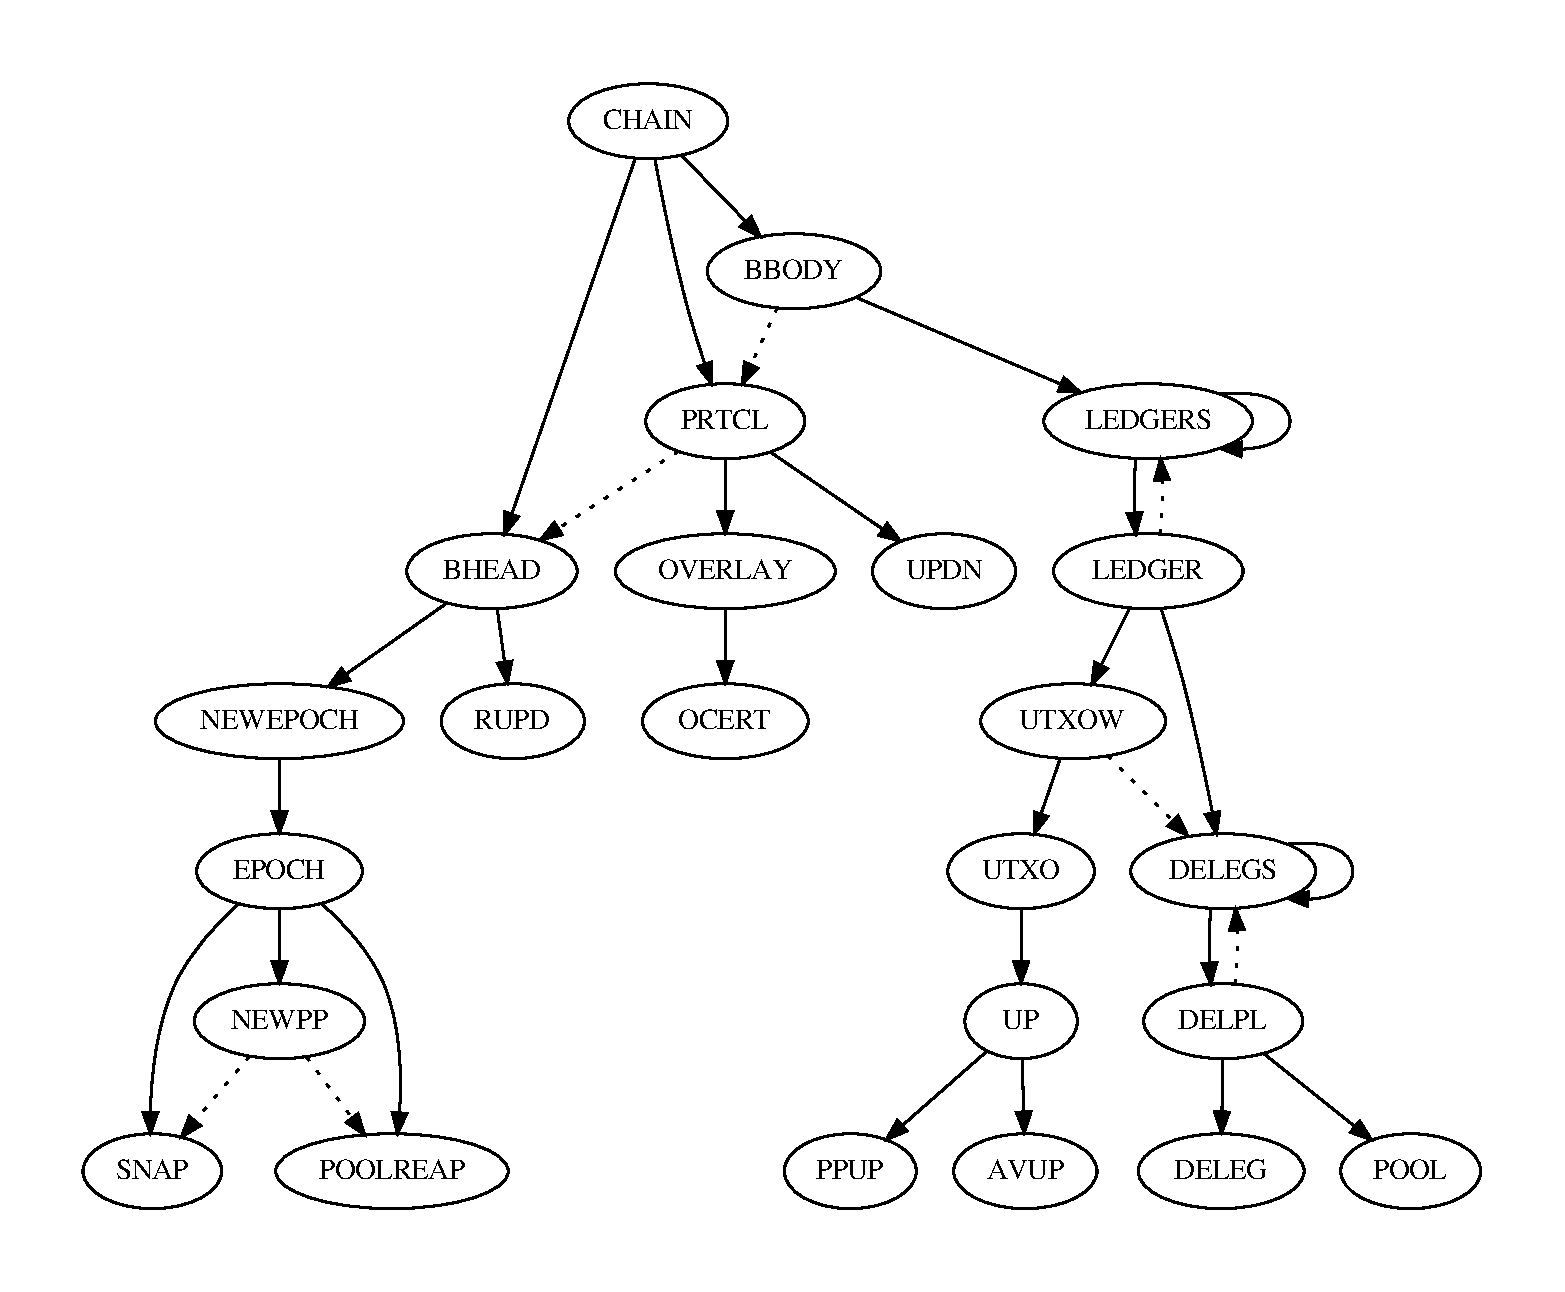
\includegraphics[width=\textwidth]{rules}
  \caption{STS Rules, Sub-Rules and Dependencies}
  \label{fig:sts-rules-dependencies}
\end{figure}

%%% Local Variables:
%%% mode: latex
%%% TeX-master: "ledger-spec"
%%% End:

In this section we discuss the properties which we want the ledger to have. One
goal is to include these properties in the executable specification for doing
property-based testing or formal verification.

\subsection{Validity of a Ledger State}
\label{sec:valid-ledg-state}

Many properties only make sense when applied to a valid ledger state. In
informal terms, a valid ledger state $l$ can only be reached when starting from
an initial state $l_{0}$ (genesis state) and only executing state transition
rules as specified in Section~\ref{sec:state-trans-utxo-1} for UTxO or
Section~\ref{sec:delegation} for delegation.

\begin{figure}[ht]
  \centering
  \begin{align*}
    \genesisId & \in & \TxId \\
    \genesisTxOut & \in & \TxOut \\
    \genesisUTxO & \coloneqq & \{\genesisId, \emptyset\} \mapsto \genesisTxOut
    \\
    \ledgerState & \in & \left(
                         \begin{array}{c}
                           \UTxO \\
                           \DPState
                         \end{array}
    \right)\\
               && \\
    \fun{getUTxO} & \in & \ledgerState \to \UTxO \\
    \fun{getUTxO} & \coloneqq & (\var{utxo}, \wcard) \to \var{utxo}
  \end{align*}
  \caption{Definitions and Functions for Valid Ledger State}
  \label{fig:valid-ledger}
\end{figure}

In Figure~\ref{fig:valid-ledger} \genesisId{} marks the transaction identifier
of the initial coin distribution, where \genesisTxOut{} represents the initial
UTxO. It should be noted that no corresponding inputs exists, i.e., the
transaction inputs are the empty set for the initial transaction. An element of
\ledgerState{} is a tuple of UTxO and delegation witness state (\DPState).

\begin{definition}[\textbf{Valid Ledger State}]
  \begin{multline*}
    \forall l_{0},\ldots,l_{n} \in \ledgerState, l_{0} =
    \left(
      \begin{array}{c}
        \left\{
        \genesisUTxO
        \right\} \\
        \left(
        \begin{array}{c}
          \emptyset\\
          \emptyset
        \end{array}
        \right)
      \end{array}
    \right)  \\
    \implies \forall 0 < i \leq n, (\exists tx_{i} \in \Tx, l_{i-1}
    \trans{ledger}{tx_{i}} l_{i}) \implies \applyFun{validLedgerState} l_{n}
  \end{multline*}
  \label{def:valid-ledger-state}
\end{definition}

Definition~\ref{def:valid-ledger-state} defines a valid ledger state reachable
from the genesis state via valid UTxO, stake delegation or stake pool
transactions. This gives a constructive rule how to reach a valid ledger state.

\subsection{Ledger Properties}
\label{sec:ledger-properties}

The following properties state the desired features of updating a valid ledger
state.

\begin{property}[\textbf{Preserve Balance Modulo Fee}]
  \begin{multline*}
    \forall \var{l}, \var{l'} \in \ledgerState: \applyFun{validLedgerstate}{l}\\
    \implies \forall \var{tx} \in \Tx, \var{l} \trans{utxow}{tx} \var{l'} \\
    \implies \applyFun{destroyed}{pc utxo stKeys rewards tx} =
    \applyFun{created}{pc stPools tx}
  \end{multline*}
  \label{prop:ledger-properties-1}
\end{property}

Property~\ref{prop:ledger-properties-1} states that for each valid ledger $l$,
if a transaction $tx$ is added to the ledger via the state transition rule
$utxow$ to the new ledger state $l'$, the balance of the UTxOs in $l$ equals the
balance of the UTxOs in $l'$ in the sense that the amount of created value in
$l'$ equals the amount of destroyed value in $l$. This means that the total
amount of value is left unchanged by a transaction.

\begin{property}[\textbf{Preserve Balance Restricted to TxIns in Balance of
    TxOuts}]
  \begin{multline*}
    \forall \var{l}, \var{l'} \in \ledgerState: \applyFun{validLedgerstate}{l}\\
    \implies \forall \var{tx} \in \Tx, \var{l} \trans{utxow}{tx} \var{l'}
    \implies \fun{balance}(\applyFun{txins}{tx} \restrictdom
    \applyFun{getUTxO}{l}) = \fun{balance}(\applyFun{outs}{tx}) +
    \applyFun{txfee}{tx}
  \end{multline*}
  \label{prop:ledger-properties-2}
\end{property}

Property~\ref{prop:ledger-properties-2} states the more detailed relation of the
balances change. For ledgers $l, l'$ and a transaction $tx$ as above, the
balance of the UTxOs of $l$ restricted to those whose domain is in the set of
transaction inputs of $tx$ equals the balance of the transaction outputs of $tx$
minus the transaction fees.

\begin{property}[\textbf{Preserve Outputs of Transaction}]
  \begin{multline*}
    \forall \var{l}, \var{l'} \in \ledgerState: \applyFun{validLedgerstate}{l}\\
    \implies \forall \var{tx} \in \Tx, \var{l} \trans{utxow}{tx} \var{l'}
    \implies \forall \var{out} \in \applyFun{outs}{tx}, out \in
    \applyFun{getUTxO}{l'}
  \end{multline*}
  \label{prop:ledger-properties-3}
\end{property}

Property~\ref{prop:ledger-properties-3} states that for every ledger states
$l, l'$ and transaction $tx$ as above, all output UTxOs of $tx$ are in the UTxO
set of $l'$, i.e., they are now available as unspent transaction output.

\begin{property}[\textbf{Eliminate Inputs of Transaction}]
  \begin{multline*}
    \forall \var{l}, \var{l'} \in \ledgerState: \applyFun{validLedgerstate}{l}\\
    \implies \forall \var{tx} \in \Tx, \var{l} \trans{utxow}{tx} \var{l'}
    \implies \forall \var{in} \in \applyFun{txins}{tx}, in \not\in
    \fun{dom}(\applyFun{getUTxO}{l'})
  \end{multline*}
  \label{prop:ledger-properties-4}
\end{property}

Property~\ref{prop:ledger-properties-4} states that for every ledger states
$l, l'$ and transaction $tx$ as above, all transaction inputs $in$ of $tx$ are
not in the domain of the UTxO set of $l'$, i.e., these are no longer available
to spend.

\begin{property}[\textbf{Completeness and Collision-Freeness of new Transaction
    Ids}]
  \begin{multline*}
    \forall \var{l}, \var{l'} \in \ledgerState: \applyFun{validLedgerstate}{l}\\
    \implies \forall \var{tx} \in \Tx, \var{l} \trans{utxow}{tx} \var{l'}
    \implies \forall utxo' \in \applyFun{outs}{tx}, \var{utxo'} \in
    \applyFun{getUTxO}{l'} \wedge \\(\var{utxo'} = ((\var{txId'}, \wcard) \mapsto
    \wcard) \implies \forall \var{utxo} \in \applyFun{getUTxO}{l}, \var{utxo} =
    ((\var{txId}, \wcard) \mapsto \wcard) \implies \var{txId'} \neq \var{txId}
  \end{multline*}
  \label{prop:ledger-properties-5}
\end{property}

Property~\ref{prop:ledger-properties-5} states that for ledger states $l, l'$
and a transaction $tx$ as above, the UTxOs of $l'$ contain all newly created
UTxOs and the referred transaction id of each new UTxO is not used in the UTxO
set of $l$.

\begin{property}[\textbf{Absence of Double-Spend}]
  \begin{multline*}
    \forall l_{0},\ldots,l_{n} \in \ledgerState, l_{0} =
    \left(
      \begin{array}{c}
        \left\{
        \genesisUTxO
        \right\} \\
        \left(
        \begin{array}{c}
          \emptyset\\
          \emptyset
        \end{array}
        \right)
      \end{array}
    \right) \wedge \applyFun{validLedgerState} l_{n} \\
    \implies \forall 0 < i \leq n, tx_{i} \in \Tx, l_{i-1}
    \trans{ledger}{tx_{i}} l_{i} \wedge \applyFun{validLedgerState} l_{i}
    \\ \implies \forall j < i, \applyFun{txins}{tx_{j}} \cap
    \applyFun{txins}{tx_{i}} = \emptyset
  \end{multline*}
  \label{prop:ledger-properties-no-double-spend}
\end{property}

Property~\ref{prop:ledger-properties-no-double-spend} states that for each valid
ledger state $l_{n}$ reachable from the genesis state, each transaction $t_{i}$
does not share any input with any previous transaction $t_{j}$. This means that
each output of a transition is spent at most once.

\subsection{Ledger State Properties for Delegation Transitions}
\label{sec:ledg-prop-deleg}

\begin{figure}[ht]
  \centering
  \begin{align*}
    \fun{getStKeys} & \in & \ledgerState \to \powerset \HashKey \\
    \fun{getStKeys} & \coloneqq & (\wcard, (\var{stKeys}, \wcard, \wcard),
                                  \wcard) \to \var{stkeys} \\
                    &&\\
    \fun{getRewards} & \in & \ledgerState \to \AddrRWD \mapsto \Coin \\
    \fun{getRewards} & \coloneqq & (\wcard, (\wcard, \var{rewards}, \wcard),
                                   \wcard) \to \var{rewards} \\
                    &&\\
    \fun{getDelegations} & \in & \ledgerState \to \HashKey \mapsto \HashKey \\
    \fun{getDelegations} & \coloneqq & (\wcard, (\wcard, \wcard,
                                       \var{delegations}), \wcard) \to
                                       \var{delegations} \\
                    &&\\
    \fun{getStPools} & \in & \ledgerState \to \HashKey \mapsto \DCertRegPool \\
    \fun{getStPools} & \coloneqq & (\wcard, \wcard,
                                   (\var{stpools}, \wcard)) \to \var{stpools} \\
                    &&\\
    \fun{getRetiring} & \in & \ledgerState \to \HashKey \mapsto \Epoch \\
    \fun{getRetiring} & \coloneqq & (\wcard, \wcard,
                                    (\wcard, \var{retiring})) \to \var{retiring} \\
  \end{align*}
  \caption{Definitions and Functions for Stake Delegation in Ledger States}
  \label{fig:stake-delegation-functions}
\end{figure}


\begin{property}[\textbf{Registered Staking Key with Zero Rewards}]
  \begin{multline*}
    \forall \var{l}, \var{l'} \in \ledgerState: \applyFun{validLedgerstate}{l}\\
    \implies \forall \var{c} \in \DCertRegKey, \var{l} \trans{delegw}{c} \var{l'}
    \implies \applyFun{author}{c} = \var{hk}\\ \implies
    \var{hk} \in \applyFun{getStKeys}{l'} \wedge
    (\applyFun{getRewards}var{rewards})[hk] = 0
  \end{multline*}
  \label{prop:ledger-properties-6}
\end{property}

Property~\ref{prop:ledger-properties-6} states that for each valid ledger state
$l$, if a delegation transaction of type $\DCertRegKey$ is executed, then in the
resulting ledger state $l'$, the set of staking keys of $l'$ includes the key
$hk$ associated with the key registration certificate and the associated reward
is set to 0 in $l'$.

\begin{property}[\textbf{Deregistered Staking Key}]
  \begin{multline*}
    \forall \var{l}, \var{l'} \in \ledgerState: \applyFun{validLedgerstate}{l}\\
    \implies \forall \var{c} \in \DCertDeRegKey, \var{l} \trans{delegw}{c} \var{l'}
    \implies \applyFun{author}{c} = \var{hk}\\ \implies
    \var{hk} \not\in \applyFun{getStKeys}{l'} \wedge
    (\fun{dom}(\applyFun{getRewards}{l'}) \cup
    \fun{dom}(\applyFun{getDelegations}{l'})) \cap \{hk\} = \emptyset
  \end{multline*}
  \label{prop:ledger-properties-7}
\end{property}

Property~\ref{prop:ledger-properties-7} states that for $l, l'$ as above but
with a delegation transition of type $\DCertDeRegKey$, the staking key $hk$
associated with the deregistration certificate is not in the set of staking keys
of $l'$ and is not in the domain of neither the rewards nor the delegation map
of $l'$.

\begin{property}[\textbf{Delegated Stake}]
  \begin{multline*}
    \forall \var{l}, \var{l'} \in \ledgerState: \applyFun{validLedgerstate}{l}\\
    \implies \forall \var{c} \in \DCertDeleg, \var{l} \trans{delegw}{c} \var{l'}
    \implies \applyFun{author}{c} = \var{hk}\\ \implies
    \var{hk} \in \applyFun{getStKeys}{l} \wedge
    (\applyFun{getDelegations}{l'})[hk] = \applyFun{pool}{c}
  \end{multline*}
  \label{prop:ledger-properties-8}
\end{property}

Property~\ref{prop:ledger-properties-8} states that for $l, l'$ as above but
with a delegation transition of type $\DCertDeleg$, the staking key $hk$
associated with the deregistration certificate is in the set of staking keys of
$l$ and delegates to the staking pool associated with the delegation
certificate in $l'$.

\subsection{Ledger State Properties for Staking Pool Transitions}
\label{sec:ledg-state-prop}

\begin{property}[\textbf{Registered Staking Pool}]
  \begin{multline*}
    \forall \var{l}, \var{l'} \in \ledgerState: \applyFun{validLedgerstate}{l}\\
    \implies \forall \var{c} \in \DCertRegPool, \var{l} \trans{pool}{c} \var{l'}
    \implies \applyFun{author}{c} = \var{hk}\\ \implies
    (\applyFun{getStPools}{l'})[\var{hk}] = c \wedge \var{hk} \not\in
    \applyFun{getRetiring}{l'}
  \end{multline*}
  \label{prop:ledger-properties-9}
\end{property}

Property~\ref{prop:ledger-properties-9} states that for $l, l'$ as above but
with a delegation transition of type $\DCertRegPool$, the key $hk$ is associated
with the author of the pool registration certificate in $\var{stpools}$ of $l'$
and that $hk$ is not in the set of retiring stake pools in $l'$.

\begin{property}[\textbf{Start Staking Pool Retirement}]
  \begin{multline*}
    \forall \var{l}, \var{l'} \in \ledgerState, \var{cepoch} \in \Epoch:
    \applyFun{validLedgerstate}{l} \\
    \implies \forall \var{c} \in \DCertRetirePool, \var{l} \trans{pool}{c} \var{l'}
    \\ \implies e = \applyFun{retire}{c} \wedge
    \var{cepoch} < e < \var{cepoch} + \emax \wedge \applyFun{author}{c} =
    \var{hk}\\ \implies (\applyFun{getRetiring}{l'})[\var{hk}] = e \wedge
    \var{hk} \in \fun{dom}(\applyFun{getStPools}{l})
  \end{multline*}
  \label{prop:ledger-properties-10}
\end{property}

Property~\ref{prop:ledger-properties-10} states that for $l, l'$ as above but
with a delegation transition of type $\DCertRetirePool$, the key $hk$ is
associated with the author of the pool registration certificate in
$\var{stpools}$ of $l'$ and that $hk$ is not in the set of retiring stake pools
in $l'$.

\begin{property}[\textbf{Stake Pool Reaping}]
  \begin{multline*}
    \forall \var{l}, \var{l'} \in \ledgerState, \var{cepoch} \in \Epoch:
    \applyFun{validLedgerstate}{l} \\
    \implies \var{l} \trans{poolreap}{} \var{l'} \implies \forall \var{retire} =
    retiring^{-1} cepoch, retired \neq \emptyset \\ \wedge \var{retire}
    \subseteq \fun{dom}(\applyFun{getStPool}{l}) \wedge
    \var{retire} \cap \fun{dom}(\applyFun{getStPool}{l'}) = \emptyset \\
    \wedge \var{retire} \subseteq \fun{dom}(\applyFun{getRetiring}{l}) \wedge
    \var{retire} \cap \fun{dom}(\applyFun{getRetiring}{l'}) = \emptyset
  \end{multline*}
  \label{prop:ledger-properties-11}
\end{property}

Property~\ref{prop:ledger-properties-11} states that for $l, l'$ as above but
with a delegation transition of type $\DPoolReap$, there exist registered stake
pools in $l$ which are associated to stake pool registration certificates and
which are to be retired at the current epoch $\var{cepoch}$. In $l'$ all those
stake pools are removed from the maps $stpools$ and $retiring$.


\subsection{Properties of Numerical Calculations}
\label{sec:prop-numer-calc}

The numerical calculations for refunds and rewards calculation in
(see Section~\ref{sec:epoch}) are also required to have certain properties. In
particular we need to make sure that the functions that use non-integral
arithmetic have properties which guarantee consistency of the system. Here, we
state those properties and formulate them in a way that makes them possible to
use properties-based testing for validation in the executable spec.

\begin{property}[\textbf{Minimal Refund}]
  \label{prop:minimal-refund}

  The function $\fun{refund}$ takes a value, a minimal percentage, a decay
  parameter and a duration. It must guarantee that the refunded amount is within
  the minimal refund (off-by-one for rounding / floor) and the original value.

  \begin{multline*}
    \forall d_{val} \in \mathbb{N}, d_{min} \in [0,1], \lambda \in (0, \infty),
    \delta \in \mathbb{N} \\
    \implies \max(0,d_{val}\cdot d_{min} - 1) \leq \floor*{d_{val}\cdot(d_{min} +
      (1-d_{min})\cdot e^{-\lambda\cdot\delta})} \leq d_{val}
  \end{multline*}
\end{property}


\begin{property}[\textbf{Exponential Moving Average}]
  \label{prop:exponential-moving-average}

  The function $\fun{movingAvg}$ calculates the exponential moving average,
  dividing the number of blocks created by the pool by the expected number of
  slots the pool is elected leader (or 1 if the expected number is below 1). It
  guarantees that the result is (i) non-negative and (ii) if a previous moving
  average has already been calculated, the new moving average lies between the
  minimum and maximum of the old and new calculated value. With
  $current := \frac{n}{\max(\overline{N}, 1)}$ this is trivial for (i), for (ii)
  it is

  \begin{multline*}
    \forall \alpha \in [0, 1], n \in \mathbb{N}, \overline{N} \in \Rnn, prev \in
    \Rnn\\
    \implies 0\leq \min(prev, current) \leq
    \alpha\cdot current + (1 - \alpha)\cdot prev
    \leq \max(prev, current)
  \end{multline*}
\end{property}

\begin{property}[\textbf{Actual Reward}]
  \label{prop:actual-reward}

  The actual reward for a stake pool in an epoch is calculated by the function
  $\fun{poolReward}$. The actual reward per stake pool is non-negative and
  bounded by the maximal reward for the stake pool, with $avg$ being the
  calculated moving average of the stake pool and $maxP$ being the maximal
  reward for the stake pool, we get:

  \begin{equation*}
    \forall \gamma \in [0,1] \implies 0\leq \floor*{avg^{\gamma}\cdot maxP} \leq maxP
  \end{equation*}
\end{property}

\begin{todo}
  The property~(\ref{prop:actual-reward}) requires that $avg \in [0,1]$, else
  the actual reward can exceed the maximal reward. This is not true, we need to
  take into account the rewards for all stake pools.
\end{todo}


%%% Local Variables:
%%% mode: latex
%%% TeX-master: "ledger-spec"
%%% End:

\section{Non-Integral Calculations}
\label{sec:non-integr-calc}

In the ledger there are several cases where non-integral calculations are
required, particularly calculations relating to delegation transitions.

\subsection{Types of Non-Integral Calculations}
\label{sec:types-non-integral}

The specification employs non-integral calculations for different mathematical
operations. Table~\ref{tab:func-non-integral} shows the function and transition
rules that use non-integral calculations and which type.

\begin{table}[ht]
  \centering
  \begin{tabular}{lccccc}
    \toprule
    name & page & multiplication & division & exponential function & exponentiation \\
    \midrule
    \fun{refund}
         & \pageref{fig:functions:deposits-refunds} & \checkmark & & \checkmark & \\
    \fun{maxPool}
         & \pageref{fig:functions:rewards} & \checkmark & \checkmark && \\
    \fun{poolReward}
         & \pageref{fig:functions:rewards} & \checkmark & & \checkmark &
                                                                         \checkmark \\
    \fun{r_{leader}}
         & \pageref{fig:functions:reward-splitting} & \checkmark & \checkmark &&\\
         \fun{r_{member}}
         & \pageref{fig:functions:reward-splitting} & \checkmark & \checkmark
                                            &&\\
    \fun{rewardOnePool}
         & \pageref{fig:funcs:epoch-helper} & \checkmark & \checkmark &&\\
    \fun{REWARD}
         &\pageref{fig:rules:reward-update} & \checkmark &&& \\
    \bottomrule
  \end{tabular}
  \caption{Functions with Non-Integral Calculation}
  \label{tab:func-non-integral}
\end{table}

The transcendental exponential function is used in reward and refund calculation
to model the decay of the deposit values. The pool reward uses exponentiation to
calculate a pool's ranking.

The domain for the exponential function are the non-negative reals, more
precisely the distribution parameter $\lambda \in (0, \infty)$ multiplied by a
discrete non-negative duration $\delta$.

The domain of the base of the exponentiation in $\fun{poolReward}$ are the
non-negative reals resulting from the calculation in $\fun{movingAvg}$, the
exponent $\gamma$ is a constant taken from the protocol parameters.

\subsection{Implementation of Non-Integer Calculations}
\label{sec:impl-non-integ}

The large part consists of multiplication and division which can easily be done
using fractional arithmetic to the desired precision. The precision necessary is
bounded by the ability to represent a single lovelace in all calculations.

\subsubsection{Function Simplification}
\label{sec:funct-simpl}

The transcendental function $e^{x}$ can be approximated using different
approaches, depending on the desired accuracy. In general, one uses the
exponential laws $e^{x} = 1/e^{-x}$ and
$e^{x} = \left(e^{\frac{x}{n}} \right)^{n}, n \in \mathbb{N}$ to reduce the
approximation to the unit interval and apply fast integral exponentiation
afterwards.

Exponentiation is implemented using the law
$a^{b} = e^{\ln(a^{b})}= e^{b\ln(a)}$. This therefore requires being able to
calculate $e^{x}$ and $\ln(x)$. The approximation of the natural logarithm can
be approximated using different approaches, again, depending on the desired
accuracy. Most approximations work for $\ln(x), x \in [1, c)$ with some $c >
0$. One then uses the law $\log_{b}(x) = \log_{b}(\frac{x}{b^{n}}b^{n})$ where
$n \in \mathbb{N}$ is chosen in such a way that $\frac{x}{b^{n}} \in [1,
c)$. Using this, one can separate the calculation of the integral and decimal
part as follows:

\begin{equation*}
  \log_{b}(\frac{x}{b^{n}}b^{n})=\log_{b}(b^{n}) + \log_{b}(\frac{x}{b^{n}})=
  n + \log(\frac{x}{b^{n}})
\end{equation*}

\subsubsection{Properties of Function Approximation}
\label{sec:prop-funct-appr-1}

There are several properties that approximations of the transcendental functions
are expected to have. In the following let $\ln'(x)$ be the approximation of
$\ln(x)$, $\exp'(x)$ be the approximation of $e^{x}$ and $x\star y$ the approximation
of $x^{y}$.

\begin{property}[\textbf{monotonicity}]
  \label{prop:monotone}
  Both $\exp'$ and $\ln'$ must be monotone on their respective domains.
\end{property}

In order to guarantee correctness of the approximations, we also require that
the mathematical laws are fulfilled. For some small $\epsilon > 0$, define
$x \approx y \Leftrightarrow \lvert x - y\rvert < \epsilon$.

\begin{property}[\textbf{Mathematical Laws}]
  \label{prop:ln-laws}
  The following mathematical laws state the requirements for the approximations
  of the $\ln'$ and $\exp'$ function:
  \begin{itemize}
  \item $\ln'(x\cdot y) \approx \ln'(x) + \ln'(y)$
  \item $\ln'(x^{y}) \approx y\cdot \ln'(x)$
  \item $\ln'(\exp'(x)) \approx \exp'(\ln'(x)) \approx x$
  \item $x, y \in [0,1] \implies x \star y \in [0, 1]$
  \item $x, y, z \in [0,1], x > 0 \implies
    (z\star\frac{1}{x})\star y \approx (z\star y)\star\frac{1}{x}$
  \item $\exp'(x + y) = \exp'(x) + \exp'(y)$
  \end{itemize}
\end{property}

%%% Local Variables:
%%% mode: latex
%%% TeX-master: "ledger-spec"
%%% End:


\newpage

\begin{appendix}
  \section{Proofs}
\label{sec:proofs}

\newif\ifproofs
% \proofstrue comment in to include generated proofs

For the proofs we use the automated theorem prover
MetiTarski~\cite{DBLP:journals/jar/AkbarpourP10} which is specialized for proofs
over real arithmetic, including elementary functions.

\begin{proof}
The property~(\ref{prop:minimal-refund}) (p.~\pageref{prop:minimal-refund}) for
the minimal refund can be proven automatically via

\begin{verbatim}
fof(minimal_refund, conjecture,
! [Dmin, Lambda, Delta, Dval] :
((Dmin : (=0,1=) & Lambda > 0 & Delta > 0 & Dval > 0
=>
Dval*Dmin >= 0 &
(Dval * (Dmin + (1 - Dmin) * exp(-Lambda * Delta))) : (=Dval * Dmin, Dval=)))).

fof(floor_lower_upper, conjecture,
! [X] :
(X >= 0 => X - 1 <= floor(X) & floor(X) <= X)).
\end{verbatim}
  \verb|minimal_refund| shows that the resulting value is within the interval
  $[d_{val}\cdot d_{min}, d_{val}]$ and that $d_{val}\cdot d_{min}$ is
  non-negative, while \verb|floor_lower_upper| shows that the floor of a value
  $x$ has an upper bound $x$ and lower bound $x - 1$.

\ifproofs
\begin{verbatim}
SZS output start CNFRefutation for minRefund.tptp
cnf(lgen_le_neg, axiom, (X <= Y | ~ lgen(0, X, Y))).

cnf(leq_left_divide_mul_pos, axiom, (Y * Z < X | X / Z <= Y | Z <= 0)).

cnf(interval_intro, axiom,
    (~ lgen(R, A, X) | ~ lgen(S, X, B) | interval(R, A, S, B, X))).

cnf(interval_elim1, axiom, (~ interval(R, A, S, B, X) | lgen(R, A, X))).

cnf(interval_elim2, axiom, (~ interval(R, A, S, B, X) | lgen(S, X, B))).

cnf(exp_upper_bound_cf2, axiom,
    (0 <= X | ~ lgen(R, (X ^ 2 + 6 * X + 12) / (X ^ 2 - 6 * X + 12), Y) |
     lgen(R, exp(X), Y))).

fof(minimal_refund, conjecture,
    (! [Dmin, Lambda, Delta, Dval] :
       ((interval(0, 0, 0, 1, Dmin) & 0 < Lambda & 0 < Delta & 0 < Dval) =>
        (0 <= Dval * Dmin &
         interval(0, Dval * Dmin, 0, Dval,
                  Dval * (Dmin + (1 - Dmin) * exp(-Lambda * Delta))))))).

fof(subgoal_0, plain,
    (! [Dmin, Lambda, Delta, Dval] :
       ((interval(0, 0, 0, 1, Dmin) & 0 < Lambda & 0 < Delta & 0 < Dval) =>
        0 <= Dval * Dmin)), inference(strip, [], [minimal_refund])).

fof(subgoal_1, plain,
    (! [Dmin, Lambda, Delta, Dval] :
       (((interval(0, 0, 0, 1, Dmin) & 0 < Lambda & 0 < Delta & 0 < Dval) &
         0 <= Dval * Dmin) =>
        interval(0, Dval * Dmin, 0, Dval,
                 Dval * (Dmin + (1 - Dmin) * exp(-Lambda * Delta))))),
    inference(strip, [], [minimal_refund])).

fof(negate_0_0, plain,
    (~ ! [Dmin, Lambda, Delta, Dval] :
         ((interval(0, 0, 0, 1, Dmin) & 0 < Lambda & 0 < Delta &
           0 < Dval) => 0 <= Dval * Dmin)),
    inference(negate, [], [subgoal_0])).

fof(normalize_0_0, plain,
    (? [Delta, Dmin, Dval, Lambda] :
       (0 < Delta & 0 < Dval & 0 < Lambda & Dval * Dmin < 0 &
        interval(0, 0, 0, 1, Dmin))),
    inference(canonicalize, [], [negate_0_0])).

fof(normalize_0_1, plain,
    (skoDvalC2 * skoDminC2 < 0 & 0 < skoDeltaC2 & 0 < skoDvalC2 &
     0 < skoLambdaC2 & interval(0, 0, 0, 1, skoDminC2)),
    inference(skolemize, [], [normalize_0_0])).

fof(normalize_0_2, plain, (interval(0, 0, 0, 1, skoDminC2)),
    inference(conjunct, [], [normalize_0_1])).

fof(normalize_0_3, plain, (skoDvalC2 * skoDminC2 < 0),
    inference(conjunct, [], [normalize_0_1])).

fof(normalize_0_4, plain, (0 < skoLambdaC2),
    inference(conjunct, [], [normalize_0_1])).

fof(normalize_0_5, plain, (0 < skoDvalC2),
    inference(conjunct, [], [normalize_0_1])).

fof(normalize_0_6, plain, (0 < skoDeltaC2),
    inference(conjunct, [], [normalize_0_1])).

cnf(refute_0_0, plain, (interval(0, 0, 0, 1, skoDminC2)),
    inference(canonicalize, [], [normalize_0_2])).

cnf(refute_0_1, plain,
    (~ interval(0, 0, 0, 1, skoDminC2) | lgen(0, 0, skoDminC2)),
    inference(subst, [], [interval_elim1])).

cnf(refute_0_2, plain, (lgen(0, 0, skoDminC2)),
    inference(resolve, [], [refute_0_0, refute_0_1])).

cnf(refute_0_3, plain, (0 <= skoDminC2),
    inference(arithmetic, [], [refute_0_2])).

cnf(refute_0_4, plain, (skoDvalC2 * skoDminC2 < 0),
    inference(canonicalize, [], [normalize_0_3])).

cnf(refute_0_5, plain, (0 < skoDvalC2 * (skoDminC2 * -1)),
    inference(arithmetic, [], [refute_0_4])).

cnf(refute_0_6, plain, (0 < skoLambdaC2),
    inference(canonicalize, [], [normalize_0_4])).

cnf(refute_0_7, plain, (0 < skoDvalC2),
    inference(canonicalize, [], [normalize_0_5])).

cnf(refute_0_8, plain, (0 < skoDeltaC2),
    inference(canonicalize, [], [normalize_0_6])).

cnf(refute_0_9, plain, (skoDminC2 < 0),
    inference(decision, [],
              [refute_0_5, refute_0_6, refute_0_7, refute_0_8])).

cnf(refute_0_10, plain, ($false),
    inference(resolve, [], [refute_0_3, refute_0_9])).

fof(negate_1_0, plain,
    (~ ! [Dmin, Lambda, Delta, Dval] :
         (((interval(0, 0, 0, 1, Dmin) & 0 < Lambda & 0 < Delta &
            0 < Dval) & 0 <= Dval * Dmin) =>
          interval(0, Dval * Dmin, 0, Dval,
                   Dval * (Dmin + (1 - Dmin) * exp(-Lambda * Delta))))),
    inference(negate, [], [subgoal_1])).

fof(normalize_1_0, plain,
    (? [Delta, Dmin, Dval, Lambda] :
       (0 < Delta & 0 < Dval & 0 < Lambda &
        ~ interval(0, Dval * Dmin, 0, Dval,
                   Dval * (Dmin + (1 - Dmin) * exp(-Lambda * Delta))) &
        0 <= Dval * Dmin & interval(0, 0, 0, 1, Dmin))),
    inference(canonicalize, [], [negate_1_0])).

fof(normalize_1_1, plain,
    (0 < skoDeltaC3 & 0 < skoDvalC3 & 0 < skoLambdaC3 &
     ~ interval(0, skoDvalC3 * skoDminC3, 0, skoDvalC3,
                skoDvalC3 *
                (skoDminC3 +
                 (1 - skoDminC3) * exp(-skoLambdaC3 * skoDeltaC3))) &
     0 <= skoDvalC3 * skoDminC3 & interval(0, 0, 0, 1, skoDminC3)),
    inference(skolemize, [], [normalize_1_0])).

fof(normalize_1_2, plain,
    (~ interval(0, skoDvalC3 * skoDminC3, 0, skoDvalC3,
                skoDvalC3 *
                (skoDminC3 +
                 (1 - skoDminC3) * exp(-skoLambdaC3 * skoDeltaC3)))),
    inference(conjunct, [], [normalize_1_1])).

fof(normalize_1_3, plain, (interval(0, 0, 0, 1, skoDminC3)),
    inference(conjunct, [], [normalize_1_1])).

fof(normalize_1_4, plain, (0 <= skoDvalC3 * skoDminC3),
    inference(conjunct, [], [normalize_1_1])).

fof(normalize_1_5, plain, (0 < skoLambdaC3),
    inference(conjunct, [], [normalize_1_1])).

fof(normalize_1_6, plain, (0 < skoDvalC3),
    inference(conjunct, [], [normalize_1_1])).

fof(normalize_1_7, plain, (0 < skoDeltaC3),
    inference(conjunct, [], [normalize_1_1])).

cnf(refute_1_0, plain,
    (1 *
     (12 +
      skoLambdaC3 *
      (skoDeltaC3 * 6 + skoLambdaC3 * (skoDeltaC3 * skoDeltaC3))) <
     12 +
     skoLambdaC3 *
     (skoDeltaC3 * -6 + skoLambdaC3 * (skoDeltaC3 * skoDeltaC3)) |
     12 +
     skoLambdaC3 *
     (skoDeltaC3 * 6 + skoLambdaC3 * (skoDeltaC3 * skoDeltaC3)) <= 0 |
     (12 +
      skoLambdaC3 *
      (skoDeltaC3 * -6 + skoLambdaC3 * (skoDeltaC3 * skoDeltaC3))) /
     (12 +
      skoLambdaC3 *
      (skoDeltaC3 * 6 + skoLambdaC3 * (skoDeltaC3 * skoDeltaC3))) <= 1),
    inference(subst, [], [leq_left_divide_mul_pos])).

cnf(refute_1_1, plain,
    (~ lgen(0, exp(X_000190), X_000191) | exp(X_000190) <= X_000191),
    inference(subst, [], [lgen_le_neg])).

cnf(refute_1_2, plain,
    (~ lgen(0,
            (X_000190 ^ 2 + 6 * X_000190 + 12) /
            (X_000190 ^ 2 - 6 * X_000190 + 12), X_000191) | 0 <= X_000190 |
     lgen(0, exp(X_000190), X_000191)),
    inference(subst, [], [exp_upper_bound_cf2])).

cnf(refute_1_3, plain,
    (~ lgen(0,
            (X_000190 ^ 2 + 6 * X_000190 + 12) /
            (X_000190 ^ 2 - 6 * X_000190 + 12), X_000191) | 0 <= X_000190 |
     exp(X_000190) <= X_000191),
    inference(resolve, [], [refute_1_2, refute_1_1])).

cnf(refute_1_4, plain,
    (X_000191 <
     (12 + X_000190 * (6 + X_000190)) / (12 + X_000190 * (-6 + X_000190)) |
     0 <= X_000190 | exp(X_000190) <= X_000191),
    inference(arithmetic, [], [refute_1_3])).

cnf(refute_1_5, plain,
    (1 <
     (12 +
      skoLambdaC3 * (skoDeltaC3 * -1) *
      (6 + skoLambdaC3 * (skoDeltaC3 * -1))) /
     (12 +
      skoLambdaC3 * (skoDeltaC3 * -1) *
      (-6 + skoLambdaC3 * (skoDeltaC3 * -1))) |
     0 <= skoLambdaC3 * (skoDeltaC3 * -1) |
     exp(skoLambdaC3 * (skoDeltaC3 * -1)) <= 1),
    inference(subst, [], [refute_1_4])).

cnf(refute_1_6, plain,
    (~ interval(0, skoDvalC3 * skoDminC3, 0, skoDvalC3,
                skoDvalC3 *
                (skoDminC3 +
                 (1 - skoDminC3) * exp(-skoLambdaC3 * skoDeltaC3)))),
    inference(canonicalize, [], [normalize_1_2])).

cnf(refute_1_7, plain,
    (~ interval(0, skoDvalC3 * skoDminC3, 0, skoDvalC3,
                skoDvalC3 * skoDminC3 +
                exp(skoLambdaC3 * (skoDeltaC3 * -1)) *
                (skoDvalC3 * (1 + skoDminC3 * -1)))),
    inference(arithmetic, [], [refute_1_6])).

cnf(refute_1_8, plain,
    (~ lgen(0, skoDvalC3 * skoDminC3,
            skoDvalC3 * skoDminC3 +
            exp(skoLambdaC3 * (skoDeltaC3 * -1)) *
            (skoDvalC3 * (1 + skoDminC3 * -1))) |
     ~ lgen(0,
            skoDvalC3 * skoDminC3 +
            exp(skoLambdaC3 * (skoDeltaC3 * -1)) *
            (skoDvalC3 * (1 + skoDminC3 * -1)), skoDvalC3) |
     interval(0, skoDvalC3 * skoDminC3, 0, skoDvalC3,
              skoDvalC3 * skoDminC3 +
              exp(skoLambdaC3 * (skoDeltaC3 * -1)) *
              (skoDvalC3 * (1 + skoDminC3 * -1)))),
    inference(subst, [], [interval_intro])).

cnf(refute_1_9, plain,
    (~ lgen(0, skoDvalC3 * skoDminC3,
            skoDvalC3 * skoDminC3 +
            exp(skoLambdaC3 * (skoDeltaC3 * -1)) *
            (skoDvalC3 * (1 + skoDminC3 * -1))) |
     ~ lgen(0,
            skoDvalC3 * skoDminC3 +
            exp(skoLambdaC3 * (skoDeltaC3 * -1)) *
            (skoDvalC3 * (1 + skoDminC3 * -1)), skoDvalC3)),
    inference(resolve, [], [refute_1_8, refute_1_7])).

cnf(refute_1_10, plain,
    (0 <
     exp(skoLambdaC3 * (skoDeltaC3 * -1)) *
     (skoDvalC3 * (-1 + skoDminC3)) |
     skoDvalC3 * (1 + skoDminC3 * -1) <
     exp(skoLambdaC3 * (skoDeltaC3 * -1)) *
     (skoDvalC3 * (1 + skoDminC3 * -1))),
    inference(arithmetic, [], [refute_1_9])).

cnf(refute_1_11, plain,
    (0 <
     exp(skoLambdaC3 * (skoDeltaC3 * -1)) *
     (skoDvalC3 * (-1 + skoDminC3)) |
     exp(skoLambdaC3 * (skoDeltaC3 * -1)) *
     (skoDvalC3 * (-1 + skoDminC3)) <= 0),
    introduced(tautology, [assume])).

cnf(refute_1_12, plain,
    (0 < 0 | skoDvalC3 * (-1 + skoDminC3) < 0 |
     0 < skoDvalC3 * (-1 + skoDminC3) |
     exp(skoLambdaC3 * (skoDeltaC3 * -1)) *
     (skoDvalC3 * (-1 + skoDminC3)) <= 0),
    inference(split, [], [refute_1_11])).

cnf(refute_1_13, plain,
    (0 < skoDvalC3 * (-1 + skoDminC3) |
     0 < skoDvalC3 * (1 + skoDminC3 * -1) |
     exp(skoLambdaC3 * (skoDeltaC3 * -1)) *
     (skoDvalC3 * (-1 + skoDminC3)) <= 0),
    inference(arithmetic, [], [refute_1_12])).

cnf(refute_1_14, plain,
    (exp(skoLambdaC3 * (skoDeltaC3 * -1)) <
     0 / (skoDvalC3 * (-1 + skoDminC3)) |
     0 <= skoDvalC3 * (-1 + skoDminC3) |
     exp(skoLambdaC3 * (skoDeltaC3 * -1)) *
     (skoDvalC3 * (-1 + skoDminC3)) <= 0),
    inference(split, [], [refute_1_11])).

cnf(refute_1_15, plain,
    (exp(skoLambdaC3 * (skoDeltaC3 * -1)) *
     (skoDvalC3 * (-1 + skoDminC3)) <= 0 |
     skoDvalC3 * (1 + skoDminC3 * -1) <= 0),
    inference(arithmetic, [], [refute_1_14])).

cnf(refute_1_16, plain,
    (0 < skoDvalC3 * (-1 + skoDminC3) |
     exp(skoLambdaC3 * (skoDeltaC3 * -1)) *
     (skoDvalC3 * (-1 + skoDminC3)) <= 0),
    inference(resolve, [], [refute_1_15, refute_1_13])).

cnf(refute_1_17, plain, (interval(0, 0, 0, 1, skoDminC3)),
    inference(canonicalize, [], [normalize_1_3])).

cnf(refute_1_18, plain,
    (~ interval(0, 0, 0, 1, skoDminC3) | lgen(0, skoDminC3, 1)),
    inference(subst, [], [interval_elim2])).

cnf(refute_1_19, plain, (lgen(0, skoDminC3, 1)),
    inference(resolve, [], [refute_1_17, refute_1_18])).

cnf(refute_1_20, plain, (skoDminC3 <= 1),
    inference(arithmetic, [], [refute_1_19])).

cnf(refute_1_21, plain, (0 <= skoDvalC3 * skoDminC3),
    inference(canonicalize, [], [normalize_1_4])).

cnf(refute_1_22, plain, (skoDvalC3 * (skoDminC3 * -1) <= 0),
    inference(arithmetic, [], [refute_1_21])).

cnf(refute_1_23, plain, (0 < skoLambdaC3),
    inference(canonicalize, [], [normalize_1_5])).

cnf(refute_1_24, plain, (0 < skoDvalC3),
    inference(canonicalize, [], [normalize_1_6])).

cnf(refute_1_25, plain, (0 < skoDeltaC3),
    inference(canonicalize, [], [normalize_1_7])).

cnf(refute_1_26, plain, (skoDvalC3 * (-1 + skoDminC3) <= 0),
    inference(decision, [],
              [refute_1_20, refute_1_22, refute_1_23, refute_1_24,
               refute_1_25])).

cnf(refute_1_27, plain,
    (exp(skoLambdaC3 * (skoDeltaC3 * -1)) *
     (skoDvalC3 * (-1 + skoDminC3)) <= 0),
    inference(resolve, [], [refute_1_26, refute_1_16])).

cnf(refute_1_28, plain,
    (skoDvalC3 * (1 + skoDminC3 * -1) <
     exp(skoLambdaC3 * (skoDeltaC3 * -1)) *
     (skoDvalC3 * (1 + skoDminC3 * -1))),
    inference(resolve, [], [refute_1_27, refute_1_10])).

cnf(refute_1_29, plain,
    (skoDvalC3 * (1 + skoDminC3 * -1) /
     (skoDvalC3 * (1 + skoDminC3 * -1)) <
     exp(skoLambdaC3 * (skoDeltaC3 * -1)) |
     skoDvalC3 * (1 + skoDminC3 * -1) <= 0),
    inference(split, [], [refute_1_28])).

cnf(refute_1_30, plain,
    (1 < exp(skoLambdaC3 * (skoDeltaC3 * -1)) |
     skoDvalC3 * (1 + skoDminC3 * -1) <= 0 | 1 = skoDminC3 |
     skoDvalC3 = 0), inference(arithmetic, [], [refute_1_29])).

cnf(refute_1_31, plain,
    (0 < skoDvalC3 * (1 + skoDminC3 * -1) | 1 = skoDminC3 | skoDvalC3 = 0),
    inference(decision, [],
              [refute_1_25, refute_1_24, refute_1_23, refute_1_22,
               refute_1_20])).

cnf(refute_1_32, plain,
    (1 < exp(skoLambdaC3 * (skoDeltaC3 * -1)) | 1 = skoDminC3 |
     skoDvalC3 = 0), inference(resolve, [], [refute_1_30, refute_1_31])).

cnf(refute_1_33, plain, (skoDvalC3 != 0 | 1 = skoDminC3),
    inference(decision, [],
              [refute_1_25, refute_1_24, refute_1_23, refute_1_22,
               refute_1_20])).

cnf(refute_1_34, plain,
    (1 < exp(skoLambdaC3 * (skoDeltaC3 * -1)) | 1 = skoDminC3),
    inference(resolve, [], [refute_1_32, refute_1_33])).

cnf(refute_1_35, plain,
    (1 <
     (12 +
      skoLambdaC3 * (skoDeltaC3 * -1) *
      (6 + skoLambdaC3 * (skoDeltaC3 * -1))) /
     (12 +
      skoLambdaC3 * (skoDeltaC3 * -1) *
      (-6 + skoLambdaC3 * (skoDeltaC3 * -1))) |
     0 <= skoLambdaC3 * (skoDeltaC3 * -1) | 1 = skoDminC3),
    inference(resolve, [], [refute_1_5, refute_1_34])).

cnf(refute_1_36, plain,
    (1 <
     (12 +
      skoLambdaC3 *
      (skoDeltaC3 * -6 + skoLambdaC3 * (skoDeltaC3 * skoDeltaC3))) /
     (12 +
      skoLambdaC3 *
      (skoDeltaC3 * 6 + skoLambdaC3 * (skoDeltaC3 * skoDeltaC3))) |
     skoLambdaC3 * skoDeltaC3 <= 0 | 1 = skoDminC3),
    inference(arithmetic, [], [refute_1_35])).

cnf(refute_1_37, plain,
    (skoDvalC3 * (1 + skoDminC3 * -1) < 0 |
     0 < skoDvalC3 * (1 + skoDminC3 * -1)),
    inference(split, [], [refute_1_28])).

cnf(refute_1_38, plain,
    (0 < skoDvalC3 * (-1 + skoDminC3) |
     0 < skoDvalC3 * (1 + skoDminC3 * -1)),
    inference(arithmetic, [], [refute_1_37])).

cnf(refute_1_39, plain,
    (0 < skoDvalC3 * (1 + skoDminC3 * -1) |
     skoDvalC3 * (-1 + skoDminC3) <= 0),
    inference(decision, [],
              [refute_1_25, refute_1_24, refute_1_23, refute_1_22,
               refute_1_20])).

cnf(refute_1_40, plain, (0 < skoDvalC3 * (1 + skoDminC3 * -1)),
    inference(resolve, [], [refute_1_39, refute_1_38])).

cnf(refute_1_41, plain, (0 < skoLambdaC3 * skoDeltaC3 | 1 = skoDminC3),
    inference(decision, [],
              [refute_1_40, refute_1_25, refute_1_24, refute_1_23,
               refute_1_22, refute_1_20])).

cnf(refute_1_42, plain,
    (1 <
     (12 +
      skoLambdaC3 *
      (skoDeltaC3 * -6 + skoLambdaC3 * (skoDeltaC3 * skoDeltaC3))) /
     (12 +
      skoLambdaC3 *
      (skoDeltaC3 * 6 + skoLambdaC3 * (skoDeltaC3 * skoDeltaC3))) |
     1 = skoDminC3), inference(resolve, [], [refute_1_36, refute_1_41])).

cnf(refute_1_43, plain, (1 != skoDminC3),
    inference(decision, [],
              [refute_1_40, refute_1_25, refute_1_24, refute_1_23,
               refute_1_22, refute_1_20])).

cnf(refute_1_44, plain,
    (1 <
     (12 +
      skoLambdaC3 *
      (skoDeltaC3 * -6 + skoLambdaC3 * (skoDeltaC3 * skoDeltaC3))) /
     (12 +
      skoLambdaC3 *
      (skoDeltaC3 * 6 + skoLambdaC3 * (skoDeltaC3 * skoDeltaC3)))),
    inference(resolve, [], [refute_1_42, refute_1_43])).

cnf(refute_1_45, plain,
    (1 *
     (12 +
      skoLambdaC3 *
      (skoDeltaC3 * 6 + skoLambdaC3 * (skoDeltaC3 * skoDeltaC3))) <
     12 +
     skoLambdaC3 *
     (skoDeltaC3 * -6 + skoLambdaC3 * (skoDeltaC3 * skoDeltaC3)) |
     12 +
     skoLambdaC3 *
     (skoDeltaC3 * 6 + skoLambdaC3 * (skoDeltaC3 * skoDeltaC3)) <= 0),
    inference(resolve, [], [refute_1_0, refute_1_44])).

cnf(refute_1_46, plain,
    (0 < skoLambdaC3 * (skoDeltaC3 * -12) |
     skoLambdaC3 *
     (skoDeltaC3 * 6 + skoLambdaC3 * (skoDeltaC3 * skoDeltaC3)) <= -12),
    inference(arithmetic, [], [refute_1_45])).

cnf(refute_1_47, plain,
    (0 < skoLambdaC3 * (skoDeltaC3 * -12) |
     -12 <
     skoLambdaC3 *
     (skoDeltaC3 * 6 + skoLambdaC3 * (skoDeltaC3 * skoDeltaC3))),
    inference(decision, [],
              [refute_1_40, refute_1_25, refute_1_24, refute_1_23,
               refute_1_22, refute_1_20])).

cnf(refute_1_48, plain, (0 < skoLambdaC3 * (skoDeltaC3 * -12)),
    inference(resolve, [], [refute_1_46, refute_1_47])).

cnf(refute_1_49, plain, (skoLambdaC3 * (skoDeltaC3 * -12) <= 0),
    inference(decision, [],
              [refute_1_40, refute_1_25, refute_1_24, refute_1_23,
               refute_1_22, refute_1_20])).

cnf(refute_1_50, plain, ($false),
    inference(resolve, [], [refute_1_49, refute_1_48])).
SZS output end CNFRefutation for minRefund.tptp
\end{verbatim}

\begin{verbatim}
SZS output start CNFRefutation for floor.tptp
cnf(lgen_le_neg, axiom, (X <= Y | ~ lgen(0, X, Y))).

cnf(floor_upper_bound, axiom, (~ lgen(R, X, Y) | lgen(R, floor(X), Y))).

cnf(floor_lower_bound, axiom, (X - 1 < Y | lgen(R, Y, floor(X)))).

fof(floor_lower_upper, conjecture,
    (! [X] : (0 <= X => (X - 1 <= floor(X) & floor(X) <= X)))).

fof(subgoal_0, plain, (! [X] : (0 <= X => X - 1 <= floor(X))),
    inference(strip, [], [floor_lower_upper])).

fof(subgoal_1, plain,
    (! [X] : ((0 <= X & X - 1 <= floor(X)) => floor(X) <= X)),
    inference(strip, [], [floor_lower_upper])).

fof(negate_0_0, plain, (~ ! [X] : (0 <= X => X - 1 <= floor(X))),
    inference(negate, [], [subgoal_0])).

fof(normalize_0_0, plain, (? [X] : (floor(X) < X - 1 & 0 <= X)),
    inference(canonicalize, [], [negate_0_0])).

fof(normalize_0_1, plain, (floor(skoXC2) < skoXC2 - 1 & 0 <= skoXC2),
    inference(skolemize, [], [normalize_0_0])).

fof(normalize_0_2, plain, (floor(skoXC2) < skoXC2 - 1),
    inference(conjunct, [], [normalize_0_1])).

cnf(refute_0_0, plain, (floor(skoXC2) < skoXC2 - 1),
    inference(canonicalize, [], [normalize_0_2])).

cnf(refute_0_1, plain, (floor(skoXC2) < -1 + skoXC2),
    inference(arithmetic, [], [refute_0_0])).

cnf(refute_0_2, plain,
    (~ lgen(0, X_000012, floor(X_000011)) | X_000012 <= floor(X_000011)),
    inference(subst, [], [lgen_le_neg])).

cnf(refute_0_3, plain,
    (X_000011 - 1 < X_000012 | lgen(0, X_000012, floor(X_000011))),
    inference(subst, [], [floor_lower_bound])).

cnf(refute_0_4, plain,
    (X_000011 - 1 < X_000012 | X_000012 <= floor(X_000011)),
    inference(resolve, [], [refute_0_3, refute_0_2])).

cnf(refute_0_5, plain,
    (-1 + X_000011 < X_000012 | X_000012 <= floor(X_000011)),
    inference(arithmetic, [], [refute_0_4])).

cnf(refute_0_6, plain,
    (-1 + skoXC2 < -1 + skoXC2 | -1 + skoXC2 <= floor(skoXC2)),
    inference(subst, [], [refute_0_5])).

cnf(refute_0_7, plain, (-1 + skoXC2 < -1 + skoXC2),
    inference(resolve, [], [refute_0_6, refute_0_1])).

cnf(refute_0_8, plain, ($false), inference(arithmetic, [], [refute_0_7])).

fof(negate_1_0, plain,
    (~ ! [X] : ((0 <= X & X - 1 <= floor(X)) => floor(X) <= X)),
    inference(negate, [], [subgoal_1])).

fof(normalize_1_0, plain,
    (? [X] : (X < floor(X) & 0 <= X & X - 1 <= floor(X))),
    inference(canonicalize, [], [negate_1_0])).

fof(normalize_1_1, plain,
    (skoXC3 < floor(skoXC3) & 0 <= skoXC3 & skoXC3 - 1 <= floor(skoXC3)),
    inference(skolemize, [], [normalize_1_0])).

fof(normalize_1_2, plain, (skoXC3 < floor(skoXC3)),
    inference(conjunct, [], [normalize_1_1])).

cnf(refute_1_0, plain, (skoXC3 < floor(skoXC3)),
    inference(canonicalize, [], [normalize_1_2])).

cnf(refute_1_1, plain,
    (~ lgen(0, floor(X_000034), X_000035) | floor(X_000034) <= X_000035),
    inference(subst, [], [lgen_le_neg])).

cnf(refute_1_2, plain,
    (~ lgen(0, X_000034, X_000035) | lgen(0, floor(X_000034), X_000035)),
    inference(subst, [], [floor_upper_bound])).

cnf(refute_1_3, plain,
    (~ lgen(0, X_000034, X_000035) | floor(X_000034) <= X_000035),
    inference(resolve, [], [refute_1_2, refute_1_1])).

cnf(refute_1_4, plain, (X_000035 < X_000034 | floor(X_000034) <= X_000035),
    inference(arithmetic, [], [refute_1_3])).

cnf(refute_1_5, plain, (skoXC3 < skoXC3 | floor(skoXC3) <= skoXC3),
    inference(subst, [], [refute_1_4])).

cnf(refute_1_6, plain, (skoXC3 < skoXC3),
    inference(resolve, [], [refute_1_5, refute_1_0])).

cnf(refute_1_7, plain, ($false), inference(arithmetic, [], [refute_1_6])).
SZS output end CNFRefutation for floor.tptp
\end{verbatim}
\fi
\end{proof}


\begin{proof}
  For the property~(\ref{prop:reward-splitting})
  (p.~\pageref{prop:reward-splitting}) for reward splitting we actually show a
  stronger one, by removing the floor function. Using the fractional values we
  get an upper bound for the real value and showing that this upper bound is
  bounded by $\hat{f}$ we show that the real value is also bounded by
  $\hat{f}$. To eliminate the sum, we use the identity $\frac{s +
    \sum_{j}t_{j}}{\sigma} = 1$, see the definition of
  $\sigma$ in~\cite{delegation_design}. Using this, we show for $\hat{f} > c$

  \begin{equation*}
    \begin{array}{cll}
      & 0 \leq c + (\hat{f} - c)\cdot (m + (1 - m))\cdot \frac{s}{\sigma} +
        \sum_{j}(\hat{f}-c)\cdot(1-m)\cdot\frac{t_{j}}{\sigma} & \leq \hat{f} \\
      \Leftrightarrow &
                        0\leq c + (\hat{f}-c)\cdot m \cdot \frac{s}{\sigma} + (\hat{f}
                        -c)\cdot(1-m)\cdot\frac{s + \sum_{j}t_{j}}{\sigma} & \leq \hat{f} \\
      \Leftrightarrow &
                        0\leq c + (\hat{f}-c)\cdot m \cdot \frac{s}{\sigma} + (\hat{f}
                        -c)\cdot(1-m) & \leq \hat{f} \\
    \end{array}
  \end{equation*}

  This can be proven automatically using

\begin{verbatim}
fof(reward_splitting, conjecture,
! [C, F, M, S, Sigma] :
(
M : (=0, 1=) & C >= 0 & F > C & Sigma : (0, 1=) & S : (=0, Sigma=)
=>
C + (F - C) * M * S / Sigma + (F - C) * (1 - M) <= F &
0 <= C + (F - C) * M * S / Sigma + (F - C) * (1 - M))).
\end{verbatim}

  \ifproofs
\begin{verbatim}
SZS output start CNFRefutation for rewardsplit.tptp
cnf(leq_left_divide_mul_pos, axiom, (Y * Z < X | X / Z <= Y | Z <= 0)).

cnf(leq_right_divide_mul_pos, axiom, (Y < X * Z | X <= Y / Z | Z <= 0)).

cnf(leq_left_divide_mul_neg, axiom, (Y * Z < X | Y <= X / Z | 0 <= Z)).

cnf(leq_right_divide_mul_neg, axiom, (Y < X * Z | Y / Z <= X | 0 <= Z)).

cnf(interval_elim1, axiom, (~ interval(R, A, S, B, X) | lgen(R, A, X))).

cnf(interval_elim2, axiom, (~ interval(R, A, S, B, X) | lgen(S, X, B))).

fof(reward_splitting, conjecture,
    (! [C, F, M, S, Sigma] :
       ((interval(0, 0, 0, 1, M) & 0 <= C & C < F &
         interval(1, 0, 0, 1, Sigma) & interval(0, 0, 0, Sigma, S)) =>
        (C + (F - C) * M * S / Sigma + (F - C) * (1 - M) <= F &
         0 <= C + (F - C) * M * S / Sigma + (F - C) * (1 - M))))).

fof(subgoal_0, plain,
    (! [C, F, M, S, Sigma] :
       ((interval(0, 0, 0, 1, M) & 0 <= C & C < F &
         interval(1, 0, 0, 1, Sigma) & interval(0, 0, 0, Sigma, S)) =>
        C + (F - C) * M * S / Sigma + (F - C) * (1 - M) <= F)),
    inference(strip, [], [reward_splitting])).

fof(subgoal_1, plain,
    (! [C, F, M, S, Sigma] :
       (((interval(0, 0, 0, 1, M) & 0 <= C & C < F &
          interval(1, 0, 0, 1, Sigma) & interval(0, 0, 0, Sigma, S)) &
         C + (F - C) * M * S / Sigma + (F - C) * (1 - M) <= F) =>
        0 <= C + (F - C) * M * S / Sigma + (F - C) * (1 - M))),
    inference(strip, [], [reward_splitting])).

fof(negate_0_0, plain,
    (~ ! [C, F, M, S, Sigma] :
         ((interval(0, 0, 0, 1, M) & 0 <= C & C < F &
           interval(1, 0, 0, 1, Sigma) & interval(0, 0, 0, Sigma, S)) =>
          C + (F - C) * M * S / Sigma + (F - C) * (1 - M) <= F)),
    inference(negate, [], [subgoal_0])).

fof(normalize_0_0, plain,
    (? [C, F, M, S, Sigma] :
       (C < F & F < C + (F - C) * M * S / Sigma + (F - C) * (1 - M) &
        0 <= C & interval(0, 0, 0, Sigma, S) & interval(0, 0, 0, 1, M) &
        interval(1, 0, 0, 1, Sigma))),
    inference(canonicalize, [], [negate_0_0])).

fof(normalize_0_1, plain,
    (skoFC2 <
     skoCC2 + (skoFC2 - skoCC2) * skoMC2 * skoSC2 / skoSigmaC2 +
     (skoFC2 - skoCC2) * (1 - skoMC2) & skoCC2 < skoFC2 & 0 <= skoCC2 &
     interval(0, 0, 0, 1, skoMC2) & interval(0, 0, 0, skoSigmaC2, skoSC2) &
     interval(1, 0, 0, 1, skoSigmaC2)),
    inference(skolemize, [], [normalize_0_0])).

fof(normalize_0_2, plain, (interval(0, 0, 0, skoSigmaC2, skoSC2)),
    inference(conjunct, [], [normalize_0_1])).

fof(normalize_0_3, plain, (interval(1, 0, 0, 1, skoSigmaC2)),
    inference(conjunct, [], [normalize_0_1])).

fof(normalize_0_4, plain, (interval(0, 0, 0, 1, skoMC2)),
    inference(conjunct, [], [normalize_0_1])).

fof(normalize_0_5, plain,
    (skoFC2 <
     skoCC2 + (skoFC2 - skoCC2) * skoMC2 * skoSC2 / skoSigmaC2 +
     (skoFC2 - skoCC2) * (1 - skoMC2)),
    inference(conjunct, [], [normalize_0_1])).

fof(normalize_0_6, plain, (0 <= skoCC2),
    inference(conjunct, [], [normalize_0_1])).

fof(normalize_0_7, plain, (skoCC2 < skoFC2),
    inference(conjunct, [], [normalize_0_1])).

cnf(refute_0_0, plain, (interval(0, 0, 0, skoSigmaC2, skoSC2)),
    inference(canonicalize, [], [normalize_0_2])).

cnf(refute_0_1, plain,
    (~ interval(0, 0, 0, skoSigmaC2, skoSC2) |
     lgen(0, skoSC2, skoSigmaC2)), inference(subst, [], [interval_elim2])).

cnf(refute_0_2, plain, (lgen(0, skoSC2, skoSigmaC2)),
    inference(resolve, [], [refute_0_0, refute_0_1])).

cnf(refute_0_3, plain, (skoSC2 <= skoSigmaC2),
    inference(arithmetic, [], [refute_0_2])).

cnf(refute_0_4, plain, (interval(1, 0, 0, 1, skoSigmaC2)),
    inference(canonicalize, [], [normalize_0_3])).

cnf(refute_0_5, plain,
    (~ interval(1, 0, 0, 1, skoSigmaC2) | lgen(1, 0, skoSigmaC2)),
    inference(subst, [], [interval_elim1])).

cnf(refute_0_6, plain, (lgen(1, 0, skoSigmaC2)),
    inference(resolve, [], [refute_0_4, refute_0_5])).

cnf(refute_0_7, plain, (0 < skoSigmaC2),
    inference(arithmetic, [], [refute_0_6])).

cnf(refute_0_8, plain,
    (~ interval(0, 0, 0, skoSigmaC2, skoSC2) | lgen(0, 0, skoSC2)),
    inference(subst, [], [interval_elim1])).

cnf(refute_0_9, plain, (lgen(0, 0, skoSC2)),
    inference(resolve, [], [refute_0_0, refute_0_8])).

cnf(refute_0_10, plain, (0 <= skoSC2),
    inference(arithmetic, [], [refute_0_9])).

cnf(refute_0_11, plain, (interval(0, 0, 0, 1, skoMC2)),
    inference(canonicalize, [], [normalize_0_4])).

cnf(refute_0_12, plain,
    (~ interval(0, 0, 0, 1, skoMC2) | lgen(0, 0, skoMC2)),
    inference(subst, [], [interval_elim1])).

cnf(refute_0_13, plain, (lgen(0, 0, skoMC2)),
    inference(resolve, [], [refute_0_11, refute_0_12])).

cnf(refute_0_14, plain, (0 <= skoMC2),
    inference(arithmetic, [], [refute_0_13])).

cnf(refute_0_15, plain,
    (skoFC2 <
     skoCC2 + (skoFC2 - skoCC2) * skoMC2 * skoSC2 / skoSigmaC2 +
     (skoFC2 - skoCC2) * (1 - skoMC2)),
    inference(canonicalize, [], [normalize_0_5])).

cnf(refute_0_16, plain,
    (skoMC2 * (skoCC2 * -1 + skoFC2) <
     skoSC2 * (skoMC2 * (skoCC2 * -1 + skoFC2)) / skoSigmaC2),
    inference(arithmetic, [], [refute_0_15])).

cnf(refute_0_17, plain,
    (skoSC2 * (skoMC2 * (skoCC2 * -1 + skoFC2)) <
     skoMC2 * (skoCC2 * -1 + skoFC2) * skoSigmaC2 | 0 <= skoSigmaC2 |
     skoSC2 * (skoMC2 * (skoCC2 * -1 + skoFC2)) / skoSigmaC2 <=
     skoMC2 * (skoCC2 * -1 + skoFC2)),
    inference(subst, [], [leq_right_divide_mul_neg])).

cnf(refute_0_18, plain,
    (skoSC2 * (skoMC2 * (skoCC2 * -1 + skoFC2)) <
     skoMC2 * (skoCC2 * -1 + skoFC2) * skoSigmaC2 | 0 <= skoSigmaC2),
    inference(resolve, [], [refute_0_17, refute_0_16])).

cnf(refute_0_19, plain,
    (skoSC2 * (skoMC2 * (skoCC2 * -1 + skoFC2)) <
     skoSigmaC2 * (skoMC2 * (skoCC2 * -1 + skoFC2)) | 0 <= skoSigmaC2),
    inference(arithmetic, [], [refute_0_18])).

cnf(refute_0_20, plain,
    (skoMC2 * (skoCC2 * -1 + skoFC2) * skoSigmaC2 <
     skoSC2 * (skoMC2 * (skoCC2 * -1 + skoFC2)) |
     skoSC2 * (skoMC2 * (skoCC2 * -1 + skoFC2)) / skoSigmaC2 <=
     skoMC2 * (skoCC2 * -1 + skoFC2) | skoSigmaC2 <= 0),
    inference(subst, [], [leq_left_divide_mul_pos])).

cnf(refute_0_21, plain,
    (skoMC2 * (skoCC2 * -1 + skoFC2) * skoSigmaC2 <
     skoSC2 * (skoMC2 * (skoCC2 * -1 + skoFC2)) | skoSigmaC2 <= 0),
    inference(resolve, [], [refute_0_20, refute_0_16])).

cnf(refute_0_22, plain,
    (skoSC2 * (skoMC2 * (skoCC2 + skoFC2 * -1)) <
     skoSigmaC2 * (skoMC2 * (skoCC2 + skoFC2 * -1)) | skoSigmaC2 <= 0),
    inference(arithmetic, [], [refute_0_21])).

cnf(refute_0_23, plain, (0 <= skoCC2),
    inference(canonicalize, [], [normalize_0_6])).

cnf(refute_0_24, plain, (skoCC2 < skoFC2),
    inference(canonicalize, [], [normalize_0_7])).

cnf(refute_0_25, plain, (skoSigmaC2 < skoSC2),
    inference(decision, [],
              [refute_0_7, refute_0_10, refute_0_14, refute_0_19,
               refute_0_22, refute_0_23, refute_0_24])).

cnf(refute_0_26, plain, ($false),
    inference(resolve, [], [refute_0_3, refute_0_25])).

fof(negate_1_0, plain,
    (~ ! [C, F, M, S, Sigma] :
         (((interval(0, 0, 0, 1, M) & 0 <= C & C < F &
            interval(1, 0, 0, 1, Sigma) & interval(0, 0, 0, Sigma, S)) &
           C + (F - C) * M * S / Sigma + (F - C) * (1 - M) <= F) =>
          0 <= C + (F - C) * M * S / Sigma + (F - C) * (1 - M))),
    inference(negate, [], [subgoal_1])).

fof(normalize_1_0, plain,
    (? [C, F, M, S, Sigma] :
       (C < F & C + (F - C) * M * S / Sigma + (F - C) * (1 - M) < 0 &
        0 <= C & C + (F - C) * M * S / Sigma + (F - C) * (1 - M) <= F &
        interval(0, 0, 0, Sigma, S) & interval(0, 0, 0, 1, M) &
        interval(1, 0, 0, 1, Sigma))),
    inference(canonicalize, [], [negate_1_0])).

fof(normalize_1_1, plain,
    (skoCC3 + (skoFC3 - skoCC3) * skoMC3 * skoSC3 / skoSigmaC3 +
     (skoFC3 - skoCC3) * (1 - skoMC3) < 0 & skoCC3 < skoFC3 & 0 <= skoCC3 &
     skoCC3 + (skoFC3 - skoCC3) * skoMC3 * skoSC3 / skoSigmaC3 +
     (skoFC3 - skoCC3) * (1 - skoMC3) <= skoFC3 &
     interval(0, 0, 0, 1, skoMC3) & interval(0, 0, 0, skoSigmaC3, skoSC3) &
     interval(1, 0, 0, 1, skoSigmaC3)),
    inference(skolemize, [], [normalize_1_0])).

fof(normalize_1_2, plain, (interval(0, 0, 0, 1, skoMC3)),
    inference(conjunct, [], [normalize_1_1])).

fof(normalize_1_3, plain, (interval(1, 0, 0, 1, skoSigmaC3)),
    inference(conjunct, [], [normalize_1_1])).

fof(normalize_1_4, plain, (interval(0, 0, 0, skoSigmaC3, skoSC3)),
    inference(conjunct, [], [normalize_1_1])).

fof(normalize_1_5, plain,
    (skoCC3 + (skoFC3 - skoCC3) * skoMC3 * skoSC3 / skoSigmaC3 +
     (skoFC3 - skoCC3) * (1 - skoMC3) < 0),
    inference(conjunct, [], [normalize_1_1])).

fof(normalize_1_6, plain, (0 <= skoCC3),
    inference(conjunct, [], [normalize_1_1])).

fof(normalize_1_7, plain, (skoCC3 < skoFC3),
    inference(conjunct, [], [normalize_1_1])).

cnf(refute_1_0, plain, (interval(0, 0, 0, 1, skoMC3)),
    inference(canonicalize, [], [normalize_1_2])).

cnf(refute_1_1, plain,
    (~ interval(0, 0, 0, 1, skoMC3) | lgen(0, skoMC3, 1)),
    inference(subst, [], [interval_elim2])).

cnf(refute_1_2, plain, (lgen(0, skoMC3, 1)),
    inference(resolve, [], [refute_1_0, refute_1_1])).

cnf(refute_1_3, plain, (skoMC3 <= 1),
    inference(arithmetic, [], [refute_1_2])).

cnf(refute_1_4, plain, (interval(1, 0, 0, 1, skoSigmaC3)),
    inference(canonicalize, [], [normalize_1_3])).

cnf(refute_1_5, plain,
    (~ interval(1, 0, 0, 1, skoSigmaC3) | lgen(1, 0, skoSigmaC3)),
    inference(subst, [], [interval_elim1])).

cnf(refute_1_6, plain, (lgen(1, 0, skoSigmaC3)),
    inference(resolve, [], [refute_1_4, refute_1_5])).

cnf(refute_1_7, plain, (0 < skoSigmaC3),
    inference(arithmetic, [], [refute_1_6])).

cnf(refute_1_8, plain, (interval(0, 0, 0, skoSigmaC3, skoSC3)),
    inference(canonicalize, [], [normalize_1_4])).

cnf(refute_1_9, plain,
    (~ interval(0, 0, 0, skoSigmaC3, skoSC3) | lgen(0, 0, skoSC3)),
    inference(subst, [], [interval_elim1])).

cnf(refute_1_10, plain, (lgen(0, 0, skoSC3)),
    inference(resolve, [], [refute_1_8, refute_1_9])).

cnf(refute_1_11, plain, (0 <= skoSC3),
    inference(arithmetic, [], [refute_1_10])).

cnf(refute_1_12, plain,
    (~ interval(0, 0, 0, 1, skoMC3) | lgen(0, 0, skoMC3)),
    inference(subst, [], [interval_elim1])).

cnf(refute_1_13, plain, (lgen(0, 0, skoMC3)),
    inference(resolve, [], [refute_1_0, refute_1_12])).

cnf(refute_1_14, plain, (0 <= skoMC3),
    inference(arithmetic, [], [refute_1_13])).

cnf(refute_1_15, plain,
    (skoCC3 + (skoFC3 - skoCC3) * skoMC3 * skoSC3 / skoSigmaC3 +
     (skoFC3 - skoCC3) * (1 - skoMC3) < 0),
    inference(canonicalize, [], [normalize_1_5])).

cnf(refute_1_16, plain,
    (skoSC3 * (skoMC3 * (skoCC3 * -1 + skoFC3)) / skoSigmaC3 <
     skoFC3 * -1 + skoMC3 * (skoCC3 * -1 + skoFC3)),
    inference(arithmetic, [], [refute_1_15])).

cnf(refute_1_17, plain,
    ((skoFC3 * -1 + skoMC3 * (skoCC3 * -1 + skoFC3)) * skoSigmaC3 <
     skoSC3 * (skoMC3 * (skoCC3 * -1 + skoFC3)) | 0 <= skoSigmaC3 |
     skoFC3 * -1 + skoMC3 * (skoCC3 * -1 + skoFC3) <=
     skoSC3 * (skoMC3 * (skoCC3 * -1 + skoFC3)) / skoSigmaC3),
    inference(subst, [], [leq_left_divide_mul_neg])).

cnf(refute_1_18, plain,
    ((skoFC3 * -1 + skoMC3 * (skoCC3 * -1 + skoFC3)) * skoSigmaC3 <
     skoSC3 * (skoMC3 * (skoCC3 * -1 + skoFC3)) | 0 <= skoSigmaC3),
    inference(resolve, [], [refute_1_17, refute_1_16])).

cnf(refute_1_19, plain,
    (skoSC3 * (skoMC3 * (skoCC3 + skoFC3 * -1)) <
     skoSigmaC3 * (skoFC3 + skoMC3 * (skoCC3 + skoFC3 * -1)) |
     0 <= skoSigmaC3), inference(arithmetic, [], [refute_1_18])).

cnf(refute_1_20, plain,
    (skoSC3 * (skoMC3 * (skoCC3 * -1 + skoFC3)) <
     (skoFC3 * -1 + skoMC3 * (skoCC3 * -1 + skoFC3)) * skoSigmaC3 |
     skoFC3 * -1 + skoMC3 * (skoCC3 * -1 + skoFC3) <=
     skoSC3 * (skoMC3 * (skoCC3 * -1 + skoFC3)) / skoSigmaC3 |
     skoSigmaC3 <= 0), inference(subst, [], [leq_right_divide_mul_pos])).

cnf(refute_1_21, plain,
    (skoSC3 * (skoMC3 * (skoCC3 * -1 + skoFC3)) <
     (skoFC3 * -1 + skoMC3 * (skoCC3 * -1 + skoFC3)) * skoSigmaC3 |
     skoSigmaC3 <= 0), inference(resolve, [], [refute_1_20, refute_1_16])).

cnf(refute_1_22, plain,
    (skoSC3 * (skoMC3 * (skoCC3 * -1 + skoFC3)) <
     skoSigmaC3 * (skoFC3 * -1 + skoMC3 * (skoCC3 * -1 + skoFC3)) |
     skoSigmaC3 <= 0), inference(arithmetic, [], [refute_1_21])).

cnf(refute_1_23, plain, (0 <= skoCC3),
    inference(canonicalize, [], [normalize_1_6])).

cnf(refute_1_24, plain, (skoCC3 < skoFC3),
    inference(canonicalize, [], [normalize_1_7])).

cnf(refute_1_25, plain, (1 < skoMC3),
    inference(decision, [],
              [refute_1_7, refute_1_11, refute_1_14, refute_1_19,
               refute_1_22, refute_1_23, refute_1_24])).

cnf(refute_1_26, plain, ($false),
    inference(resolve, [], [refute_1_3, refute_1_25])).
SZS output end CNFRefutation for rewardsplit.tptp
\end{verbatim}
  \fi
\end{proof}

%%% Local Variables:
%%% mode: latex
%%% TeX-master: "ledger-spec"
%%% End:

\end{appendix}


\addcontentsline{toc}{section}{References}
\bibliographystyle{plainnat}
\bibliography{references}

\end{document}
